\باب{واپسی ادوار}


عموماً نظام کے مستقبل کی کارکردگی اس کے موجودہ نتائج پر منحصر ہوتی ہے۔ایسے نظام جو اپنی موجودہ کارکردگی کے نتائج کو دیکھتے ہوئے مستقبل کی کارروائی    کا فیصلہ کرتے ہیں کو \اصطلاح {واپسی نظام}\فرہنگ{واپسی!نظام}\فرہنگ{feedback system}\حاشیہب{feedback system}  کہا جائے گا۔

انسانی جسم ازخود ایک \اصطلاح {واپسی نظام} کی مثال ہے۔ میز پر پڑے قلم کو اٹھاتے وقت آپ ہاتھ اس کی جانب آگے بڑھاتے ہیں۔آنکھیں آپ کو بتلاتی ہیں کہ ہاتھ اور قلم کے مابین کتنا فاصلہ رہ گیا ہے۔اس معلومات کو مد نظر رکھتے ہوئے آپ اپنے ہاتھ کو مزید آگے بڑھاتے ہیں حتٰی کہ آپ کا ہاتھ قلم تک پہنچ جائے۔اس پورے عمل میں ہر لمحہ ہاتھ کے موجودہ مقام کی خبر آپ کو ملتی رہی جس کو مد نظر رکھتے ہوئے ہاتھ کے اگلے لمحہ کی حرکت کا فیصلہ کیا گیا۔کسی بھی واپسی نظام میں موجودہ نتائج حاصل کرنے کے ایک سے زیادہ ذرائع ممکن ہیں۔ اگر ہاتھ کے حرکت کی دوبارہ بات کی جائے تو قلم کو ایک مرتبہ دیکھنے کے بعد آپ آنکھیں بند کر کے بھی قلم کو اٹھا سکتے ہیں۔ایسا کرنا یوں ممکن ہوتا ہے کہ بازو کا اعصابی نظام ہر لمحہ ہاتھ کے مختلف جوڑوں کے زاویوں کو ناپتا ہے۔ذہن اس معلومات کو استعمال کرتے ہوئے یہ بتلا سکتا ہے کہ ہاتھ کس مقام پر موجود ہے۔
	کسی بھی واپسی نظام میں موجودہ نتائج کی خبر حاصل کرنے کی صلاحیت اور اس معلومات کو استعمال کرتے ہوئے اپنی مستقبل کی کارروائی    کو تبدیل کرنے کی صلاحیت ہونا ضروری ہے۔

برقیات کے میدان میں واپسی ادوار نہایت اہم ہیں۔ایسے ادوار نا صرف مہیا کردہ داخلی اشارہ بلکہ دور کے اپنے خارجی اشارے  کو بھی مد نظر رکھتے ہوئے اگلے لمحہ کا خارجی اشارہ  تعین کرتے ہیں۔خارجی اشارے کے خبر کو \اصطلاح {واپسی اشارہ}\فرہنگ{واپسی!اشارہ}\فرہنگ{feedback signal}\حاشیہب{feedback signal}  کہا جائے گا۔یہاں یہ بتلاتا چلوں کہ یہ ضروری نہیں کہ واپسی ادوار  کو داخلی اشارہ ہر صورت مہیا کیا جائے۔\اصطلاح {مرتعش}\حاشیہب{oscillator} اس قسم کے ادوار کی ایک اہم قسم ہے جنہیں داخلی اشارہ درکار نہیں۔\اصطلاح {مرتعش} پر اگلے باب میں غور کیا جائے گا۔
%-------
\حصہ{ایمپلیفائر کی جماعت بندی} \شناخت{حصہ_واپسی_ایمپلیفائر_کی_جماعت_بندی}
ایمپلیفائر کا داخلی اشارہ برقی دباو یا برقی رو ہو سکتا ہے۔ اسی طرح اس کا خارجی اشارہ برقی دباو یا برقی رو ہو سکتا ہے۔یوں ایمپلیفائر کو چار ممکنہ جماعتوں میں تقسیم کیا جا سکتا ہے جنہیں جدول \حوالہ{جدول_واپسی_ایمپلیفائر_جماعت_بندی} میں دکھایا گیا ہے۔
\begin{table} [h]
\caption{ایمپلیفائر کی جماعت بندی}
\label{جدول_واپسی_ایمپلیفائر_جماعت_بندی}
\centering
\begin{tabular}{ r r r l }
\toprule
داخلی اشارہ  & خارجی اشارہ  & ایمپلیفائر کی جماعت  & افزائش\\
\midrule
برقی دباو & برقی دباو & برقی دباو ایمپلیفائر  & \عددیء{A_v} \\
برقی رو & برقی رو & برقی رو ایمپلیفائر & \عددیء{A_i}  \\
برقی دباو & برقی رو & موصل نما ایمپلیفائر &  \عددیء{A_g} \\
برقی رو & برقی دباو & مزاحمت نما ایمپلیفائر & \عددیء{A_r} \\
\bottomrule
\end{tabular}
\end{table}

ہم برقی دباو ایمپلیفائر سے توقع کرتے ہیں کہ یہ داخلی برقی دباو کو \عددیء{A_v} گنا بڑھا کر خارج کرے گا۔یوں اگر اس ایمپلیفائر پر خارجی جانب \عددیء{R_{L1}} بوجھ لادا جائے اور ایمپلیفائر  کو \عددیء{V_s}\حاشیہد{ادبیات میں وابسی ادوار پر غور کرتے ہوئے اشارات کو بڑے حروف تہجی سے ظاہر کیا جاتا ہے۔اس باب میں ہم بھی ایسا ہی کریں گے} اشارہ داخلی جانب مہیا کیا جائے تو ہم توقع کریں گے کہ بوجھ پر \عددیء{A_v V_s} برقی دباو پایا جائے گا۔اب اگر بوجھ کو تبدیل کرتے ہوئے \عددیء{R_{L2}} کر دیا جائے ہم تب بھی توقع کریں گے کہ خارجی برقی دباو \عددیء{A_v V_s} ہی رہے گا۔اسی طرح اگر داخلی اشارے کی مزاحمت \عددیء{R_s} تبدیل کی جائے تو ہم توقع کرتے ہیں کہ اس کا خارجی برقی دباو پر کوئی اثر نہیں ہو گا۔اس تمام کا مطلب ہے کہ \عددیء{A_v} پر \عددیء{R_L} اور \عددیء{R_s} کا کوئی اثر نہیں ہونا چاہیے۔ہم بقایا تین قسم کے ایمپلیفائر سے بھی توقع کرتے ہیں کہ ان کی افزائش پر بھی \عددیء{R_L} اور \عددیء{R_s} کا کوئی اثر نہیں ہونا چاہیے۔

\جزوحصہ{برقی دباو ایمپلیفائر}
 برقی دباو ایمپلیفائر کا مساوی تھوِنن  دور شکل \حوالہ{شکل_واپسی_دباو_ایمپلیفائر_تھیونن_مساوی} میں نقطہ دار لکیر میں بند دکھایا گیا ہے۔ اسے داخلی جانب اشارہ \عددیء{V_s} مہیا کیا گیا ہے جبکہ خارجی جانب اس پر برقی بوجھ \عددیء{R_L} لادا گیا ہے۔ داخلی اشارہ کی مزاحمت \عددیء{R_s} ہے۔
\begin{figure}
\centering
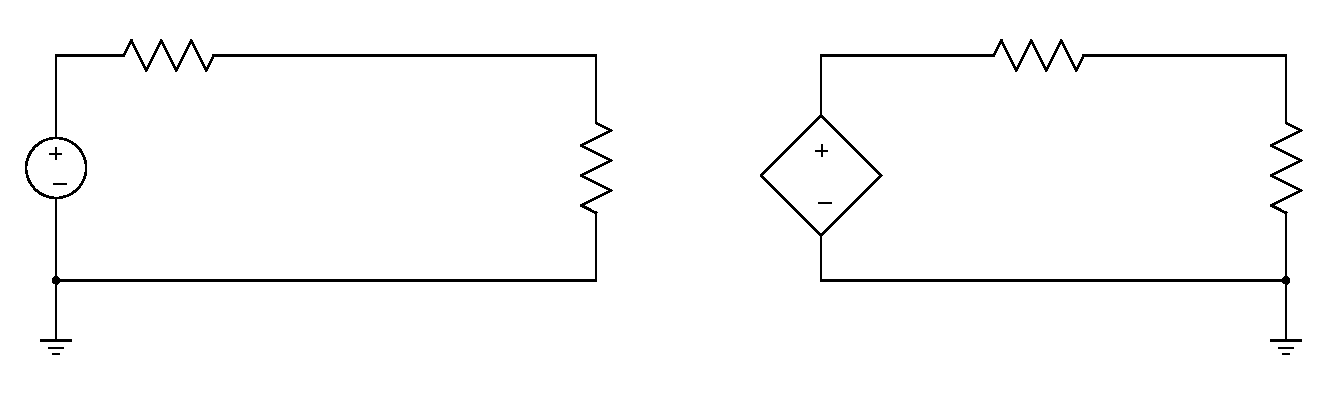
\includegraphics[scale=0.90]{voltageAmplifierTheveninEquivalent}
\caption{برقی دباو ایمپلیفائر کا مساوی تھوِنن  دور}
\label{شکل_واپسی_دباو_ایمپلیفائر_تھیونن_مساوی}
\end{figure}
داخلی جانب برقی رو کو \عددیء{I_i}  لکھتے ہوئے کرخوف کا قانون برائے برقی دباو استعمال کرتے ہیں۔
\begin{align*}
V_s=I_i R_s+I_i R_i \\
I_i = \frac{V_s}{R_s +R_i}
\end{align*}
اور یوں
\begin{align}
V_i=I_i R_i =V_s \left(\frac{R_i}{R_s+R_i} \right)
\end{align}
حاصل ہوتا ہے۔اسی طرح خارجی جانب برقی رو کو \عددیء{I_o} لکھتے ہوئے حاصل  ہوتا ہے
\begin{gather}
\begin{aligned}\label{مساوات_واپسی_بنیادی_خارجی_حقائق_الف}
A_v V_i = I_o R_o + I_o R_L\\
I_o=\frac{A_v V_i}{R_o + R_L}\\
V_o=I_o R_L = A_v V_i  \left(\frac{R_L}{R_o+R_L}\right)
\end{aligned}
\end{gather}
اس مساوات میں \عددیء{V_i} کی قیمت استعمال کرتے حاصل ہوتا ہے
\begin{gather} \label{مساوات_واپسی_دباو_ایمپلیفائر_کی_افزائش}
\begin{aligned}
V_o=A_v V_s \left (\frac{R_L }{R_o+R_L} \right)  \left (\frac{R_i}{R_s+R_i} \right) \\
A_V=\frac{V_o}{V_s}=A_v \left(\frac{R_L}{R_o+R_L} \right) \left(\frac{R_i}{R_s+R_i} \right )
\end{aligned}
\end{gather}
اس مساوات کے تحت افزائش کی قیمت اشارے کے مزاحمت \عددیء{R_s} اور  بوجھ کے مزاحمت \عددیء{R_L} پر منحصر ہے جب کہ ایسا نہیں ہونا چاہیے۔آئیں دیکھیں کہ \عددیء{R_s} اور  \عددیء{R_L} کے اثر کو کیسے ختم یا کم سے کم کیا جا سکتا ہے۔

برقی دباو ایمپلیفائر میں اگر 
\begin{gather} \label{مساوات_قامل_واپسی_دباو_ایمپلیفائر_کے_مزاحمت}
\begin{aligned}
R_i \to \infty \\
R_o \to 0
\end{aligned}
\end{gather}
ہوں تب مساوات \حوالہ{مساوات_واپسی_دباو_ایمپلیفائر_کی_افزائش}  سے
\begin{align} \label{مساوات_واپسی_کامل_دباو_ایمپلیفائر_کی_افزائش}
A_V = A_v
\end{align}
حاصل ہوتا ہے۔ایسا ایمپلیفائر جس کی کل افزائش \عددیء{A_V} کا دارومدار اشارے کی مزاحمت \عددیء{R_s} اور بوجھ کے مزاحمت \عددیء{R_L} پر قطعاً منحصر نہیں ہو اور جس کے \عددیء{A_V}  کی قیمت اٹل ہو کو \اصطلاح {برقی دباو ایمپلیفائر} کہتے ہیں۔شکل \حوالہ{شکل_واپسی_دباو_ایمپلیفائر_تھیونن_مساوی} میں دکھایا، مساوات \حوالہ{مساوات_قامل_واپسی_دباو_ایمپلیفائر_کے_مزاحمت} پر پورا اترتا دور کامل برقی دباو ایمپلیفائر کا دور ہے۔ 

 حقیقی برقی دباو ایمپلیفائر مساوات \حوالہ{مساوات_قامل_واپسی_دباو_ایمپلیفائر_کے_مزاحمت} کی بجائے مساوات \حوالہ{مساوات_حقیقی_واپسی_دباو_ایمپلیفائر_کے_مزاحمت} پر پورا اترتا ہے۔
\begin{gather} \label{مساوات_حقیقی_واپسی_دباو_ایمپلیفائر_کے_مزاحمت}
\begin{aligned}
R_i \gg R_s \\
R_0 \ll R_L
\end{aligned}
\end{gather}
جس کے لئے ہم لکھ سکتے ہیں
\begin{align}  \label{مساوات_واپسی_حقیقی_دباو_ایمپلیفائر_کی_افزائش}
A_V \approx A_v
\end{align}
مساوات \حوالہ{مساوات_واپسی_بنیادی_خارجی_حقائق_الف} سے آپ دیکھ سکتے ہیں کہ لامحدود \عددیء{R_L} پر \عددیء{\frac{V_o}{V_i}} کی قیمت \عددیء{A_v} کے برابر ہے یعنی
\begin{align}
A_v = \left . \frac{V_o}{V_i} \right |_{R_L \to \infty}
\end{align} 
لہٰذا \عددیء{A_v} کو ایمپلیفائر کی لامحدود بوجھ کے مزاحمت پر افزائش برقی دباو پکارا جاتا ہے۔اسے بے بوجھ ایمپلیفائر کی افزائش برقی دباو  بھی پکارا جا سکتا ہے۔

 
شکل \حوالہ{شکل_واپسی_دباو_ایمپلیفائر_ڈبہ_شکل} الف میں برقی دباو ایمپلیفائر میں داخلی اشارے کی مزاحمت \عددیء{R_s} کو بھی ایمپلیفائر کا حصہ تصور کرتے ہوئے شکل  ب میں اسی کا سادہ ڈبہ نما شکل دکھایا گیا ہے۔
\begin{figure}
\centering
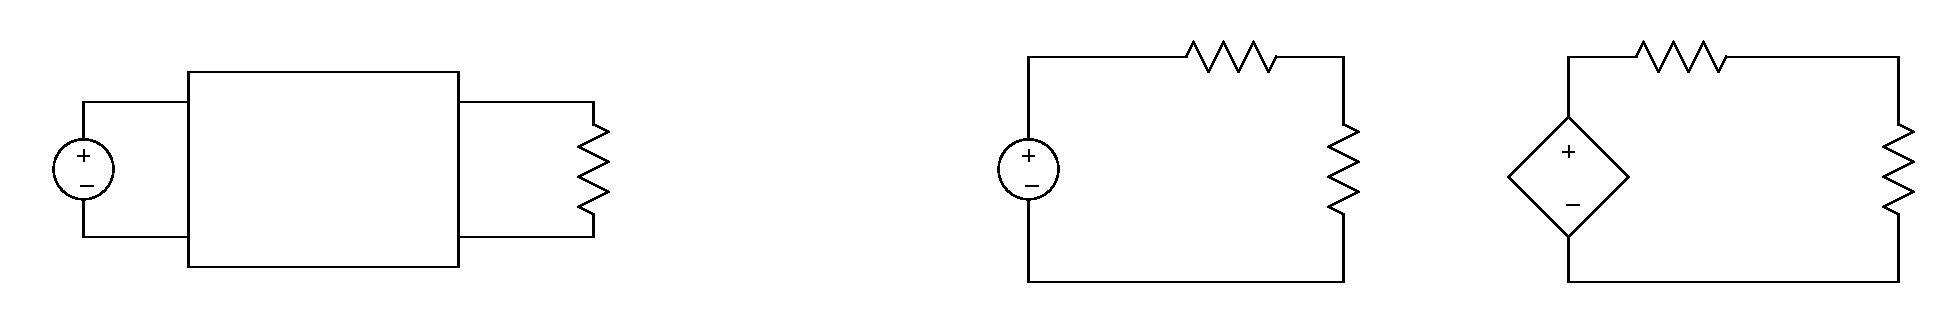
\includegraphics[scale=0.90]{voltageAmplifierTheveninEquivalentA}
\caption{برقی دباو ایمپلیفائر کا سادہ ڈبہ نما شکل}
\label{شکل_واپسی_دباو_ایمپلیفائر_ڈبہ_شکل}
\end{figure}


\جزوحصہ{برقی رو ایمپلیفائر}
برقی رو ایمپلیفائر کا مساوی نارٹن  دور شکل \حوالہ{شکل_واپسی_رو_ایمپلیفائر_نارٹن_مساوی} میں نقطہ دار لکیر میں بند دکھایا گیا ہے۔ اسے داخلی جانب اشارہ \عددیء{I_s} مہیا کیا گیا ہے جبکہ خارجی جانب اس پر برقی بوجھ \عددیء{R_L} لادا گیا ہے۔ منبع داخلی اشارے کی مزاحمت \عددیء{R_s} ہے۔
\begin{figure}
\centering
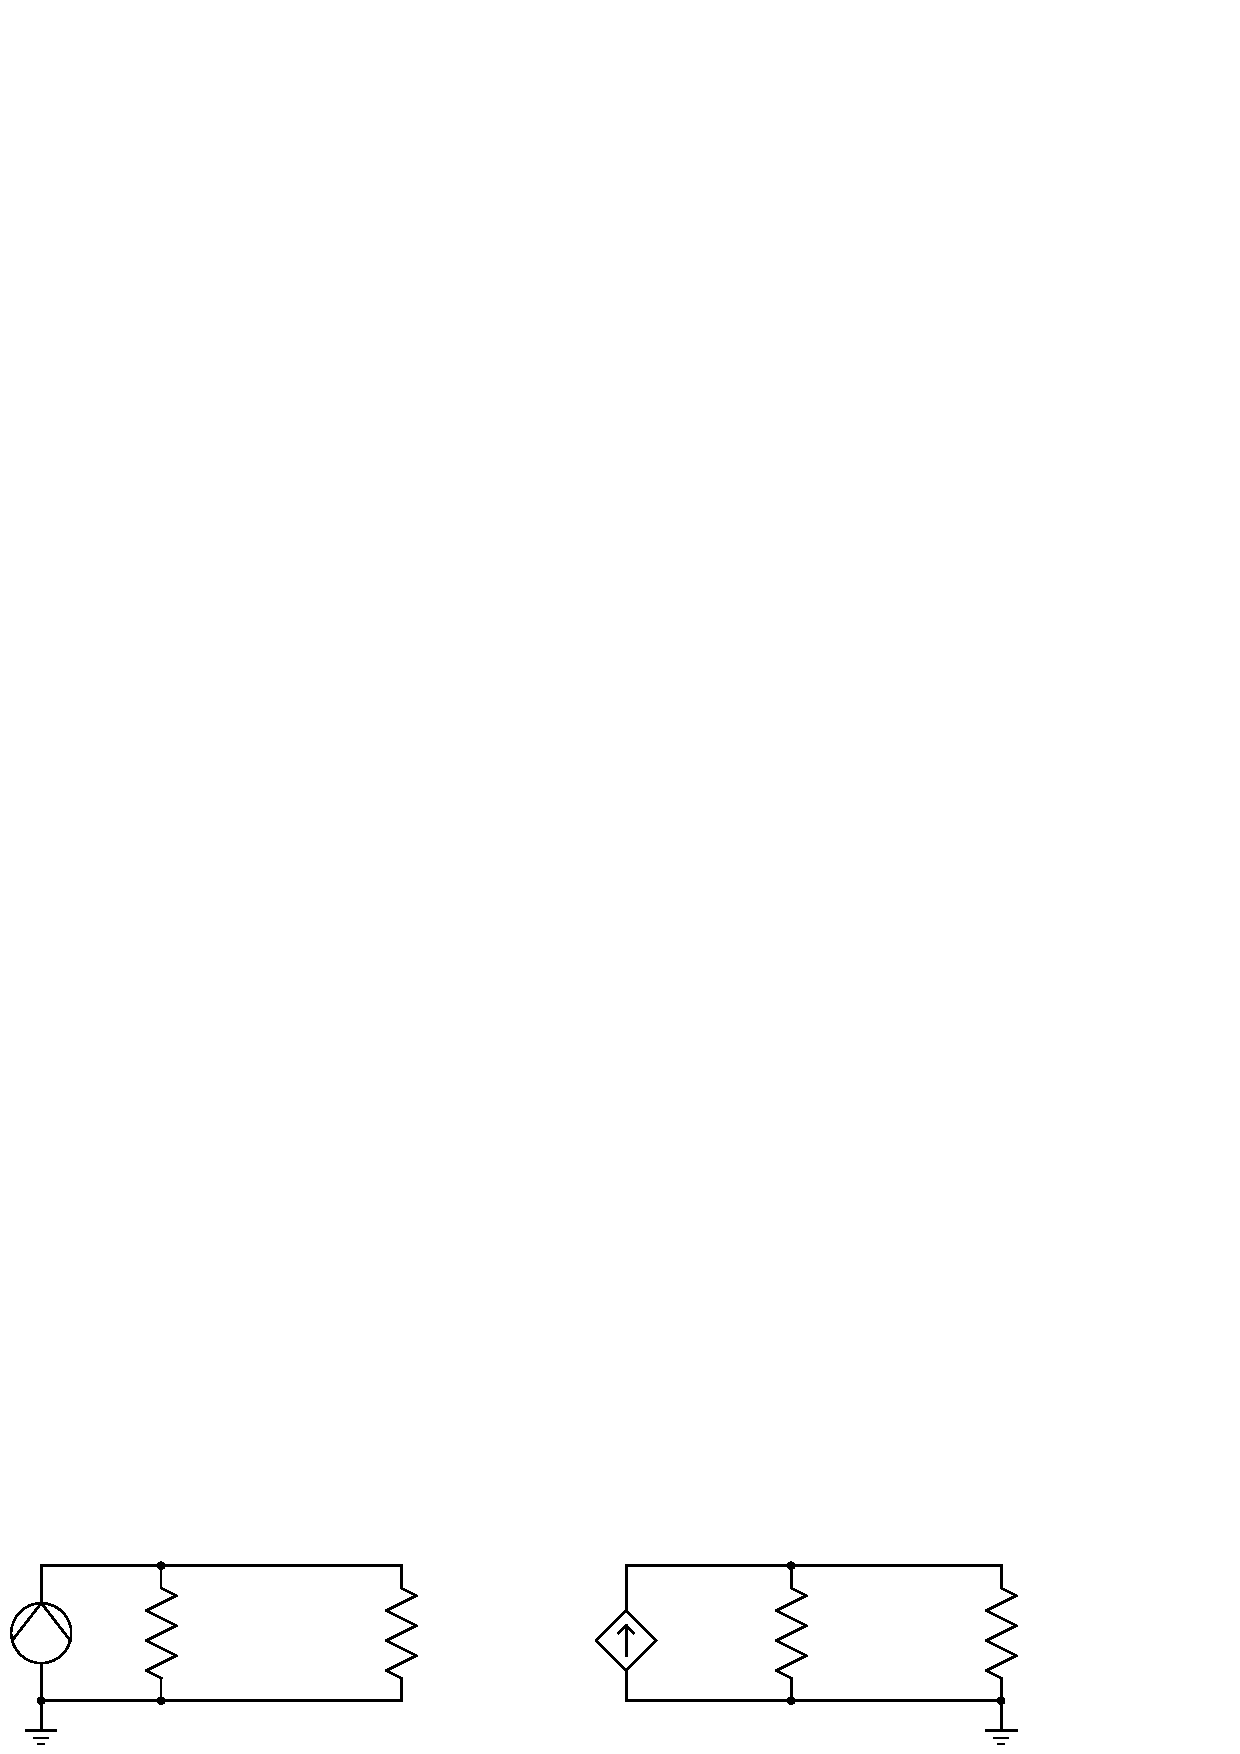
\includegraphics[scale=0.90]{currentAmplifierNortonEquivalent}
\caption{برقی رو ایمپلیفائر کا مساوی نارٹن دور}
\label{شکل_واپسی_رو_ایمپلیفائر_نارٹن_مساوی}
\end{figure}
داخلی جانب تقسیم برقی رو سے حاصل ہوتا ہے
\begin{align}
I_i = I_s  \left (\frac{R_s}{R_s+R_i} \right )
\end{align}
اسی طرح خارجی جانب تقسیم برقی رو سے حاصل ہوتا ہے
\begin{align} \label{مساوات_واپسی_رو_ایمپلیفائر_کی_خارجی_رو}
I_o = A_i I_i \left (\frac{R_o}{R_o+R_L} \right )
\end{align}
مندرجہ بالا دو مساوات سے حاصل ہوتا ہے
\begin{align}
I_o = A_i  I_s \left (\frac{R_s}{R_s+R_i} \right )  \left(\frac{R_o}{R_o+R_L} \right)
\end{align}
جس سے کل افزائش برقی رو \عددیء{A_I} یوں حاصل ہوتی ہے
\begin{align} \label{مساوات_واپسی_رو_ایمپلیفائر_کی_افزائش}
A_I = \frac{I_o}{I_s}=A_i \left(\frac{R_s}{R_s+R_i} \right)  \left (\frac{R_o}{R_o+R_L} \right)
\end{align}
مساوات \حوالہ{مساوات_واپسی_رو_ایمپلیفائر_کی_افزائش} میں اگر 
\begin{gather} \label{مساوات_واپسی_رو_ایمپلیفائر_کے_مزاحمت_کی_شرط}
\begin{aligned}
R_i \ll R_s \\
R_o \gg R_L
\end{aligned}
\end{gather}
ہوں تو اسے یوں لکھا جا سکتا ہے
\begin{align} \label{مساوات_واپسی_کامل_رو_ایمپلیفائر_کی_افزائش}
A_I  \approx A_i 
\end{align}

ایسا ایمپلیفائر جس کی افزائش \عددیء{A_I} کا دارومدار داخلی بیرونی مزاحمت \عددیء{R_s} اور خارجی بیرونی مزاحمت \عددیء{R_L} پر قطعاً منحصر نہیں ہو اور جس کے \عددیء{A_I} کی قیمت اٹل ہو کو \اصطلاح {برقی رو ایمپلیفائر} کہتے ہیں۔برقی رو ایمپلیفائر مساوات \حوالہ{مساوات_واپسی_رو_ایمپلیفائر_کے_مزاحمت_کی_شرط} کے تحت ہی تخلیق دئے جاتے ہیں تا کہ ان کی افزائش زیادہ سے زیادہ ہو اور اس کی قیمت خارجی مزاحمت  پر منحصر نہ ہو۔ کامل برقی رو ایمپلیفائر میں \عددیء{R_i=0} اور \عددیء{R_o=\infty} ہوں گے۔مساوات \حوالہ{مساوات_واپسی_رو_ایمپلیفائر_کی_خارجی_رو} سے آپ دیکھ سکتے ہیں کہ \عددیء{R_L=0} کی صورت میں 
\begin{align} \label{مساوات_واپسی_صفر_بار_مزاحمت_پر_رو_کی_افزائش}
\left . \frac{I_o}{I_i} \right|_{R_L=0}=A_i
\end{align}
حاصل ہوتا ہے، لہٰذا \عددیء{A_i} کو صفر بوجھ کے مزاحمت پر ایمپلیفائر کی افزائش برقی رو پکارا جائے گا۔


\جزوحصہ{موصل نما ایمپلیفائر}
آپ نے برقی دباو اور برقی رو ایمپلیفائر کے مساوی دور دیکھے۔دباو ایمپلیفائر کا تھوِنن  مساوی جبکہ رو ایمپلیفائر کا نارٹن مساوی دور استعمال کیا گیا۔یہاں اس بات کا سمجھنا ضروری ہے کہ جہاں برقی دباو کی بات کی جائے وہاں تھوِنن  مساوی دور استعمال کیا جاتا ہے اور جہاں برقی رو کی بات کی جائے وہاں نارٹن مساوی دور استعمال کیا جاتا ہے۔یوں چونکہ برقی دباو ایمپلیفائر داخلی برقی دباو کو بڑھاتا ہے لہٰذا داخلی جانب اشارہ منبع کا تھوِنن  مساوی دور استعمال کیا گیا۔اسی طرح چونکہ یہ ایمپلیفائر برقی دباو ہی خارج کرتا ہے لہٰذا خارجی جانب ایمپلیفائر کا تھوِنن  مساوی دور ہی استعمال کیا گیا۔

برقی رو ایمپلیفائر کا داخلی اشارہ برقی رو ہوتا ہے لہٰذا داخلی جانب اشارہ منبع کا نارٹن مساوی دور استعمال کیا جاتا ہے۔اسی طرح یہ ایمپلیفائر برقی رو ہی خارج کرتا ہے لہٰذا خارجی جانب بھی نارٹن مساوی دور استعمال کیا گیا۔

موصل نما ایمپلیفائر کا داخلی اشارہ برقی دباو جبکہ اس کا خارجی اشارہ برقی رو ہوتا ہے لہٰذا اس کا تجزیہ کرتے وقت داخلی جانب اشارہ منبع کا تھوِنن  جبکہ اس کے خارجی جانب نارٹن مساوی دور استعمال کیا جائے گا۔شکل \حوالہ{شکل_واپسی_موصلیت_نما_ایمپلیفائر_کا_مساوی_دور} میں موصل نما ایمپلیفائر کا مساوی دور دکھایا گیا ہے۔
\begin{figure}
\centering
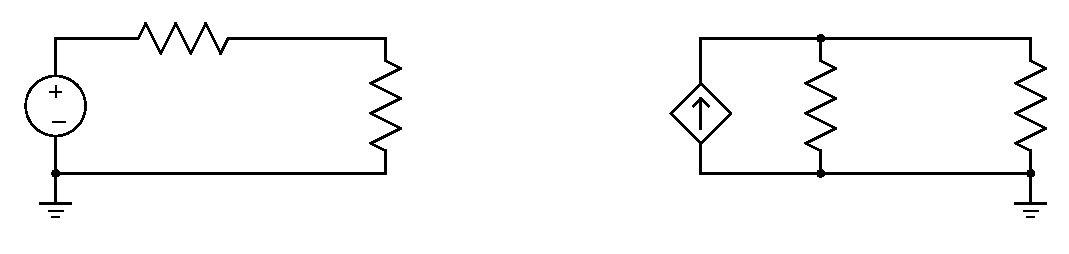
\includegraphics[scale=0.90]{transconductanceAmplifierEquivalent}
\caption{موصل نما ایمپلیفائر کا مساوی دور}
\label{شکل_واپسی_موصلیت_نما_ایمپلیفائر_کا_مساوی_دور}
\end{figure}
موصل نما ایمپلیفائر کے لئے ہم لکھ سکتے ہیں
\begin{gather} \label{مساوات_واپسی_موصلیت_نما_خارجی_رو}
\begin{aligned}
V_i = V_s \left(\frac{R_i}{R_i+R_s}\right)\\
I_o=A_g V_i \left(\frac{R_o}{R_o+R_L}\right) \\
I_o = A_g V_s  \left (\frac{R_i}{R_i+R_s} \right ) \left(\frac{R_o}{R_o+R_L} \right )
\end{aligned}
\end{gather}
لہٰذا
\begin{align} \label{مساوات_واپسی_کل_موصلیت_نما}
A_G=\frac{I_o}{V_s}=A_g \left (\frac{R_i}{R_i+R_s} \right ) \left(\frac{R_o}{R_o+R_L} \right )
\end{align}

مساوات \حوالہ{مساوات_واپسی_موصلیت_نما_خارجی_رو} سے آپ دیکھ سکتے ہیں کہ \عددیء{R_L=0} کی صورت میں \عددیء{\frac {ِI_o}{V_i}} کی قیمت \عددیء{A_g} کے برابر ہے یعنی 
\begin{align}
\left.  \frac{I_o}{V_i} \right |_{R_L =0} =A_g
\end{align}
اسی طرح 
\begin{gather}
\begin{aligned}
R_i \gg R_s \\
R_o \gg R_L
\end{aligned}
\end{gather}
 کی صورت میں مساوات  \حوالہ{مساوات_واپسی_کل_موصلیت_نما} سے حاصل ہوتا ہے
\begin{align}
A_G \approx A_g
\end{align}
ایسا ایمپلیفائر جس کی افزائش \عددیء{A_G} کا دارومدار \عددیء{R_s} اور مزاحمت \عددیء{R_L} پر قطعاً منحصر نہیں ہو اور جس کے \عددیء{A_G} کی قیمت اٹل ہو کو \اصطلاح {موصل نما ایمپلیفائر} کہتے ہیں۔

\جزوحصہ{مزاحمت نما ایمپلیفائر}
شکل \حوالہ{شکل_واپسی_مزاحمت_نما_ایمپلیفائر_کا_مساوی_دور} میں مزاحمت نما ایمپلیفائر دکھایا گیا ہے جس کا داخلی اشارہ برقی رو \عددیء{I_s} اور خارجی اشارہ برقی دباو \عددیء{V_o} ہے۔ اس کو یوں حل کیا جائے گا۔
\begin{figure}
\centering
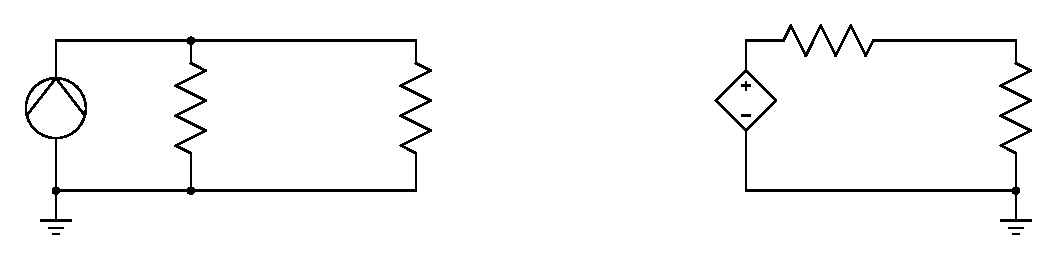
\includegraphics[scale=0.90]{transresistanceAmplifierEquivalent}
\caption{مزاحمت نما ایمپلیفائر کا مساوی دور}
\label{شکل_واپسی_مزاحمت_نما_ایمپلیفائر_کا_مساوی_دور}
\end{figure}
%
\begin{gather} \label{مساوات_واپسی_مزاحمت_نما_ایمپلیفائر_کے_مساوات}
\begin{aligned}
I_i=I_s \left(\frac{R_s}{R_s+R_i}\right) \\
V_o=A_r I_i \left(\frac{R_L}{R_L+R_o}\right)
\end{aligned}
\end{gather}
اس مساوات سے ہم دیکھتے ہیں کہ \عددیء{R_L = \infty} کی صورت میں \عددیء{\frac{V_o}{I_i}} کی قیمت \عددیء{A_r} کے برابر ہو گی یعنی
\begin{align}
\left . \frac{V_o}{I_i} \right |_{R_L = \infty}=A_r
\end{align}
لہٰذا \عددیء{A_r} کو لامحدود مزاحمتی بوجھ پر ایمپلیفائر کی \اصطلاح {مزاحمت نما افزائش}  کہتے ہیں۔کل مزاحمت نما افزائش \عددیء{A_R} مساوات \حوالہ{مساوات_واپسی_مزاحمت_نما_ایمپلیفائر_کے_مساوات} سے حاصل کرتے ہیں۔
\begin{align} \label{مساوات_واپسی_کل_مزاحمت_نما}
A_R=\frac{V_o}{I_s}=A_r \left( \frac{R_s}{R_s+R_i} \right ) \left ( \frac{R_L}{R_L +R_o} \right )
\end{align}
آپ دیکھ سکتے ہیں کہ 
\begin{gather}
\begin{aligned} \label{مساوات_واپسی_حقیقی_مزاحمت_نما_ایمپلیفائر_کے_مزاحمت}
R_i \ll R_s \\
R_o \ll R_L
\end{aligned}
\end{gather}
 کی صورت میں مساوات \حوالہ{مساوات_واپسی_کل_مزاحمت_نما} کو یوں لکھا جا سکتا ہے
\begin{align} \label{مساوات_واپسی_کل_مزاحمت_نما_تقریبا_اٹل_ہے}
A_R \approx A_r
\end{align}
یعنی اس صورت ایمپلیفائر کی مزاحمت نما افزائش کا دارومدار \عددیء{R_s} اور \عددیء{R_L} پر نہیں۔

 
%---------
\ابتدا{مثال}
شکل \حوالہ{شکل_واپسی_دباو_ایمپلیفائر_تھیونن_مساوی} میں بوجھ کے مزاحمت \عددیء{R_L} میں برقی رو کی قیمت \عددیء{\frac{V_o}{R_L}}  کے برابر  ہے۔ \عددیء{\frac{I_o}{V_s}}  کی شرح کو موصل نما افزائش تصور کرتے ہوئے ثابت کریں کہ اسے موصل نما ایمپلیفائر تصور نہیں کیا جا سکتا۔

حل:
\begin{equation*}
A_G=\frac{I_o}{V_s}=\frac{I_o}{V_o} \times \frac{V_o}{V_s}=\frac{1}{R_L} \times A_V
\end{equation*}
اس مساوات کے تحت \عددیء{A_G} کی قیمت بوجھ کے مزاحمت \عددیء{R_L} کے قیمت پر منحصر ہے۔ایمپلیفائر کی افزائش کی قیمت بوجھ کے مزاحمت کے قیمت پر منحصر نہیں ہو سکتی لہٰذا اسے موصل نما ایمپلیفائر تصور نہیں کیا جا سکتا۔ 

\انتہا{مثال}

\حصہ{واپسی اشارہ}
مندرجہ بالا حصے میں ہم نے چار اقسام کے ایمپلیفائر دیکھے۔ اس حصے میں ان میں واپسی اشارہ شامل کرنے کی ترکیب دکھائی جائے گی۔واپسی اشارے کو ایمپلیفائر کے داخلی اشارے کے ساتھ جمع یا اس سے منفی کیا جاتا ہے۔

 شکل \حوالہ{شکل_واپسی_اشارات_جمع_منفی_کے_طریقے} الف  میں واپسی اشارے \عددیء{V_f} کو برقی دباو اشارے \عددیء{V_s} کے ساتھ  جمع کرنا دکھایا گیا ہے جبکہ شکل \حوالہ{شکل_واپسی_اشارات_جمع_منفی_کے_طریقے} ب میں  \عددیء{V_f} کو \عددیء{V_s} سے منفی کرنا دکھایا گیا ہے۔ شکل  پ  میں واپسی اشارے \عددیء{I_f} کو برقی رو اشارے  \عددیء{I_s} کے ساتھ جمع کرنا دکھایا گیا ہے جبکہ شکل  ت میں \عددیء{I_f} کو  \عددیء{I_s} سے منفی کرنا دکھایا گیا ہے۔برقی دباو اشارات کو آپس میں جمع یا منفی کرتے وقت انہیں سلسلہ وار جوڑا جاتا ہے جبکہ برقی رو اشارات کو آپس میں جمع یا منفی کرتے وقت انہیں متوازی جوڑا جاتا ہے۔برقی دباو اشارے کو کسی صورت برقی رو اشارے کے ساتھ جمع یا منفی نہیں کیا جا سکتا۔ \حاشیہد{آپ جانتے ہیں کہ آلو اور ٹماٹر کو آپس میں جمع یا منفی نہیں کیا جا سکتا۔اسی طرح برقی دباو کو صرف اور صرف برقی دباو کے ساتھ ہی جمع یا اس سے منفی کیا جا سکتا ہے۔}

شکل \حوالہ{شکل_واپسی_دباو_ایمپلیفائر_ڈبہ_شکل} ب میں دکھائے برقی دباو ایمپلیفائر کو مثال بناتے ہیں۔برقی دباو ایمپلیفائر داخلی جانب اشارات کو برقی دباو کی صورت میں حاصل کرتا ہے لہٰذا اس کے داخلی جانب واپسی اشارہ بھی برقی دباو کی صورت میں ہو گا۔
\begin{figure}
\centering
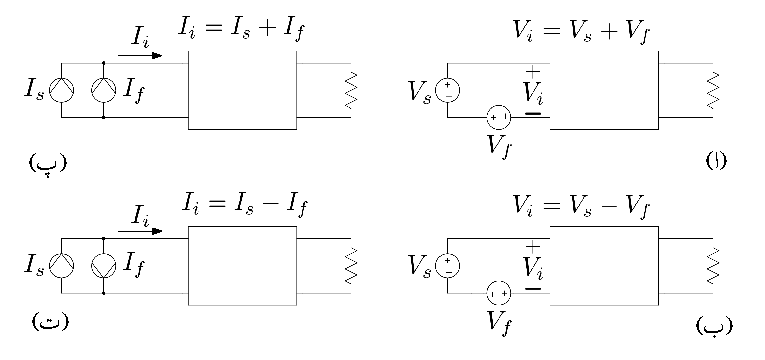
\includegraphics[scale=0.90]{positiveNegativeFeedback}
\caption{اشارات کو آپس میں جمع اور منفی کرنے کے طریقے}
\label{شکل_واپسی_اشارات_جمع_منفی_کے_طریقے}
\end{figure}
واپسی اشارے کو ایمپلیفائر کے خارجی اشارے سے حاصل کیا جاتا ہے۔ \عددیء{V_o} سے \عددیء{V_f} حاصل کرنے والے دور، جس کو \اصطلاح {واپس کار}\فرہنگ{واپس کار}\حاشیہب{feedback circuit} کہتے ہیں، کو ڈبے کی شکل سے دکھاتے ہوئے شکل \حوالہ{شکل_واپسی_ایمپلیفائر_کے_اقسام} الف حاصل ہوتا ہے جسے \اصطلاح {واپسی برقی دباو ایمپلیفائر}\فرہنگ{واپسی!برقی دباو ایمپلیفائر}\فرہنگ{ایمپلیفائر!واپسی} کہا جائے گا۔اس شکل میں اوپر والا ڈبہ بنیادی برقی دباو ایمپلیفائر ہے جبکہ نچلا ڈبہ واپس کار ہے۔واپس کار کا داخلی اشارہ \عددیء{V_o} ہے جبکہ اس کا خارجی واپسی اشارہ \عددیء{V_f} ہے۔واپس کار  کا داخلی  اشارہ بنیادی ایمپلیفائر کے خارجی جانب سے   متوازی حاصل کیا جاتا ہے جبکہ \عددیء{V_f} کو \عددیء{V_s}  کے ساتھ  سلسلہ وار جوڑا گیا ہے۔

اس شکل میں واپسی اشارے \عددیء{V_f} کو اشارہ \عددیء{V_s} سے منفی کیا گیا ہے اور یوں اس ایمپلیفائر کو \اصطلاح {منفی واپسی برقی دباو ایمپلیفائر}\فرہنگ{منفی واپسی برقی دباو ایمپلیفائر}\حاشیہب{negative feedback voltage amplifier} کہا جائے گا۔اگر  \عددیء{V_f} کو \عددیء{V_s} کے ساتھ جمع کیا جاتا تب اسے  \اصطلاح {جمع واپسی برقی دباو ایمپلیفائر}\فرہنگ{ایمپلیفائر!واپسی}\حاشیہب{positive feedback voltage amplifier} کہا جاتا۔اس باب میں \اصطلاح {منفی واپسی ایمپلیفائر} پر ہی بحث کی جائے گی۔اگلے باب میں \اصطلاح {جمع واپسی ادوار} کا استعمال کیا جائے گا۔
\begin{figure}
\centering
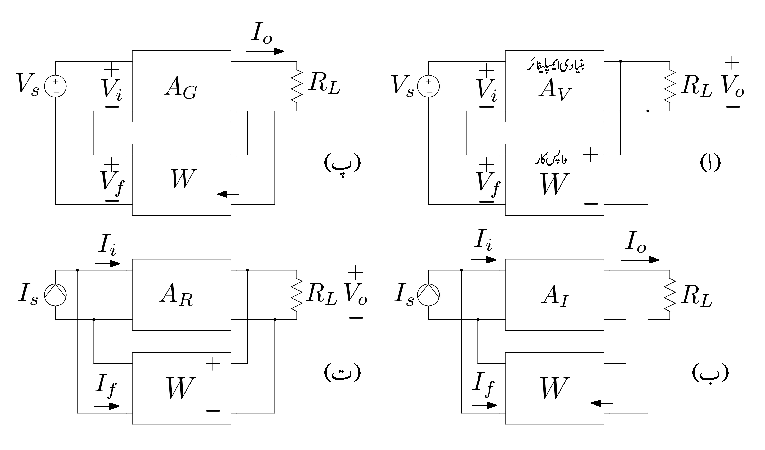
\includegraphics[scale=0.90]{feedbackTopologies}
\caption{واپسی ایمپلیفائر کے اقسام}
\label{شکل_واپسی_ایمپلیفائر_کے_اقسام}
\end{figure}

شکل \حوالہ{شکل_واپسی_ایمپلیفائر_کے_اقسام} ب میں برقی رو ایمپلیفائر میں واپسی اشارے کی شمولیت دکھائی گئی ہے۔بنیادی ایمپلیفائر کے داخلی جانب \عددیء{I_s} سے \عددیء{I_f} منفی کیا گیا ہے۔یوں اس مکمل دور کو \اصطلاح {منفی واپسی برقی رو ایمپلیفائر}\فرہنگ{منفی واپسی برقی رو ایمپلیفائر}\حاشیہب{negative feedback current amplifier} کہا جائے گا۔واپسی اشارے کو خارجی اشارہ \عددیء{I_o} سے حاصل کیا گیا ہے۔ایسا کرنے کی خاطر واپس کار کے  داخلی جانب کو بنیادی ایمپلیفائر کے خارجی جانب کے ساتھ سلسلہ وار جوڑا گیا ہے تا کہ خارجی برقی رو \عددیء{I_o} واپس کار کو بطور داخلی اشارہ مہیا کیا جا سکے۔

یہاں رک کر اس بات کو سمجھیں کہ خارجی برقی دباو \عددیء{V_o} سے واپسی اشارہ حاصل کرتے وقت واپس کار کے داخلی جانب کو بنیادی ایمپلیفائر کے خارجی جانب  متوازی جوڑا جاتا ہے جبکہ خارجی برقی رو \عددیء{I_o} سے واپسی اشارہ حاصل کرتے وقت واپس کار کا داخلی جانب اور بنیادی ایمپلیفائر کا خارجی جانب سلسلہ وار جوڑے جاتے ہیں۔واپسی اشارہ ازخود برقی دباو یا برقی رو کی صورت میں ہو سکتا ہے۔

شکل \حوالہ{شکل_واپسی_ایمپلیفائر_کے_اقسام} پ میں  موصل نما ایمپلیفائر میں واپسی اشارہ شامل کرنا دکھایا گیا ہے۔یہاں بنیادی ایمپلیفائر کا خارجی اشارہ برقی رو \عددیء{I_o} ہے جس سے واپسی اشارہ حاصل کیا جاتا ہے لہٰذا واپس کار کے داخلی جانب کو بنیادی ایمپلیفائر کے خارجی جانب  سلسلہ وار جوڑا گیا ہے۔واپس کار کا خارجی اشارہ برقی دباو \عددیء{V_f} ہے جسے \عددیء{V_s} سے منفی کیا گیا ہے۔

شکل \حوالہ{شکل_واپسی_ایمپلیفائر_کے_اقسام} ت میں مزاحمت نما ایمپلیفائر میں واپسی اشارے کی شمولیت دکھائی گئی ہے جسے آپ خود سمجھ سکتے ہیں۔

جہاں متن سے واضح ہو وہاں ان ایمپلیفائر کے پورے نام کی جگہ صرف واپسی ایمپلیفائر کا نام استعمال کیا جائے گا۔


%+++++++++

\حصہ{بنیادی کارکردگی}
ٹرانزسٹر ایمپلیفائر کے دور میں ٹرانزسٹر کا ریاضی نمونہنسب کرتے ہوئے انہیں کرخوف کے قوانین سے حل کرنے سے آپ بخوبی واقف ہیں۔واپسی ایمپلیفائر کو بھی اسی طرح حل کرنا ممکن ہے البتہ انہیں یوں حل کرنے سے واپسی عمل کی وضاحت نہیں ہوتی۔اس حصے میں ہم واپسی ایمپلیفائر کو اس طرح حل کریں گے کہ ان میں واپسی اشارے کا کردار اجاگر ہو۔

واپسی ادوار کے تین جزو ہیں۔پہلا جزو بنیادی ایمپلیفائر، دوسرا جزو جمع کار (یا منفی کار) اور تیسرا جزو واپس کار۔شکل \حوالہ{شکل_بنیادی_واپسی_ایمپلیفائر} میں ان تینوں اجزاء کو دکھایا گیا ہے۔

یہاں بنیادی ایمپلیفائر سے مراد حصہ \حوالہ{حصہ_واپسی_ایمپلیفائر_کی_جماعت_بندی} میں دکھائے چار قسم کے ایمپلیفائر میں سے کوئی بھی ہو سکتا ہے۔اشارے کی مزاحمت \عددیء{R_s} کو یہاں بنیادی ایمپلیفائر کا حصہ تصور کیا گیا ہے۔ یوں شکل \حوالہ{شکل_بنیادی_واپسی_ایمپلیفائر} میں \عددیء{A} سے مراد \عددیء{A_V} ، \عددیء{A_I} ، \عددیء{A_G} یا \عددیء{A_R} ہو سکتا ہے۔ یہاں \عددیء{R_L} کے علاوہ واپس کار کا داخلی جانب  بھی ایمپلیفائر کے خارجی جانب نسب ہے  اور \عددیء{A} واپس کار کے بوجھ کو بھی شامل کرتے حاصل کیا جاتا ہے۔اس کی وضاحت حصہ \حوالہ{حصہ_واپسی_تفصیلی_تجزیہ} میں کی جائے گی۔
\begin{figure}
\centering
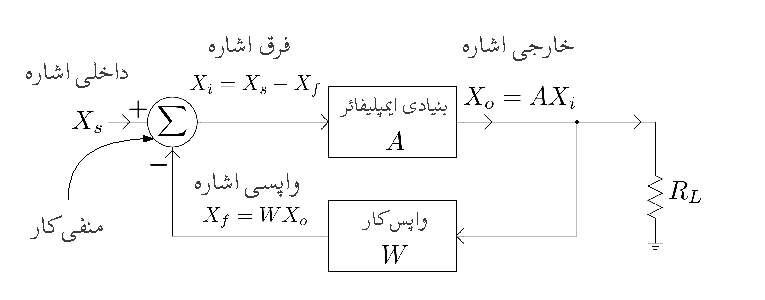
\includegraphics[scale=0.90]{basicFeedback}
\caption{بنیادی واپسی ایمپلیفائر}
\label{شکل_بنیادی_واپسی_ایمپلیفائر}
\end{figure}
ایمپلیفائر کے داخلی اشارے \عددیء{V_s} یا \عددیء{I_s} کو \عددیء{X_s} جبکہ اس کے خارجی اشارے \عددیء{V_o} یا \عددیء{I_o} کو \عددیء{X_o}  اور اسی طرح واپسی اشارے \عددیء{V_f} یا \عددیء{I_f} کو \عددیء{X_f} لکھتے ہوئے آگے بڑھتے ہیں۔یوں اس شکل میں بنیادی ایمپلیفائر اشارہ \عددیء{X_i} کو بڑھا کر بطور \عددیء{X_o} خارج کرتا ہے یعنی
\begin{align}
X_o = A X_i
\end{align}
 اس مساوات کو یوں بھی لکھا جا سکتا ہے
\begin{gather} \label{مساوات_واپسی_افزائش}
\begin{aligned}
A =\frac{X_o}{X_i}
\end{aligned}
\end{gather}
واپس کار عموماً غیر عامل پرزہ جات یعنی مزاحمت، کپیسٹر وغیرہ سے تخلیق دیا جاتا ہے۔یہ  خارجی اشارے کا کچھ حصہ داخلی جانب تک پہنچاتا ہے۔شکل سے آپ دیکھ سکتے ہیں کہ واپس کار  \عددیء{X_o} کا کچھ حصہ منفی کار کو بطور واپسی اشارہ \عددیء{X_f}  پیش کرتا ہے جہاں
\begin{align} \label{مساوات_واپسی_واپسی_اشارہ}
X_f = W X_o
\end{align}
ہے۔\عددیء{W} سے مراد واپس کار کے خارجی اور داخلی اشاروں کی شرح یعنی \عددیء{\frac{X_f}{X_o}} ہے۔\عددیء{W} کو واپس کار کا مستقل\فرہنگ{واپس کار کا مستقل}\حاشیہب{feedback constant} کہا جائے گا۔

منفی کار داخلی اشارے \عددیء{X_s} سے واپسی اشارہ \عددیء{X_f} کو منفی کر کے اسے بطور فرق اشارہ \عددیء{X_i} خارج کرتا ہے یعنی
\begin{align} \label{مساوات_واپسی_فرق_اشارہ}
X_i= X_s - X_f
\end{align}
اس میں مساوات \حوالہ{مساوات_واپسی_واپسی_اشارہ} استعمال کرتے
\begin{align} \label{مساوات_واپسی_ایمپلیفائر_کے_جماعت_بندی}
X_i= X_s - W X_o
\end{align}
ملتا ہے جس میں مساوات \حوالہ{مساوات_واپسی_افزائش} کے استعمال سے
\begin{align*}
\frac{X_o}{A} =X_s - W X_o
\end{align*}
حاصل ہوتا ہے۔ اس کو \عددیء{X_o} کے لئے حل کرتے ہیں
\begin{align*}
X_o =A \left( X_s-W X_o \right) \\
X_o \left (1+ W A \right ) =A X_s \\
X_o =\left(\frac{A}{1+ W A}\right) X_s
\end{align*}
یوں پورے دور کے داخلی اشارے  کو \عددیء{X_s} اور اس کا خارجی اشارے کو \عددیء{X_o} لیتے ہوئے واپسی دور کے کل افزائش \عددیء{A_f} کو یوں لکھ سکتے ہیں۔
\begin{align} \label{مساوات_واپسی_کل_افزائش}
A_f =\frac{X_o}{X_s}=\frac{A}{1+ W A}
\end{align}
منفی واپسی ایمپلیفائر میں \عددیء{\abs{A} > \abs{A_f}}  ہوتا ہے جبکہ مثبت واپسی ایمپلیفائر میں  \عددیء{\abs{A} < \abs{A_f}} ہوتا ہے۔

%--------------
\ابتدا{مثال}
ایک ایمپلیفائر جس کا  \عددیء{A=99} ہے  میں واپسی اشارے کی شمولیت سے واپسی ایمپلیفائر تخلیق دیا جاتا ہے۔\عددیء{W=0.01} اور \عددیء{W=0.1} پر  واپسی ایمپلیفائر کی افزائش \عددیء{A_f} حاصل کریں۔ 

حل:

مساوات \حوالہ{مساوات_واپسی_کل_افزائش} کی مدد سے  \عددیء{W=0.01} پر
\begin{align*}
A_f = \frac{99}{1+0.01 \times 99}=\num{49.749}
\end{align*} 
جبکہ  \عددیء{W=0.1} پر
\begin{align*}
A_f = \frac{99}{1+0.1 \times 99}=\num{9.0826}
\end{align*} 
 حاصل ہوتا ہے۔منفی واپسی ایمپلیفائر کی افزائش واضح طور کم ہوئی ہے۔ 

\انتہا{مثال}
%--------------
\جزوحصہ{افزائشی دائرہ}
واپسی ایمپلیفائر میں بنیادی ایمپلیفائر اور واپسی دور بند دائرے کی شکل میں آپس میں جوڑے جاتے ہیں۔شکل \حوالہ{شکل_بنیادی_واپسی_ایمپلیفائر_شرح_دائرہ} الف میں اس دائرے کو واپسی دور کے خارجی نقطے   پر کھلے سرے کر دیا گیا ہے جبکہ داخلی اشارے کو منقطع کر دیا گیا ہے۔فرض کریں کہ اس نقطے  کے بائیں جانب اشارہ \عددیء{X} پایا جاتا ہے۔اس نقطے  سے دائرے میں گھڑی کے سمت چلتے ہوئے ہم دیکھتے ہیں کہ اشارہ \عددیء{X} پہلے \عددیء{-1} سے ضرب ہو کر \عددیء{-X} ہوتا ہے۔اس کے بعد ایمپلیفائر سے گزرتے ہوئے \عددیء{A} سے ضرب ہو کر \عددیء{-AX} ہو جاتا ہے اور آخر کار واپسی دور سے گزرتے ہوئے \عددیء{W} سے ضرب کھا کر \عددیء{-WAX} ہو جاتا ہے۔یوں یہ اشارہ پورے دائرے سے گزرتے ہوئے \عددیء{-WA} سے ضرب ہوتا ہے جسے واپسی ایمپلیفائر کا \اصطلاح {افزائشی دائرہ}\فرہنگ{افزائشی دائرہ}\فرہنگ{loop gain}\حاشیہب{loop gain} کہا جائے گا۔ شکل  ب میں دائرے کو ایک اور جگہ سے کھلے سرے کرتے ہوئے یہی عمل دکھایا گیا ہے۔آپ دیکھ سکتے ہیں کہ دائرے کو کہیں سے بھی کھلے سرے کرتے ہوئے اس نقطے  سے گھڑی کی سمت پورا چکر کاٹتے ہوئے اشارہ \عددیء{-WA} سے ہی ضرب ہوتا ہے۔
\begin{figure}
\centering
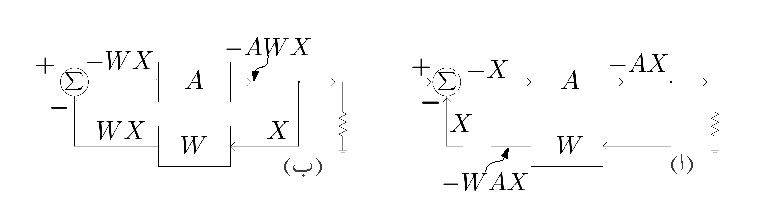
\includegraphics[scale=0.90]{basicFeedbackA}
\caption{بنیادی واپسی ایمپلیفائر کا شرح دائرہ}
\label{شکل_بنیادی_واپسی_ایمپلیفائر_شرح_دائرہ}
\end{figure}

\جزوحصہ{بنیادی مفروضے}\شناخت{حصہ_واپسی_مفروضے}
واپسی ایمپلیفائر پر بات کرتے ہوئے مندرجہ ذیل مفروضے  تصور کئے جائیں گے۔

\begin{enumerate}

\item
واپس کار کے مستقل \عددیء{W} کی قیمت پر بوجھ کے مزاحمت \عددیء{R_L} اور اشارے کے مزاحمت \عددیء{R_s} کا کوئی اثر نہیں ہوتا۔
\item
بنیادی ایمپلیفائر کی افزائش \عددیء{A} کے قیمت پر بوجھ کے مزاحمت \عددیء{R_L} کا کوئی اثر نہیں ہوتا۔
\item
داخلی اشارہ صرف اور صرف بنیادی ایمپلیفائر سے گزرتے ہوئے خارجی جانب پہنچتا ہے۔اس کا مطلب ہے کہ اگر \عددیء{A} کی قیمت صفر کر دی جائے تو \عددیء{X_o} کی قیمت بھی صفر ہو جائے گی۔(بنیادی ایمپلیفائر میں ٹرانزسٹر کا \عددیء{g_m} یا \عددیء{h_{fe}} صفر کرنے سے \عددیء{A}  کی قیمت صفر کی جا سکتی ہے۔)

اس مفروضے کے تحت واپس کار میں اشارہ صرف اور صرف واپسی ایمپلیفائر کے خارجی جانب سے داخلی جانب گزر سکتا ہے۔حقیقت میں واپس کار عموماً مزاحمت، کپیسٹر وغیرہ سے بنا ہوتا ہے اور اس میں اشارہ دونوں جانب گزر سکتا ہے۔ہم دیکھیں گے کہ اس کے باوجود حقیقی ایمپلیفائر میں پھر بھی اس مفروضے پر چلتے ہوئے درست جوابات حاصل ہوتے ہیں۔
\item
خارجی اشارہ صرف اور صرف واپس کار سے گزرتے ہوئے داخلی جانب پہنچ سکتا ہے۔

اس مفروضے کے تحت اشارہ بنیادی ایمپلیفائر میں گزرتے ہوئے خارجی جانب سے داخلی جانب نہیں پہنچ سکتا۔اس کا مطلب ہے کہ اگر واپس کار کے مستقل \عددیء{W} کی  قیمت صفر کر دی جائے تو واپسی اشارے کی قیمت بھی صفر ہو جائے گی۔
\end{enumerate}

\حصہ{واپسی ایمپلیفائر کی خوبیاں}
منفی واپسی ایمپلیفائر افزائش گھٹاتا ہے جبکہ ایمپلیفائر کا بنیادی مقصد ہی اس کی افزائش ہے۔اس کے باوجود منفی واپسی ایمپلیفائر کا استعمال عام ہے۔منفی واپسی ایمپلیفائر افزائش گھٹاتے ہوئے ایمپلیفائر کی متعدد اہم  خوبیوں کو بہتر کرتا ہے۔اس حصے میں انہیں پر غور کیا جائے گا۔


 \جزوحصہ{مستحکم افزائش}

درجہ حرارت میں تبدیلی، عمر رسیدگی یا ٹرانزسٹر وغیرہ کی تبدیلی سے کسی بھی ایمپلیفائر کی افزائش متاثر  ہوتی ہے۔آئیں ایک مثال سے دیکھیں کہ واپسی ایمپلیفائر میں افزائش کے تبدیلی کو کس طرح گھٹایا جاتا ہے۔

%--------------------
\ابتدا{مثال}
ایک بنیادی ایمپلیفائر جس کی اصل افزائش \عددیء{A=50}  ہے میں ٹرانزسٹر تبدیل کیا جاتا ہے جس کے بعد اس کی نئی افزائش \عددیء{A_1 = 45}  ہو جاتی ہے۔افزائش میں تبدیلی  کی فی صد شرح حاصل کریں۔اس ایمپلیفائر میں واپسی اشارہ شامل کیا جاتا ہے جہاں \عددیء{W = 0.1} ہے۔ ٹرانزسٹر تبدیل کرنے سے پہلے اور ٹرانزسٹر تبدیل کرنے کے بعد واپسی ایمپلیفائر کی افزائش حاصل کریں اور ان میں تبدیلی کی فی صد شرح حاصل کریں۔

حل:

بنیادی ایمپلیفائر میں تبدیلی کی فی صد شرح 
\begin{align*}
\abs{\frac{45-50}{45}} \times 100=\SI{11.11}{\%}
\end{align*}
ہے۔واپسی ایمپلیفائر  میں ٹرانزسٹر تبدیل کرنے سے پہلے \عددیء{A_f} اور ٹرانزسٹر تبدیل کرنے کے بعد \عددیء{A_{f1}} مندرجہ ذیل ہیں
\begin{align*}
A_{f}=\frac{50}{1+0.1 \times 50}=\num{8.3333} \\
A_{f1}=\frac{45}{1+0.1 \times 45}=\num{8.1818}
\end{align*}
یوں تبدیلی کی فی صد شرح
\begin{align*}
\abs{\frac{8.1818-8.3333}{8.3333}} \times 100=\SI{1.818}{\%}
\end{align*}
ہے۔
\انتہا{مثال}
%-------------

آپ نے دیکھا کہ بنیادی ایمپلیفائر میں \عددیء{11.11} فی صد تبدیلی آئی جبکہ واپسی ایمپلیفائر میں صرف \عددیء{1.818} فی صد تبدیلی آئی۔یوں ایمپلیفائر میں واپسی اشارے کی شمولیت سے افزائش مستحکم ہوئی۔اس حقیقت کو یوں بیان کیا جاتا ہے کہ واپسی اشارے سے افزائش
\begin{align*}
\frac{11.1111}{1.818}=\num{6.1117}
\end{align*}
یعنی تقریباً چھ    گنا مستحکم ہوئی۔

آئیں اس تمام کو حسابی شکل دیں۔مساوات \حوالہ{مساوات_واپسی_کل_افزائش} میں \عددیء{A_f}  کا \عددیء{A} کے ساتھ تفرق لیتے ہیں۔
\begin{align*}
\od{A_f}{A}=\frac{1}{(1+W A)^2}
\end{align*}
اس کو یوں بھی لکھ سکتے ہیں۔
\begin{align*}
\textup{d} A_f=\frac{\textup{d} A}{(1+W A)^2}
\end{align*}
 اس مساوات کو مساوات \حوالہ{مساوات_واپسی_کل_افزائش} سے تقسیم کرتے ہیں۔
\begin{align*}
\frac{\textup{d} A_f}{A_f}&=\left( \frac{\textup{d} A}{(1+W A)^2} \right ) \times \left ( \frac{1+W A}{A} \right )\\
&=\left (\frac{\textup{d} A}{A} \right) \left(\frac{1}{1+W A} \right )
\end{align*}
اس مساوات سے افزائش کا مستحکم \عددیء{M} ہونا یوں حاصل ہوتا ہے۔
\begin{align} \label{مساوات_واپسی_مستحکمیت}
M=\frac{\abs{\frac{\textup{d}A}{A}}}{\abs{\frac{\textup{d}A_f}{A_f}}}=1+W A
\end{align}
مساوات \حوالہ{مساوات_واپسی_کل_افزائش} کو یوں بھی لکھا جا سکتا ہے
\begin{align}
A_f = \frac{A}{M}
\end{align}
مندرجہ بالا دو مساوات سے آپ دیکھ سکتے ہیں کہ واپسی ایمپلیفائر میں کُل افزائش \عددیء{M} گنا گھٹتی    ہے۔ساتھ ہی ساتھ  کُل افزائش \عددیء{M} گنا مستحکم ہو جاتی ہے۔یوں ایمپلیفائر تخلیق دیتے وقت آپ افزائش گھٹاتے    ہوئے اسے زیادہ مستحکم بنا سکتے ہیں یا اس کے برعکس افزائش کو کم مستحکم کرتے ہوئے اس کی قیمت بڑھا سکتے ہیں۔

اگر
\begin{align} \label{مساوات_واپسی_مستحکم_افزائش_کی_شرط}
\abs{W A} \gg 1
\end{align}
ہو تب مساوات \حوالہ{مساوات_واپسی_کل_افزائش} مندرجہ ذیل سادہ صورت اختیار کر لیتا ہے۔
\begin{align} \label{مساوات_واپسی_مستحکم_افزائش}
A_f  = \frac{A}{1+W A} \approx \frac{A}{W A} =\frac{1}{W}
\end{align}
مساوات \حوالہ{مساوات_واپسی_مستحکم_افزائش} انتہائی اہم مساوات ہے جس کے تحت \عددیء{W A \gg 1}  کی صورت میں واپسی ایمپلیفائر کی افزائش صرف اور صرف واپس کار کے \عددیء{W} پر منحصر ہوتی ہے۔جیسا کہ پہلے بھی ذکر ہوا، واپس کار کو عموماً مزاحمت وغیرہ سے بنایا جاتا ہے۔برقیاتی پرزاجات میں ٹرانزسٹر، ماسفیٹ اور ڈایوڈ وغیرہ کی کارکردگی درجہ حرارت یا وقت کے ساتھ تبدیل ہوتی ہے۔ان کے برعکس مزاحمت، کپیسٹر وغیرہ میں ایسی تبدیلیاں نہایت کم ہوتی ہیں۔یوں درجہ حرارت یا وقت کے ساتھ واپس کار کی \عددیء{W} کے تبدیل کو رد کیا جا سکتا ہے جس سے واپسی ایمپلیفائر کی افزائش نہایت مستحکم ہو جاتی ہے۔

مستحکم ایمپلیفائر تخلیق دینے کا طریقہ ایک مثال کی مدد سے سیکھتے ہیں۔

\ابتدا{مثال} 
موصل نما ایمپلیفائر تخلیق دیتے وقت درجہ حرارت کے تبدیلی سے توقع کی جاتی ہے کہ بغیر واپسی اشارے کے ایمپلیفائر کی افزائش میں \عددیء{5 \%} تبدیلی رونما ہو گی جو کہ قابل قبول نہیں۔زیادہ سے زیادہ \عددیء{0.4 \%} تبدیلی قابل برداشت ہے۔ایک عدد موصل نما واپسی ایمپلیفائر تخلیق دیں جس کی افزائش \عددیء{45 ^A/_V} ہو اور اس میں تبدیلی \عددیء{0.4 \%} سے تجاوز نہ کرے۔

حل: 

ایسی صورت میں بنیادی ایمپلیفائر کی افزائش \عددیء{A} کو ضرورت سے \عددیء{M} گنا زیادہ رکھ کر اسے تخلیق دیا جاتا ہے۔اس ایمپلیفائر کے افزائش میں درجہ حرارت کے تبدیلی سے \عددیء{5 \%} تبدیلی پیدا ہو گی۔اس کے بعد اس میں واپسی اشارے کی شمولیت کی جاتی ہے جس سے ایمپلیفائر کی واپسی افزائش \عددیء{M} گنا کم ہونے کے ساتھ ساتھ \عددیء{M} گنا مستحکم بھی ہو جاتی ہے۔

موجودہ صورت میں تمام معلومات فی صد کی صورت میں دی گئی ہیں۔مساوات \حوالہ{مساوات_واپسی_مستحکمیت} کو استعمال کرتے ہوئے اگر بنیادی ایمپلیفائر کی افزائش میں تبدیلی یعنی \عددیء{\textup{d}A}  کی قیمت پانچ فی صد ہے تو \عددیء{A} کی قیمت سو فی صد ہو گی۔اسی طرح اگر  \عددیء{\textup{d} A_f} کی قیمت  آدھا فی صد ہو تو \عددیء{A_f} کو سو فی صد تصور کیا جائے گا۔یوں
\begin{align*}
\frac{\textup{d}A}{A} &=M  \left (\frac{\textup{d}A_f}{A_f} \right)\\
\frac{5}{100}&=M \left (\frac{0.5}{100} \right)\\
M &=10
\end{align*}
حاصل ہوتا ہے۔یوں اس ایمپلیفائر کو دس گنا مستحکم کرنے کی ضرورت ہے۔

لہٰذا ہم ایسا یمپلیفائر تخلیق دیں گے جس کی واپسی اشارہ شامل کرنے سے پہلے افزائش درکار قیمت سے  \عددیء{M} گنا زیادہ ہو  یعنی \عددیء{A} کی قیمت \عددیء{10 \times 45=450} ہو گی۔اس میں واپسی اشارے کی شمولیت سے افزائش کو دس گنا مستحکم کیا جائے گا اور ساتھ ہی ساتھ \عددیء{A_f=45} حاصل کی جائے گی جو کہ درکار موصل نما افزائش ہے۔مساوات \حوالہ{مساوات_واپسی_کل_افزائش} کے تحت
\begin{align*}
45 =\frac{450}{1+W \times 450} \approx \frac{1}{W} \\
W =\frac{1}{45}=\num{0.02222}
\end{align*}
حاصل ہوتا ہے جو کہ واپس کار  کے مستقل کی درکار قیمت ہے۔

\انتہا{مثال}
%====================
\ابتدا{مثال}
\عددیء{A_f=-100} اور \عددیء{A=-1000} کی صورت میں \عددیء{W} حاصل کریں۔

حل:
\begin{align*}
-100 = \frac{-1000}{1-1000 W}
\end{align*}
سے  \عددیء{W=-0.009} حاصل ہوتا ہے۔
\انتہا{مثال}
%====================

مساوات \حوالہ{مساوات_واپسی_مستحکم_افزائش} میں \عددیء{A_f} سے مراد واپسی ایمپلیفائر کی افزائش ہے جو کہ برقی دباو واپسی ایمپلیفائر کی صورت میں
 \عددیء{A_{vf}}، برقی رو واپسی ایمپلیفائر کی صورت میں \عددیء{A_{if}}، موصل نما واپسی ایمپلیفائر کی صورت میں \عددیء{A_{gf}} اور مزاحمت نما واپسی ایمپلیفائر کی صورت میں \عددیء{A_{rf}} کو ظاہر کرتا ہے۔
%====================
\جزوحصہ{تعددی بگاڑ}
مساوات \حوالہ{مساوات_واپسی_مستحکم_افزائش} کے تحت \عددیء{W A \gg 1} کی صورت میں واپسی ایمپلیفائر کی افزائش صرف اور صرف \عددیء{W} پر منحصر ہوتی ہے۔اگر واپس کار کی خاصیت تعدد پر منحصر نہ ہو تب واپسی ایمپلیفائر کی کارکردگی بھی تعدد پر منحصر نہیں ہو گی۔واپس کار میں صرف مزاحمت استعمال کرتے ہوئے اس کے کارکردگی کو تعدد سے پاک بنایا جا سکتا ہے۔

اگر واپس کار میں کپیسٹر اور امالہ استعمال کئے جائیں تب اس کی کارکردگی تعدد پر منحصر ہو گی۔ایسی صورت میں واپسی ایمپلیفائر کی کارکردگی بھی تعدد پر منحصر ہو گی۔یوں اگر کسی خاص تعدد \عددیء{\omega_0} پر \عددیء{W} کی قیمت کم ہو جبکہ اس تعدد سے کم یا اس سے زیادہ تعدد پر  \عددیء{W} کی قیمت زیادہ ہو تب \عددیء{A_f} کی قیمت \عددیء{\omega_0} پر زیادہ ہو گی جبکہ \عددیء{\omega_0} سے کم یا زیادہ تعدد پر اس کی قیمت کم ہو گی۔یہ \اصطلاح {پٹی گزار فلٹر}\فرہنگ{پٹی گزار فلٹر}\فرہنگ{فلٹر!پٹی گزار}\حاشیہب{band pass filter}\فرہنگ{band pass filter} کی خاصیت ہے۔اسی طرح \اصطلاح {پٹی روک فلٹر}\فرہنگ{پٹی روک فلٹر}\فرہنگ{فلٹر!پٹی روک}\حاشیہب{band stop filter}\فرہنگ{band stop filter}، پست گزار فلٹر اور بلند گزار فلٹر بھی بنائے جا سکتے ہیں۔
%=========================
\جزوحصہ{دائرہ کارکردگی کے پٹی میں وسعت}
فرض کریں کہ بنیادی ایمپلیفائر کے افزائش میں ایک عدد قطب پایا جاتا ہے یعنی
\begin{align*}
A=\frac{A_0}{1+\frac{j \omega }{\omega_H}}
\end{align*}
اس مساوات میں \عددیء{A_0} سے مراد درمیانی تعدد کی افزائش اور \عددیء{\omega_H} اس کی بلند انقطاعی تعدد ہے۔واپسی اشارے کی شمولیت کے بعد
\begin{align*}
A_f&=\frac{A}{1+W A}\\
&=\frac{\frac{A_0}{1+\frac{j \omega }{\omega_H}}}{1+\frac{W A_0}{1+\frac{j \omega }{\omega_H}}}\\
&=\frac{A_0}{1+\frac{j \omega}{\omega_H}+W A_0}\\
&= \frac{\frac{A_0}{1+W A_0}}{1+\frac{j \omega}{\omega_H \left(1+W A_0 \right)}}
\end{align*}
اس مساوات سے واپسی ایمپلیفائر کی درمیانی تعدد پر افزائش
\begin{align}
A_{f0}=\frac{A_0}{1+W A_0}
\end{align}
ہے جبکہ اس کی بلند انقطاعی تعدد
\begin{align}
\omega_H'=\omega_H \left(1+W A_0 \right)
\end{align}
ہے۔واپسی ایمپلیفائر کے درمیانی تعدد کی افزائش اور اس کی بلند انقطاعی تعدد کو ضرب کرتے ہوئے
\begin{align}
\frac{A_0}{1+W A_0} \times \omega_H \left(1+W A_0 \right) =A_0 \omega_H
\end{align}
ملتا ہے جو سادہ ایمپلیفائر کے درمیانی تعدد کی افزائش ضرب اس کی بلند انقطاعی تعدد ہے۔یوں افزائش کو کم کرتے ہوئے بلند انقطاعی تعدد کو بڑھایا جا سکتا ہے یا پھر بلند انقطاعی تعدد کو کم کرتے ہوئے افزائش کو بڑھایا جا سکتا ہے۔شکل \حوالہ{شکل_واپسی_دائرہ_بالمقابل_افزائش} اس حقیقت کو دکھلاتی ہے۔
\begin{figure}
\centering
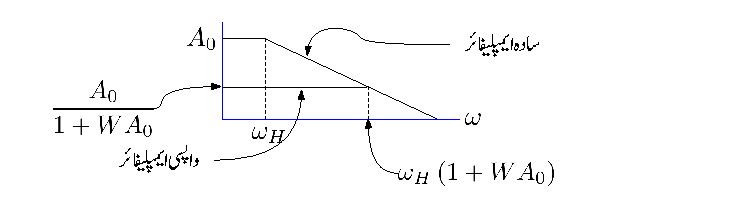
\includegraphics[scale=0.90]{feedbackGainBandwidthProductOctave}
\caption{دائرہ کارکردگی بالمقابل افزائش}
\label{شکل_واپسی_دائرہ_بالمقابل_افزائش}
\end{figure}
%=========================
\ابتدا{مثال}
ایک سادہ ایمپلیفائر کی درمیانی تعدد پر افزائش \عددیء{\SI{3000}{\volt \per \volt}} ہے جبکہ اس کی بلند انقطاعی تعدد \عددیء{\SI{500}{\hertz}} ہے۔اس میں واپسی اشارہ شامل کرتے ہوئے واپسی ایمپلیفائر حاصل کیا جاتا ہے۔اگر واپس کار کا مستقل \عددیء{W=0.01} ہو تب واپسی ایمپلیفائر کی درمیانی تعدد کی افزائش اور بلند انقطاعی تعدد کیا ہوں گے۔

حل:
\begin{align*}
A_{f0}&=\frac{3000}{1+3000 \times 0.01}=\SI{96.77}{\volt \per \volt}\\
f_H&=500 \times \left(1+3000 \times 0.01 \right)=\SI{15.5}{\kilo \hertz}
\end{align*}
\انتہا{مثال}
%==============
\حصہ{داخلی مزاحمت}
ہم نے دیکھا کہ منفی واپسی اشارے کی شمولیت سے افزائش \عددیء{M} گنا گھٹتی    ہے۔ اس حصے میں داخلی مزاحمت پر واپسی اشارے کے اثر کو دیکھا جائے گا۔

\جزوحصہ{واپسی برقی دباو ایمپلیفائر کا داخلی مزاحمت}
شکل \حوالہ{شکل_واپسی_دباو_ایمپلیفائر_تھیونن_مساوی} میں  داخلی جانب منفی واپسی  اشارہ \عددیء{V_f} شامل کرتے ہوئے  شکل \حوالہ{شکل_واپسی_دباو_ایمپلیفائر_داخلی_مزاحمت} حاصل ہوتا ہے۔فرق صرف اتنا ہے کہ موجودہ شکل میں \عددیء{R_s} کو ایمپلیفائر کا حصہ تصور کیا گیا ہے اور 
\begin{align} \label{مساوات_واپسی_افزائش_برقی_دباو_بمع_اشارہ_مزاحمت}
A_v'=A_v \left (\frac{R_i}{R_i + R_s} \right )
\end{align} 
رکھا گیا ہے۔یوں اشارے کی مزاحمت \عددیء{R_s} کو ایمپلیفائر کا حصہ تصور کرتے ہوئے افزائش برقی دباو کو \عددیء{A_v'} لکھا گیا ہے۔اس دور میں
\begin{align*}
V_o &=A_v'  V_i' \left (\frac{R_L}{R_o +R_L} \right) \\
&= A_v V_i' \left (\frac{R_i}{R_i+R_s} \right ) \left (\frac{R_L}{R_o+R_L} \right ) \\
\frac{V_o}{V_i'}&=A_v \left (\frac{R_i}{R_i+R_s} \right ) \left (\frac{R_L}{R_o+R_L} \right  )
\end{align*}
حاصل ہوتا ہے۔مساوات \حوالہ{مساوات_واپسی_افزائش_برقی_دباو_بمع_اشارہ_مزاحمت} اور مساوت \حوالہ{مساوات_واپسی_دباو_ایمپلیفائر_کی_افزائش} کے ساتھ موازنہ کرنے سے اس مساوات سے حاصل ہوتا ہے
\begin{align}  \label{مساوات_واپسی_دباو_افزائش_ب}
\frac{V_o}{V_i'}&=A_v' \left (\frac{R_L}{R_o+R_L} \right  ) =A_V
\end{align}
اس مساوات میں \عددیء{R_L \to \infty} کی صورت میں
\begin{align} \label{مساوات_واپسی_لامحدود_مزاحمت_پر_افزائش_برقی_دباو_ب}
\eval{A_V}_{R_L \to \infty} = A_v'
\end{align}
حاصل ہوتا ہے۔

واپسی اشارے کی عدم موجودگی میں
\begin{gather} \label{مساوات_واپسی_بغیر_واپسی_دباو_ایمپلیفائر_داخلی_مزاحمت}
\begin{aligned}
V_s =V_i'= I_i \left (R_i +R_s \right ) \\
R_i'=\frac{V_s}{I_i}=R_i+R_s
\end{aligned}
\end{gather}
حاصل ہوتا ہے جو کہ \عددیء{R_s} کو شامل کرتے ہوئے برقی دباو ایمپلیفائر کی کل داخلی مزاحمت \عددیء{R_i'} ہے۔آئیں اب واپسی اشارے کی شمولیت کے بعد \عددیء{\frac{V_s}{I_i}} حاصل کریں۔
\begin{align*}
V_s-V_f=I_i \left (R_s+R_i \right )  \\
V_s - W V_o = I_i \left (R_s+R_i \right )  \\
V_s-W A_V V_i'=I_i \left (R_s+R_i \right ) \\
V_s-W A_V I_i \left (R_s+R_i \right ) =I_i \left (R_s+R_i \right ) \\
V_s=\left(1+W A_V \right ) \left (R_s+R_i \right ) I_i
\end{align*}
اس مساوات میں تیسرے قدم پر مساوات \حوالہ{مساوات_واپسی_دباو_افزائش_ب} اور چوتھے قدم پر مساوات \حوالہ{مساوات_واپسی_بغیر_واپسی_دباو_ایمپلیفائر_داخلی_مزاحمت}  کا استعمال کیا گیا۔اس سے حاصل ہوتا ہے
\begin{gather}
\begin{aligned}\label{مساوات_واپسی_برقی_دباو_کی_داخلی_مزاحمت}
R_{if}' &=\frac{V_s}{I_i} \\
&=\left(1+W A_V \right ) \left (R_s+R_i \right ) \\
&=\left(1+W A_V \right ) R_i'
\end{aligned}
\end{gather}
اس مساوات کے مطابق منفی واپسی اشارے کی شمولیت  سے داخلی مزاحمت \عددیء{M} گنا بڑھ جاتا ہے۔

اس نتیجے کو یوں سمجھا جا سکتا ہے کہ واپسی اشارے کی عدم موجودگی میں اشارہ \عددیء{V_s} لاگو کرنے سے داخلی جانب برقی رو گزرتی ہے۔ان دونوں کی شرح کو \اصطلاح {داخلی مزاحمت}\فرہنگ{داخلی مزاحمت} کہتے ہیں۔منفی واپسی اشارے کے موجودگی میں داخلی جانب کل برقی دباو کم ہو کر \عددیء{(V_s-V_f)}  رہ جاتا ہے جس سے داخلی جانب برقی رو کی قیمت بھی کم ہو جاتی ہے۔یوں \عددیء{V_s} اور داخلی برقی رو کی شرح بڑھ جاتی ہے، جس سے داخلی مزاحمت بھی بڑھ جاتا ہے۔آپ دیکھ سکتے ہیں کہ برقی دباو کا واپسی اشارہ چاہے خارجی برقی دباو یا خارجی برقی رو سے حاصل کیا جائے، یہ  ہر صورت داخلی مزاحمت کو بڑھائے گا۔
\begin{figure}
\centering
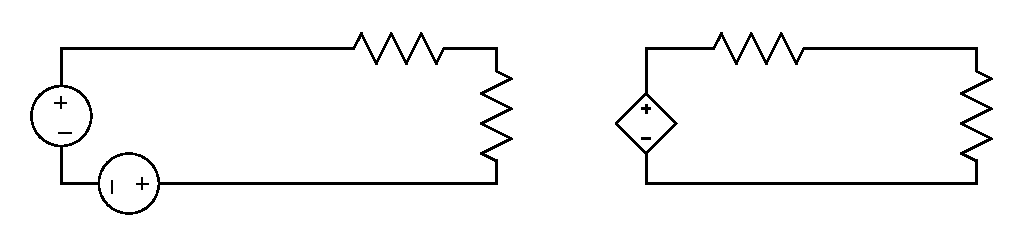
\includegraphics[scale=0.90]{voltageAmplifierInputResistance}
\caption{واپسی برقی دباو ایمپلیفائر کی داخلی مزاحمت}
\label{شکل_واپسی_دباو_ایمپلیفائر_داخلی_مزاحمت}
\end{figure}

مساوات \حوالہ{مساوات_واپسی_برقی_دباو_کی_داخلی_مزاحمت} میں \عددیء{R_s=0} پُر کرتے ہوئے
\begin{align}
R_{if}=\left(1+W A_V \right ) R_i
\end{align}
حاصل ہوتا ہے جہاں داخلی مزاحمت کو \عددیء{R_{if}} لکھ کر اس بات کی وضاحت کی گئی ہے کہ اس میں \عددیء{R_s=0} لیا گیا ہے۔

%========================
\جزوحصہ{واپسی برقی رو ایمپلیفائر کا داخلی مزاحمت}
شکل \حوالہ{شکل_واپسی_رو_ایمپلیفائر_نارٹن_مساوی} میں دکھائے برقی رو ایمپلیفائر میں داخلی جانب منفی واپسی اشارہ \عددیء{I_f} شامل کرتے ہوئے اسے یہاں شکل \حوالہ{شکل_واپسی_رو_ایمپلیفائر_داخلی_مزاحمت} میں دوبارہ دکھایا گیا ہے۔فرق صرف اتنا ہے کہ یہاں \عددیء{R_s} کو ایمپلیفائر کا حصہ تصور کیا گیا ہے اور
\begin{align} \label{مساوات_واپسی_داخلی_مزاحمت_شامل_کرتے_رو_افزائش}
A_i'=A_i \left (\frac{R_s}{R_s+R_i} \right )
\end{align}
رکھا گیا ہے۔اس دور میں 
\begin{align}
I_i'=I_s-I_f
\end{align}
کے برابر ہے۔

واپسی اشارے کی  عدم موجودگی (یعنی \عددیء{I_f =0}) کی صورت میں اشارہ \عددیء{I_s}  لاگو کرنے سے داخلی جانب  ہم لکھ سکتے ہیں
\begin{gather}
\begin{aligned}
I_i' &=I_s\\
V_i &= I_i' \left(\frac{R_s R_i}{R_s+R_i} \right ) =I_s \left(\frac{R_s R_i}{R_s+R_i} \right ) \\
R_i' &=\frac{V_i}{I_s}=\frac{R_s R_i}{R_s+R_i}
\end{aligned}
\end{gather}
جہاں \عددیء{R_s} کو شامل کرتے ہوئے، \عددیء{R_i'} بغیر واپسی ایمپلیفائر کی کل داخلی مزاحمت ہے۔اسی طرح شکل \حوالہ{شکل_واپسی_رو_ایمپلیفائر_داخلی_مزاحمت} میں 
\begin{align*}
I_o &= A_i'  I_i' \left( \frac{R_o}{R_o+R_L} \right )  \\
&=A_i  I_i' \left (\frac{R_s}{R_s+R_i} \right ) \left( \frac{R_o}{R_o+R_L} \right )  \\
 \frac{I_o}{I_i'} &=A_i \left (\frac{R_s}{R_s+R_i} \right ) \left( \frac{R_o}{R_o+R_L} \right )  
\end{align*}
حاصل ہوتا ہے جہاں دوسرے قدم پر مساوات \حوالہ{مساوات_واپسی_داخلی_مزاحمت_شامل_کرتے_رو_افزائش} کا استعمال کیا گیا ہے۔اس مساوات کے دائیں جانب کا مساوات \حوالہ{مساوات_واپسی_رو_ایمپلیفائر_کی_افزائش} کے ساتھ موازنہ کرنے سے حاصل ہوتا ہے
\begin{align} \label{مساوات_واپسی_رو_ایمپلیفائر_کی_افزائش_ب}
A_I=\frac{I_o}{I_i'}
\end{align}
واپسی اشارے کے موجودگی میں داخلی مزاحمت یوں حاصل ہو گا
\begin{align*}
I_i' &=I_s-I_f  \\
&=I_s -W I_o \\
&=I_s -W A_I I_i' \\
I_i' &=\frac{I_s}{1+W A_I}
\end{align*}
جہاں آخری قدم پر مساوات \حوالہ{مساوات_واپسی_رو_ایمپلیفائر_کی_افزائش_ب} کا استعمال کیا گیا۔اس صورت میں داخلی برقی دباو
\begin{align*}
V_i &= I_i' \left(\frac{R_s R_i}{R_s+R_i} \right ) \\
&=I_i' R_i' \\
& =\left(\frac{ I_s }{1+W A_I} \right) R_i' 
\end{align*}
حاصل ہوتا ہے جس سے 
\begin{align}\label{مساوات_واپسی_برقی_رو_کی_داخلی_مزاحمت}
R_{if}'=\frac{V_i}{I_s} =\frac{ R_i'}{1+W A_I}
\end{align}
حاصل ہوتا ہے۔اس مساوات کے تحت واپسی رو ایمپلیفائر  کا داخلی مزاحمت \عددیء{R_{if}'}  غیر واپسی ایمپلیفائر کے داخلی مزاحمت \عددیء{R_i'} سے \عددیء{M} گنا کم ہوتا ہے۔

اس حقیقت کو یوں سمجھا جا سکتا ہے کہ واپسی اشارے کے عدم موجودگی میں \عددیء{I_s}  داخلی مزاحمت \عددیء{R_i'} سے گزرتے ہوئے  \عددیء{V_i}  کو جنم دیتا ہے۔\عددیء{V_i} اور \عددیء{I_s} کی شرح کو \اصطلاح {داخلی مزاحمت}\فرہنگ{داخلی مزاحمت} کہتے ہیں۔واپسی اشارے کے موجودگی میں مزاحمت \عددیء{R_i'} سے گزرتی برقی رو کی قیمت کم ہو کر \عددیء{I_s -I_f} ہو جاتی ہے لہٰذا \عددیء{V_i}  کی قیمت بھی کم ہو جاتی ہے۔ یوں \عددیء{V_i} اور \عددیء{I_s} کی شرح بھی کم ہو جاتی ہے۔آپ دیکھ سکتے ہیں کہ \عددیء{I_f} چاہے خارجی برقی دباو \عددیء{V_o} یا خارجی برقی رو \عددیء{I_o} سے حاصل کیا جائے، اس کا داخلی کل مزاحمت پر ایک جیسا اثر ہوتا ہے یعنی کل داخلی مزاحمت کم ہوتا ہے۔ 
\begin{figure}
\centering
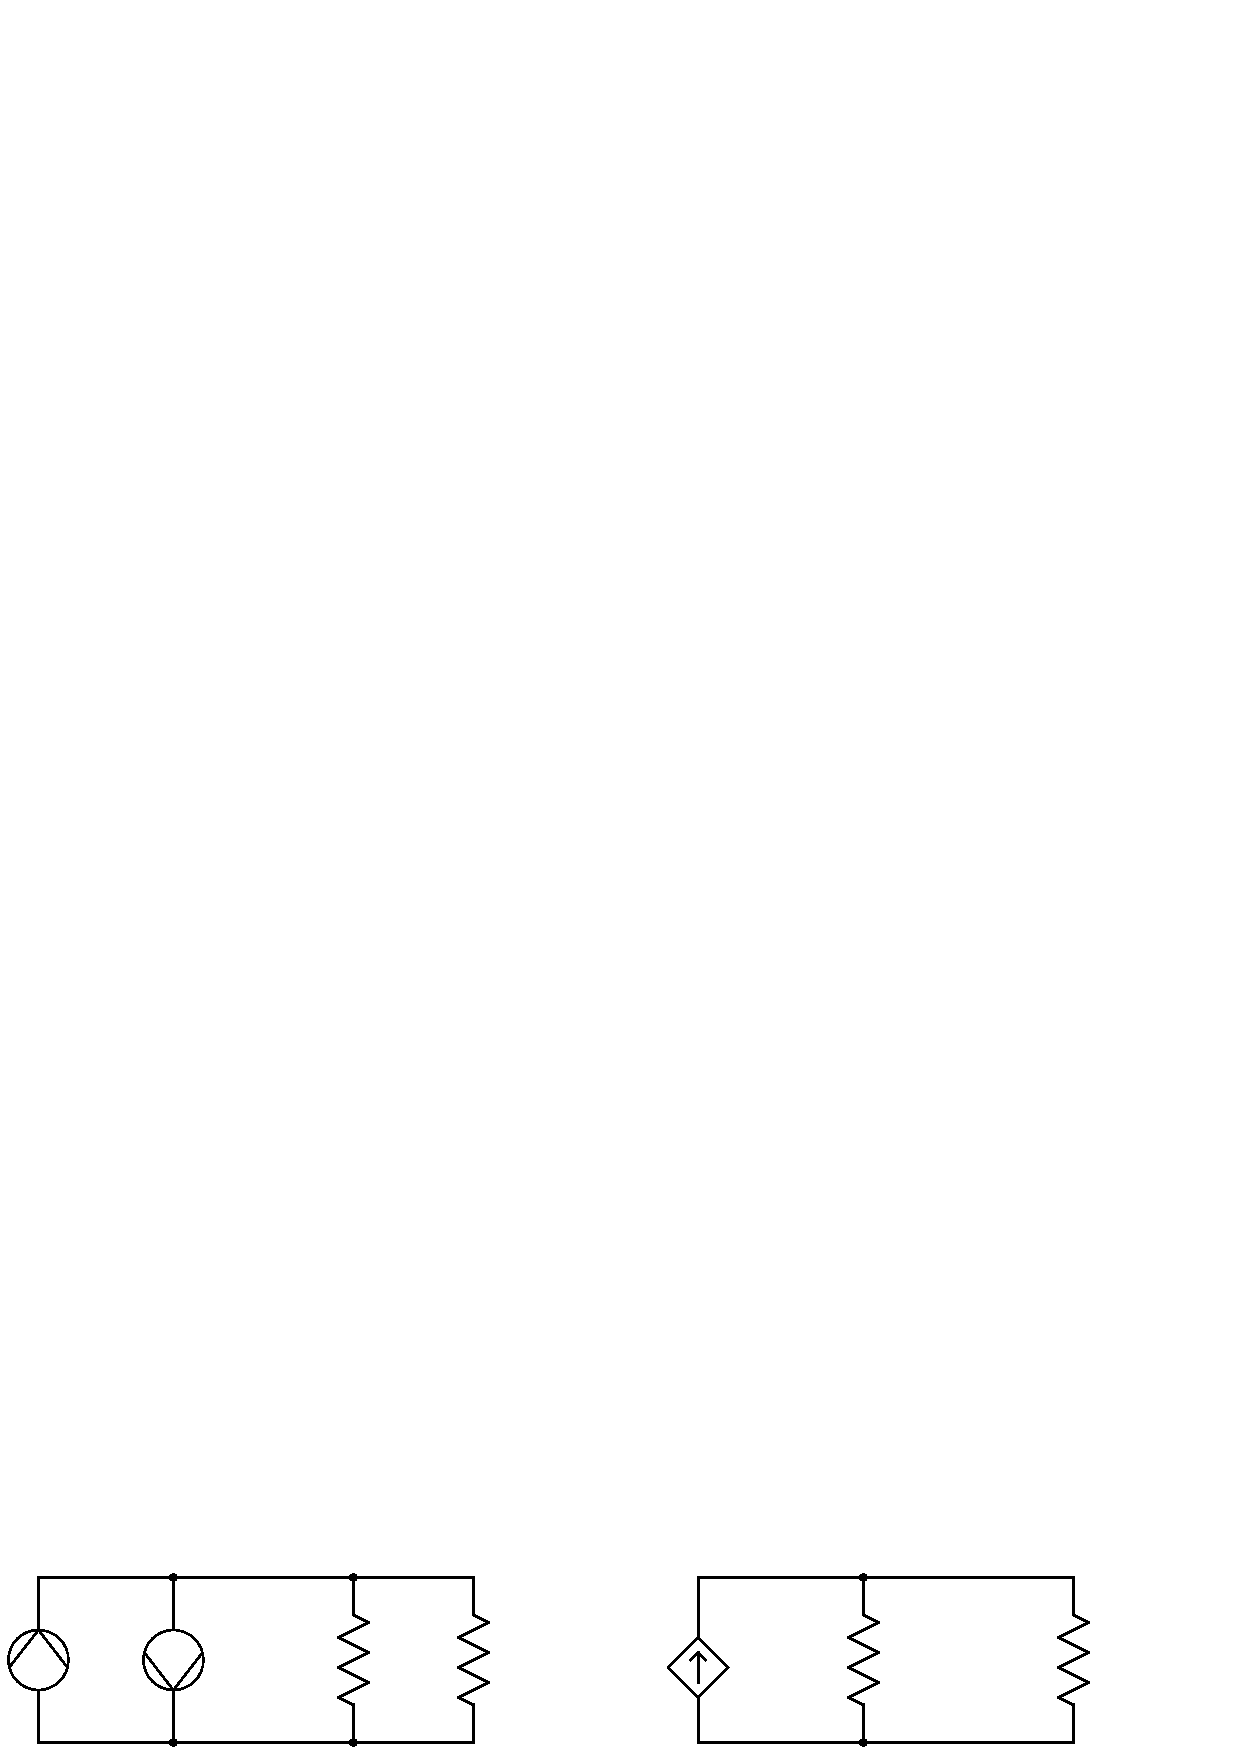
\includegraphics[scale=0.90]{currentAmplifierInputResistance}
\caption{واپسی برقی رو ایمپلیفائر کی داخلی مزاحمت}
\label{شکل_واپسی_رو_ایمپلیفائر_داخلی_مزاحمت}
\end{figure}

مساوات \حوالہ{مساوات_واپسی_برقی_رو_کی_داخلی_مزاحمت} میں \عددیء{R_s=0} پُر کرتے ہوئے
\begin{align}
R_{if}=\frac{ R_i}{1+W A_I}
\end{align}
حاصل ہوتا ہے جہاں داخلی مزاحمت کو \عددیء{R_{if}} لکھ کر اس بات کی وضاحت کی گئی ہے کہ اس میں \عددیء{R_s=0} لیا گیا ہے۔
%=============
\جزوحصہ{واپسی موصل نما ایمپلیفائر کا داخلی مزاحمت}
شکل \حوالہ{شکل_واپسی_موصلیت_نما_ایمپلیفائر_کا_مساوی_دور} میں واپسی اشارہ \عددیء{V_f} کی شمولیت اور
\begin{align} \label{مساوات_واپسی_موصلیت_نما_افزائش_بمع_اشارہ_مزاحمت}
A_g' = A_g \left( \frac{R_i}{R_s+R_i} \right )
\end{align}
تصور کرتے ہوئے یہاں شکل \حوالہ{شکل_واپسی_موصلیت_نما_ایمپلیفائر_داخلی_مزاحمت} میں دوبارہ دکھایا گیا ہے۔مزید یہ کہ یہاں \عددیء{R_s} کو ایمپلیفائر کا حصہ تصور کیا گیا ہے۔اس شکل کے لئے ہم لکھ سکتے ہیں
\begin{align*}
I_o&=A_g' V_i' \left (\frac{R_o}{R_o+R_L} \right ) \\
&=A_g V_i' \left (\frac{R_i}{R_s+R_i} \right ) \left (\frac{R_o}{R_o+R_L} \right ) \\
\frac{I_o}{V_i'}&=A_g \left (\frac{R_i}{R_s+R_i} \right ) \left (\frac{R_o}{R_o+R_L} \right )
\end{align*}
جہاں دوسرے قدم پر مساوات \حوالہ{مساوات_واپسی_موصلیت_نما_افزائش_بمع_اشارہ_مزاحمت}  کا استعمال کیا گیا۔مساوات \حوالہ{مساوات_واپسی_کل_موصلیت_نما} کے ساتھ موازنہ سے حاصل ہوتا ہے۔
\begin{align} \label{مساوات_واپسی_موصلیت_نما_افزائش_ب}
\frac{I_o}{V_i'}=A_G
\end{align}
واپسی اشارہ \عددیء{V_f} کے عدم موجودگی میں ہم \عددیء{R_s} کو شامل کرتے ہوئے کل داخلی مزاحمت \عددیء{R_i'} حاصل کرتے ہیں۔
\begin{align*}
V_i'=V_s =I_i \left(R_s+R_i \right) \\
R_i'=\frac{V_s}{I_i}=R_s+R_i
\end{align*}
آئیں اب واپسی اشارے کے موجودگی میں کل داخلی مزاحمت \عددیء{R_{if}'} حاصل کریں۔ 
\begin{gather} \label{مساوات_واپسی_داخلی_دباو_بالمقابل_اشارہ}
\begin{aligned}
V_i' &=V_s-V_f \\
&=V_s-W I_o \\
&=V_s-W A_G V_i'\\
V_i'&=\frac{V_s}{1+W A_G}
\end{aligned}
\end{gather}
تیسرے قدم پر مساوات \حوالہ{مساوات_واپسی_موصلیت_نما_افزائش_ب} کا استعمال کیا گیا۔ اس مساوات کو 
\begin{align}
V_i'=I_i \left( R_s+R_i\right)
\end{align}
میں ڈالتے  ہیں
\begin{align*}
\frac{V_s}{1+W A_G}=I_i \left( R_s+R_i\right)
\end{align*}
جس سے حاصل ہوتا ہے
\begin{gather}
\begin{aligned}\label{مساوات_واپسی_موصل_نما_کی_داخلی_مزاحمت}
R_{if}'&=\frac{V_s}{I_i}=\left ({R_s+R_i} \right ) \left ({1+W A_G} \right) \\
&={R_i'} \left({1+W A_G} \right )
\end{aligned}
\end{gather}
اس مساوات کے مطابق واپسی اشارے کے موجودگی میں کل داخلی مزاحمت \عددیء{R_{if}'} کی قیمت واپسی اشارے کے عدم موجودگی میں کل داخلی مزاحمت \عددیء{R_i} کے \عددیء{M} گنا ہے۔
\begin{figure}
\centering
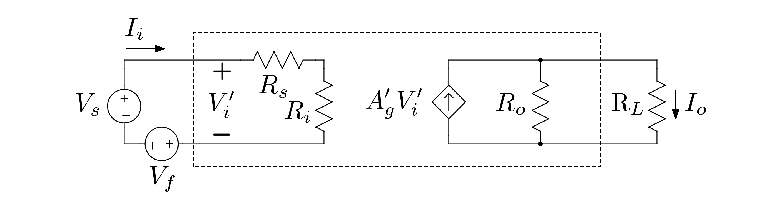
\includegraphics[scale=0.90]{transconductanceAmplifierInputResistance}
\caption{واپسی موصل نما ایمپلیفائر کی داخلی مزاحمت}
\label{شکل_واپسی_موصلیت_نما_ایمپلیفائر_داخلی_مزاحمت}
\end{figure}

مساوات \حوالہ{مساوات_واپسی_موصل_نما_کی_داخلی_مزاحمت} میں \عددیء{R_s=0} پُر کرتے ہوئے
\begin{align}
R_{if}={R_i} \left({1+W A_G} \right )
\end{align}
حاصل ہوتا ہے جہاں داخلی مزاحمت کو \عددیء{R_{if}} لکھ کر اس بات کی وضاحت کی گئی ہے کہ اس میں \عددیء{R_s=0} لیا گیا ہے۔
%===================
\جزوحصہ{واپسی مزاحمت نما ایمپلیفائر کا داخلی مزاحمت}
شکل \حوالہ{شکل_واپسی_مزاحمت_نما_ایمپلیفائر_کا_مساوی_دور} میں واپسی اشارہ \عددیء{V_f} کی شمولیت اور
\begin{align} \label{مساوات_واپسی_مزاحمت_نما_افزائش_بمع_اشارہ_مزاحمت}
A_r' = A_r \left( \frac{R_s}{R_s+R_i} \right )
\end{align}
تصور کرتے ہوئے یہاں شکل \حوالہ{شکل_واپسی_مزاحمت_نما_ایمپلیفائر_داخلی_مزاحمت} میں دوبارہ دکھایا گیا ہے۔مزید یہ کہ یہاں \عددیء{R_s} کو ایمپلیفائر کا حصہ تصور کیا گیا ہے۔اس شکل کے لئے ہم لکھ سکتے ہیں
\begin{align*}
V_o&=A_r' I_i' \left (\frac{R_L}{R_o+R_L} \right )\\
&=A_r  I_i' \left( \frac{R_s}{R_s+R_i} \right ) \left (\frac{R_L}{R_o+R_L} \right ) \\
\frac{V_o}{I_i'}&=A_r  \left( \frac{R_s}{R_s+R_i} \right ) \left (\frac{R_L}{R_o+R_L} \right )
\end{align*}
جہاں دوسرے قدم پر مساوات \حوالہ{مساوات_واپسی_مزاحمت_نما_افزائش_بمع_اشارہ_مزاحمت} کا استعمال کیا گیا ہے۔مساوات \حوالہ{مساوات_واپسی_کل_مزاحمت_نما} کے ساتھ موازنہ  کرتے ہوئے مندرجہ بالا مساوات سے حاصل ہوتا ہے۔
\begin{align} \label{مساوات_واپسی_مزاحمت_نما_افزائش_ب}
\frac{V_o}{I_i'}=A_R
\end{align}
واپسی اشارے کے عدم موجودگی میں \عددیء{I_i'=I_s} ہو تا ہے لہٰذا  داخلی مزاحمت \عددیء{R_i'} یوں حاصل ہوتا ہے 
\begin{gather}
\begin{aligned}
V_i &=I_i' \left (\frac{R_s R_i}{R_s +R_i} \right ) \\
&=I_s \left (\frac{R_s R_i}{R_s +R_i} \right ) \\
R_i'&=\frac{V_i}{I_s}= \left (\frac{R_s R_i}{R_s +R_i} \right )
\end{aligned}
\end{gather}
واپسی اشارے کے موجودگی میں
\begin{align*}
I_i'&=I_s-I_f\\
&=I_s-W V_o \\
&=I_s-W A_R I_i'\\
I_i'&=\frac{I_s}{1+W A_R}
\end{align*}
اس مساوات کو
\begin{align*}
V_i &=I_i' \left(\frac{R_s R_i}{R_s +R_i} \right )
\end{align*}
میں استعمال کرتے حاصل ہوتا ہے
\begin{align*}
V_i &= \left (\frac{I_s}{1+W A_R} \right ) \left(\frac{R_s R_i}{R_s +R_i} \right ) 
\end{align*}
جس سے واپسی اشارے کے موجودگی میں کل داخلی مزاحمت \عددیء{R_{if}'} یوں حاصل ہوتا ہے۔
\begin{gather}
\begin{aligned}\label{مساوات_واپسی_مزاحمت_نما_کی_داخلی_مزاحمت}
R_{if}'&=\frac{V_i}{I_s} = \left (\frac{1}{1+W A_R} \right ) \left(\frac{R_s R_i}{R_s +R_i} \right ) \\
&=\frac{R_i'}{1+W A_R}
\end{aligned}
\end{gather}
اس مساوات کے تحت واپسی اشارے کے موجودگی میں کل داخلی مزاحمت \عددیء{R_{if}'} کی قیمت واپسی اشارے کے عدم موجودگی میں کل داخلی مزاحمت \عددیء{R_i'} سے \عددیء{M} گنا کم ہوتا ہے۔
\begin{figure}
\centering
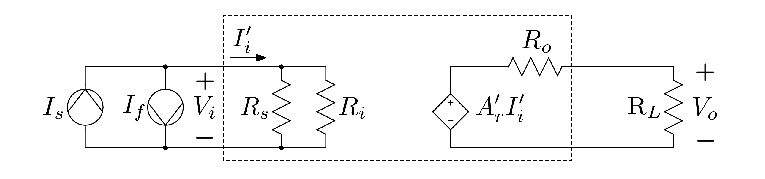
\includegraphics[scale=0.90]{transresistanceAmplifierInputResistance}
\caption{واپسی مزاحمت نما ایمپلیفائر کی داخلی مزاحمت}
\label{شکل_واپسی_مزاحمت_نما_ایمپلیفائر_داخلی_مزاحمت}
\end{figure}

مساوات \حوالہ{مساوات_واپسی_مزاحمت_نما_کی_داخلی_مزاحمت} میں \عددیء{R_s=0} پُر کرتے ہوئے
\begin{align}
R_{if}=\frac{R_i}{1+W A_R}
\end{align}
حاصل ہوتا ہے جہاں داخلی مزاحمت کو \عددیء{R_{if}} لکھ کر اس بات کی وضاحت کی گئی ہے کہ اس میں \عددیء{R_s=0} لیا گیا ہے۔
%==============
\حصہ{خارجی مزاحمت}
اس حصے میں خارجی مزاحمت پر واپسی اشارے کے اثر کو دیکھا جائے گا۔

\جزوحصہ{واپسی برقی دباو ایمپلیفائر کا خارجی مزاحمت}
شکل \حوالہ{شکل_واپسی_دباو_ایمپلیفائر_داخلی_مزاحمت} میں \عددیء{R_L} کو منقطع کرتے ہوئے، \عددیء{V_s=0} رکھ \حاشیہد{برقی دباو کو صفر کرنے کی خاطر اسے قصر دور کیا جاتا ہے} کر خارجی جانب برقی دباو \عددیء{V_t} لاگو کرتے ہیں۔\عددیء{V_t} اور \عددیء{I_t} کی شرح اس ایمپلیفائر کا خارجی مزاحمت \عددیء{R_{of}} ہو گا۔شکل \حوالہ{شکل_واپسی_برقی_دباو_ایمپلیفائر_خارجی_مزاحمت} میں ایسا دکھایا گیا ہے جہاں سے ہم لکھ سکتے ہیں
\begin{align*}
I_t&=\frac{V_t-A_v' V_i'}{R_o}\\
&=\frac{V_t +A_v' V_f}{R_o} \\
&=\frac{V_t+A_v' W V_t}{R_o}
\end{align*}
اور یوں واپسی اشارے کے موجودگی میں خارجی مزاحمت یوں حاصل ہوتا ہے
\begin{align}
R_{of}=\frac{V_t}{I_t}=\frac{R_o}{1+W A_v'}
\end{align}
اگر \عددیء{R_L} کو بھی شامل کیا جائے تب چونکہ \عددیء{R_L} اور \عددیء{R_{of}}  متوازی جڑے ہیں لہٰذا اس صورت کل خارجی مزاحمت \عددیء{R_of'} یوں حاصل ہو گی
\begin{align*}
R_{of'}&=\frac{R_{of} R_L}{R_{of}+R_L}=\frac{\left (\frac{R_o}{1+W A_v'}\right ) R_L} {\left (\frac{R_o}{1+W A_v'} \right )+R_L}\\
&=\frac{\frac{R_o R_L}{1+W A_v'}}{\frac{R_o+R_L \left (1+W A_v' \right )}{1+W A_v'}}=\frac{R_o R_L}{R_o +R_L \left ( 1+W A_v'\right )}\\
&=\frac{R_o R_L}{R_o +R_L + W A_v' R_L}=\frac{R_o R_L}{\left (R_o +R_L \right ) \left (1 + \frac{W A_v' R_L}{R_o+R_L} \right )}\\
&=\frac{\frac{R_o R_L}{R_o+R_L}}{1+\frac{W A_v' R_L}{R_o+R_L}}
\end{align*}
\عددیء{\frac{R_o R_L}{R_o+R_L}} دراصل \عددیء{R_o} اور \عددیء{R_L} کا مساوی متوازی مزاحمت ہے جسے \عددیء{R_o'} لکھتے ہوئے اور \عددیء{\frac{A_v' R_L}{R_o+R_L}} کو \عددیء{A_V} لکھتے ہوئے مندرجہ بالا مساوات سے حاصل ہوتا ہے
\begin{align}
R_{of'}=\frac{R_o'}{1+W A_V}
\end{align}
مزید لا محدود مزاحمتی بوجھ یعنی \عددیء{R_L \to \infty} پر
\begin{align} \label{مساوات_واپسی_لامحدود_بار_مزاحمت__پر_مزاحمت}
\left. R_{of}' \right|_{R_L \to \infty}=\left. \frac{R_{of} R_L}{R_{of}+R_L} \right|_{R_L \to \infty} = R_{of}
\end{align}
ہی حاصل ہوتا ہے
\begin{figure}
\centering
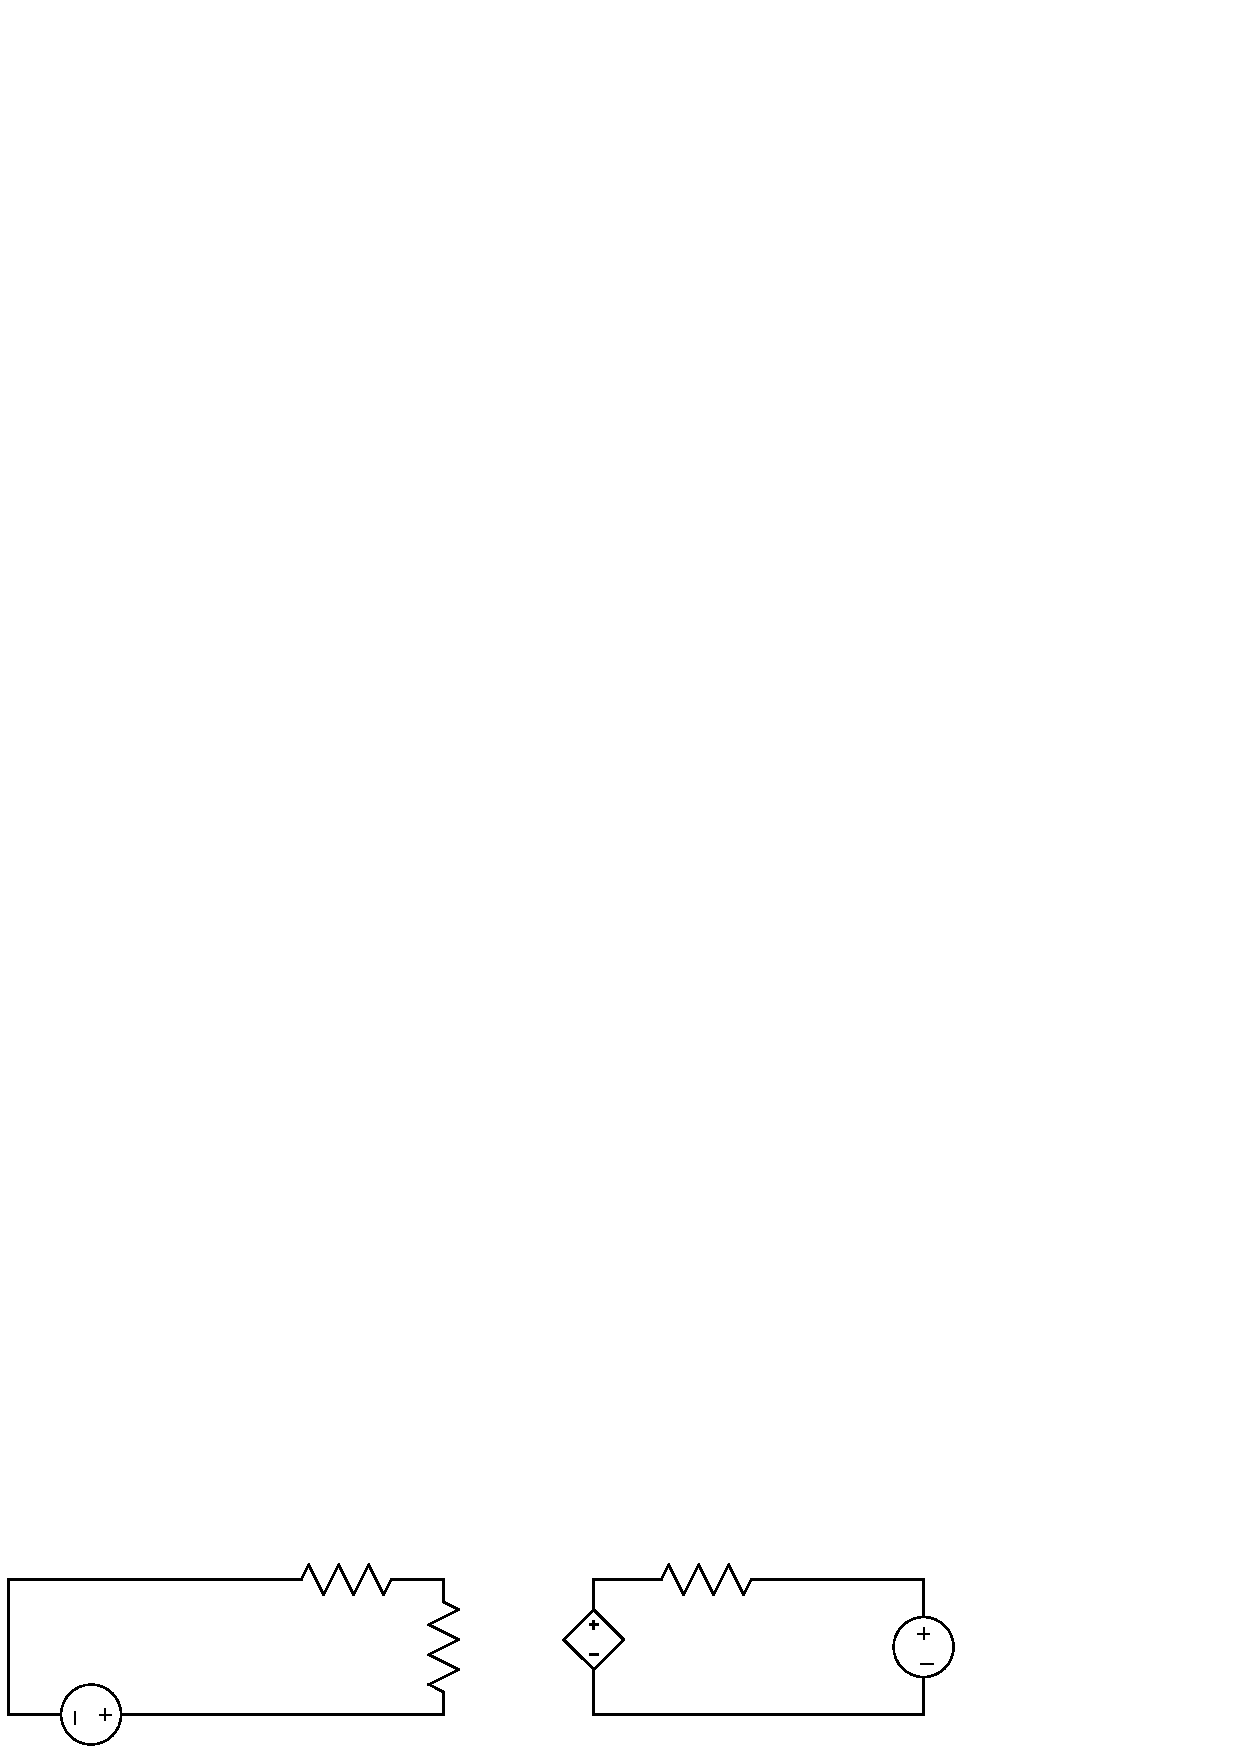
\includegraphics[scale=0.90]{voltageAmplifierOutputResistance}
\caption{واپسی برقی دباو ایمپلیفائر کا خارجی مزاحمت}
\label{شکل_واپسی_برقی_دباو_ایمپلیفائر_خارجی_مزاحمت}
\end{figure}
%==================
\جزوحصہ{واپسی برقی رو ایمپلیفائر کا خارجی مزاحمت}
شکل \حوالہ{شکل_واپسی_رو_ایمپلیفائر_داخلی_مزاحمت} میں \عددیء{R_L} کو منقطع کرتے ہوئے، \عددیء{I_s=0} رکھ \حاشیہد{برقی رو کو صفر کرنے کی خاطر اسے کھلے دور کیا جاتا ہے} کر خارجی جانب برقی دباو \عددیء{V_t} لاگو کرتے ہیں۔\عددیء{V_t} اور \عددیء{I_t} کی شرح اس ایمپلیفائر کا خارجی مزاحمت \عددیء{R_{of}} ہو گا۔شکل \حوالہ{شکل_واپسی_برقی_رو_ایمپلیفائر_خارجی_مزاحمت} میں ایسا دکھایا گیا ہے جہاں سے ہم لکھ سکتے ہیں
\begin{align*}
V_t&=\left(I_t+A_i' I_i' \right ) R_o \\
&=\left(I_t-A_i' I_f \right ) R_o \\
&=\left(I_t-A_i' W I_o \right ) R_o 
\end{align*}
جیسا شکل میں دکھایا گیا ہے  \عددیء{I_t=-I_o} ہے لہٰذا مندرجہ بالا مساوات کو یوں لکھ سکتے ہیں
\begin{align*}
V_t=\left (I_t +A_i' W I_t\right ) R_o
\end{align*}
جس سے \عددیء{R_{of}} یوں حاصل ہوتا ہے
\begin{align}
R_{of}=\frac{V_t}{I_t}=R_o \left (1+W A_i' \right )
\end{align}
مزاحمتی بوجھ \عددیء{R_L} مزاحمت \عددیء{R_{of}} کے متوازی جڑا ہے لہٰذا اس کے شمولیت سے کل خارجی مزاحمت \عددیء{R_{of}'}  یوں حاصل کرتے ہیں۔
\begin{align*}
R_{of}'&=\frac{R_{of} R_L}{R_{of}+R_L}=\frac{R_o \left (1+W A_i'\right ) R_L}{R_o \left (1+W A_i'\right )+R_L}\\
&=\frac{\left (1+W A_i'\right )R_o R_L}{R_o+W A_i' R_o+R_L}=\frac{\left (1+W A_i'\right )R_o R_L}{R_o+R_L+W A_i' R_o}\\
&=\frac{\left (1+W A_i'\right )R_o R_L}{\left (R_o+R_L\right)+W A_i' R_o}=\frac{\left (1+W A_i'\right )R_o R_L}{\left (R_o+R_L\right) \left (1+ \frac{W A_i' R_o}{R_o+R_L}\right )} \\
&=\left(\frac{R_o R_L}{R_o+R_L} \right) \frac{\left (1+W A_i' \right )}{\left (1+W \frac{A_i' R_o}{R_o+R_L} \right )}
\end{align*}
\عددیء{R_o}  اور \عددیء{R_L} متوازی جوڑنے سے \عددیء{\frac{R_o R_L}{R_o+R_L}}  حاصل ہو گا۔اس کو  \عددیء{R_o'} اور \عددیء{\frac{A_i' R_o}{R_o+R_L}}  کو \عددیء{A_I} لکھتے ہوئے حاصل ہوتا ہے
\begin{align} 
R_{of}'=R_o' \frac{\left (1+W A_i'\right )}{\left (1+ W A_I\right )}
\end{align}
%
\begin{figure}
\centering
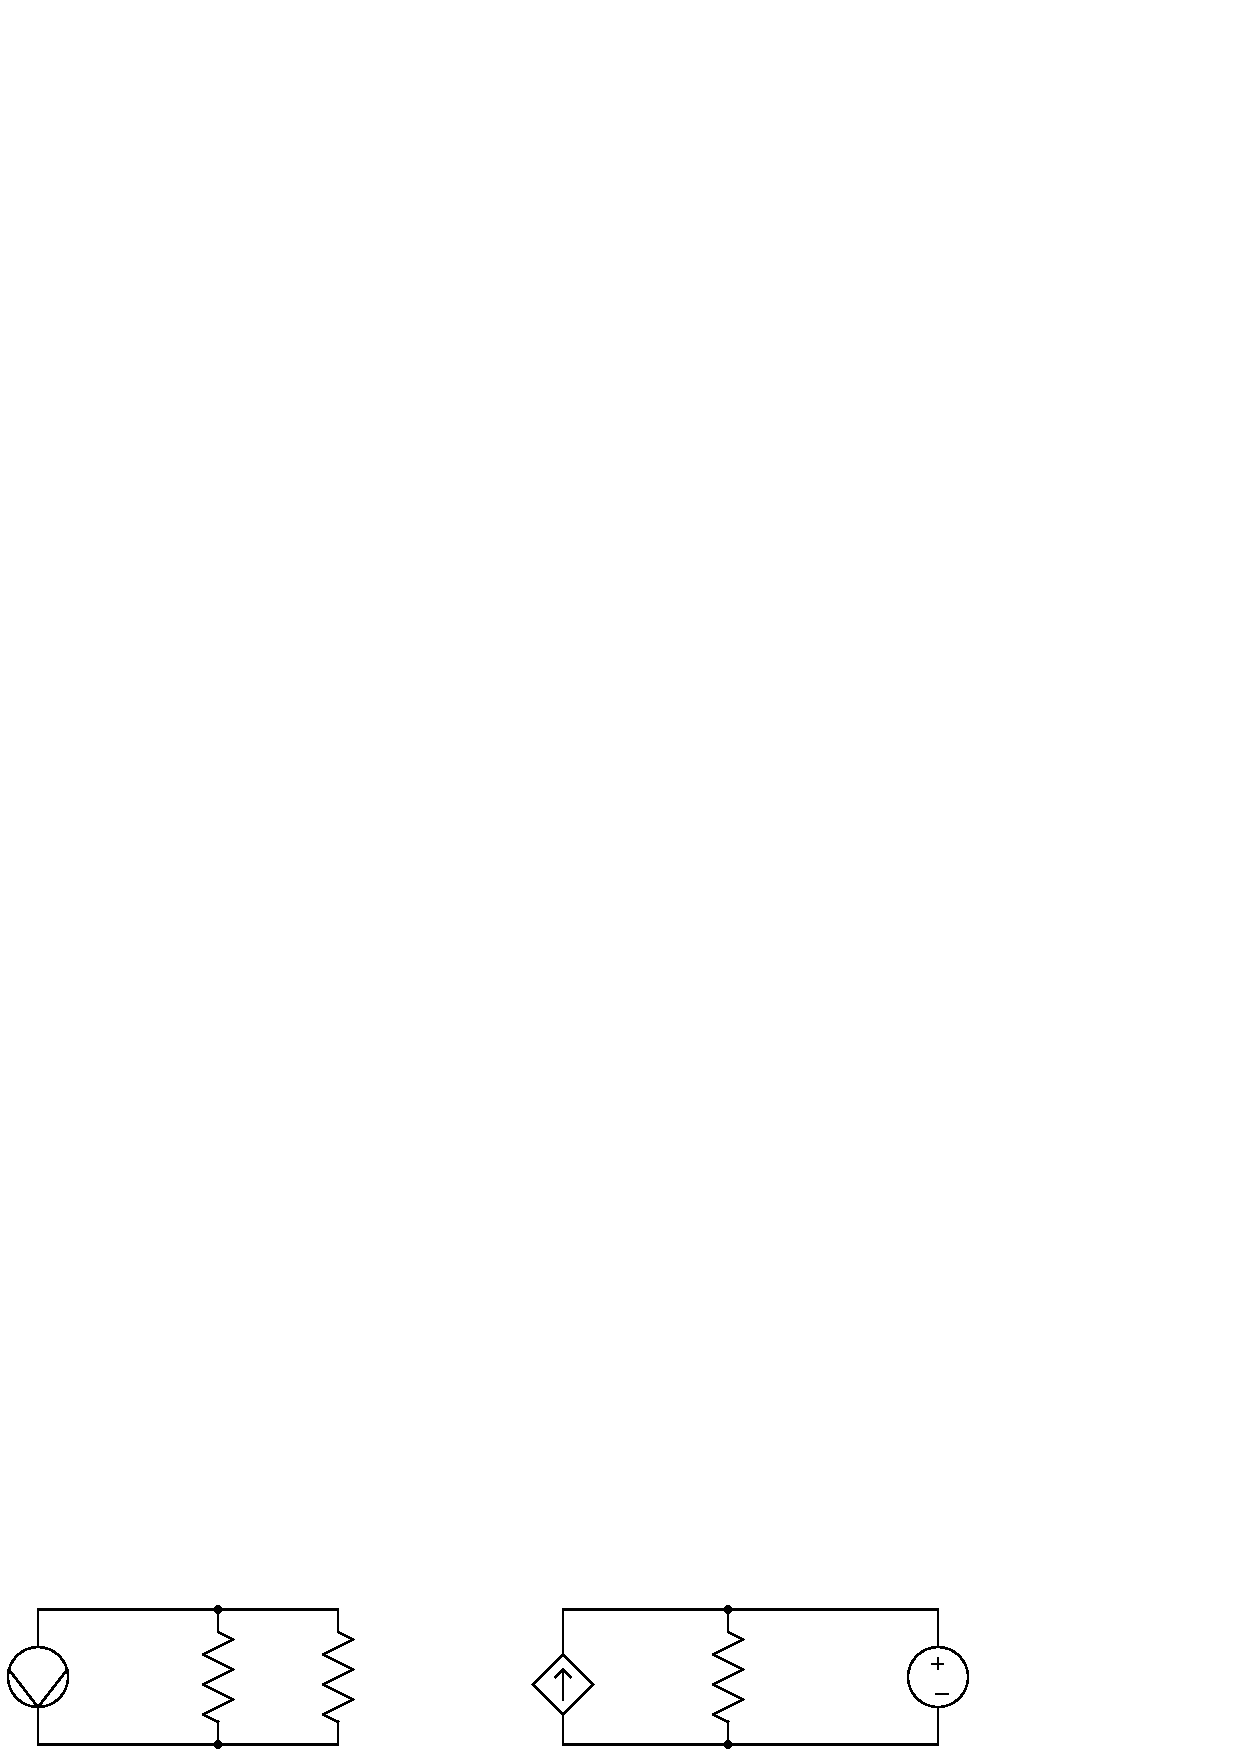
\includegraphics[scale=0.90]{currentAmplifierOutputResistance}
\caption{واپسی برقی رو ایمپلیفائر کا خارجی مزاحمت}
\label{شکل_واپسی_برقی_رو_ایمپلیفائر_خارجی_مزاحمت}
\end{figure}
%======================


\جزوحصہ{واپسی موصل نما ایمپلیفائر کا خارجی مزاحمت}
شکل \حوالہ{شکل_واپسی_موصلیت_نما_ایمپلیفائر_داخلی_مزاحمت} میں \عددیء{R_L} کو منقطع کرتے ہوئے، \عددیء{V_s=0} رکھ \حاشیہد{برقی دباو کو صفر کرنے کی خاطر اسے قصر دور کیا جاتا ہے} کر خارجی جانب برقی دباو \عددیء{V_t} لاگو کرتے ہیں۔\عددیء{V_t} اور \عددیء{I_t} کی شرح اس ایمپلیفائر کا خارجی مزاحمت \عددیء{R_{of}} ہو گا۔شکل \حوالہ{شکل_واپسی_موصلیت_نما_ایمپلیفائر_خارجی_مزاحمت} میں ایسا دکھایا گیا ہے جہاں سے ہم لکھ سکتے ہیں
\begin{align*}
V_t &=\left (I_t+A_g' V_i' \right) R_o \\
&=\left (I_t-A_g' V_f \right) R_o \\
&=\left (I_t- A_g' W I_o \right) R_o \\
&=\left (I_t+ A_g' W I_t \right) R_o
\end{align*}
جہاں دوسرے قدم پر \عددیء{V_i'=-V_f} اور چوتھے قدم پر \عددیء{I_o=-I_t} کا استعمال کیا گیا ہے۔یوں کل خارجی مزاحمت \عددیء{R_{of}}  کی قیمت یوں حاصل ہوتی ہے۔
\begin{align}
R_{of}=\frac{V_t}{I_t}=R_o \left (1+W A_g' \right )
\end{align}
اگر \عددیء{R_L} کو بھی شامل کیا جائے تب کل خارجی مزاحمت کو \عددیء{R_{of}'} لکھتے ہوئے
\begin{align*}
R_{of}' &=\frac{R_{of} R_L}{R_{of}+R_L}=\frac{R_o R_L \left (1+W A_g' \right )}{R_o \left (1+W A_g' \right )+R_L}\\
&=\frac{R_o R_L \left (1+W A_g' \right )}{R_o +R_o W A_g' +R_L}=\frac{R_o R_L \left (1+W A_g' \right )}{ \left (R_o+R_L \right )\left(1+\frac{R_o W A_g'}{R_o+R_L} \right)} \\
&=\left (\frac{R_o R_L}{R_o+R_L} \right ) \left ( \frac{1+W A_g'}{1+\frac{R_o  A_g' W}{R_o+R_L}}\right )
\end{align*}
اس مساوات میں \عددیء{\frac{R_o R_L}{R_o+R_L}} کو \عددیء{R_o'} لکھتے ہوئے اور \عددیء{\frac{R_o A_g'}{R_o+R_L}} کو \عددیء{A_G} لکھتے ہوئے حاصل ہوتا ہے
\begin{align}
R_{of}'=R_o'  \left (\frac{1+W A_g'}{1+W A_G}\right )
\end{align}
%
\begin{figure}
\centering
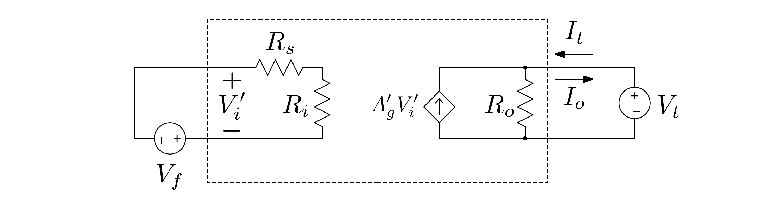
\includegraphics[scale=0.90]{transconductanceAmplifierOutputResistance}
\caption{واپسی موصل نما ایمپلیفائر کا خارجی مزاحمت}
\label{شکل_واپسی_موصلیت_نما_ایمپلیفائر_خارجی_مزاحمت}
\end{figure}

\جزوحصہ{واپسی مزاحمت نما ایمپلیفائر کا خارجی مزاحمت}
شکل \حوالہ{شکل_واپسی_مزاحمت_نما_ایمپلیفائر_داخلی_مزاحمت} میں \عددیء{R_L} کو منقطع کرتے ہوئے، \عددیء{I_s=0} رکھ \حاشیہد{برقی رو کو صفر کرنے کی خاطر اسے کھلے دور کیا جاتا ہے} کر خارجی جانب برقی دباو \عددیء{V_t} لاگو کرتے ہیں۔\عددیء{V_t} اور \عددیء{I_t} کی شرح اس ایمپلیفائر کا خارجی مزاحمت \عددیء{R_{of}} ہو گا۔شکل \حوالہ{شکل_واپسی_مزاحمت_نما_ایمپلیفائر_خارجی_مزاحمت} میں ایسا دکھایا گیا ہے جہاں سے ہم لکھ سکتے ہیں
\begin{align*}
I_t &=\frac{V_t-A_r' I_i'}{R_o} \\
&=\frac{V_t+A_r' I_f}{R_o} \\
&=\frac{V_t+A_r' W V_o}{R_o} \\
&=\frac{V_t+A_r' W V_t}{R_o}
\end{align*}
جہاں دوسرے قدم پر \عددیء{I_i'=-I_f} کا استعمال اور چوتھے قدم پر \عددیء{V_o=V_t} کا استعمال کیا گیا ہے۔یوں کل خارجی مزاحمت \عددیء{R_{of}} کو یوں حاصل کیا جا سکتا ہے۔
\begin{align}
R_{of}=\frac{V_t}{I_t}=\frac{R_o}{1+W A_r'}
\end{align}
اگر \عددیء{R_L} کو بھی شامل کیا جائے تب کل خارجی مزاحمت \عددیء{R_{of}'} کو یوں حاصل کیا جائے گا۔
\begin{align*}
R_{of}' &=\frac{R_{of} R_L}{R_{of}+R_L}=\frac{\left(\frac{R_o R_L}{1+W A_r'} \right)}{\left(\frac{R_o}{1+W A_r'}+R_L \right)}\\
&=\frac{\left(\frac{R_o R_L}{1+W A_r'} \right)}{\left(\frac{R_o+R_L \left(1+W A_r' \right )}{1+W A_r'} \right)}=\frac{R_o R_L}{R_o+R_L \left (1+W A_r'  \right)} \\
&=\frac{R_o R_L}{R_o+R_L +W A_r' R_L}=\frac{R_o R_L}{\left(R_o+R_L \right ) \left(1+ \frac{W A_r' R_L}{R_o+R_L}\right)}\\
&=\left(\frac{R_o R_L}{R_o+R_L} \right) \left (\frac{1}{1+\frac{W A_r' R_L}{R_o+R_L}} \right)
\end{align*}
اس مساوات میں \عددیء{\frac{R_o R_L}{R_o+R_L}} کو \عددیء{R_o'} لکھتے ہوئے اور \عددیء{\frac{A_r' R_L}{R_o+R_L}} کو \عددیء{A_R} لکھتے ہوئے حاصل ہوتا ہے
\begin{align}
R_{of}'=\frac{R_o'}{1+W A_R}
\end{align}
%
\begin{figure}
\centering
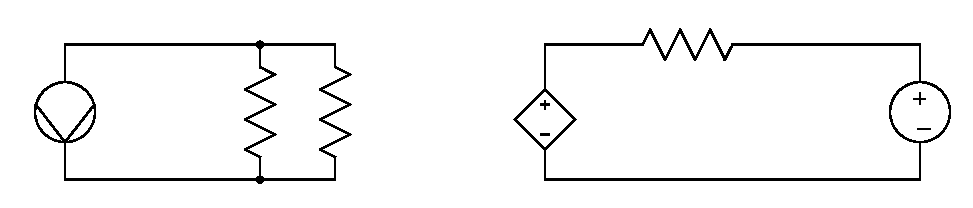
\includegraphics[scale=0.90]{transresistanceAmplifierOutputResistance}
\caption{واپسی مزاحمت نما ایمپلیفائر کا خارجی مزاحمت}
\label{شکل_واپسی_مزاحمت_نما_ایمپلیفائر_خارجی_مزاحمت}
\end{figure}
%===============================

جدول \حوالہ{جدول_واپسی_ایمپلیفائر_مختلف_تفاعل} میں ان نتائج کو پیش کیا گیا ہے۔

\begin{table} [h]
\caption{واپسی ایمپلیفائر کے داخلی اور خارجی مزاحمت}
\label{جدول_واپسی_ایمپلیفائر_مختلف_تفاعل}
\centering
\begin{tabular}{ r  l l}
\toprule
ایمپلیفائر کی قسم  & داخلی مزاحمت  & خارجی مزاحمت\\
\midrule
برقی دباو & \عددیء{R_{if}'=R_i'\left(1+W A_V \right)}  &\عددیء{R_{of}=\displaystyle \frac{R_o}{1+W A_{v}'}}  \\[5mm]
برقی رو & \عددیء{R_{if}'=\displaystyle\frac{R_i'}{1+W A_I}}&\عددیء{R_{of}=R_o \left(1+W A_i' \right)}   \\[5mm]
موصل نما  & \عددیء{R_{if}'=R_i'\left(1+W A_G \right)} &\عددیء{R_{of}=R_o \left(1+W A_g' \right)}    \\[5mm]
مزاحمت نما & \عددیء{R_{if}'=\displaystyle\frac{R_i'}{1+W A_R}} &\عددیء{R_{of}=\displaystyle\frac{R_o}{1+W A_r'}}  \\[3mm]
\bottomrule
\end{tabular}
\end{table}

برقی دباو ایمپلیفائر کا داخلی مزاحمت زیادہ سے زیادہ جبکہ اس کا خارجی مزاحمت کم سے کم درکار ہوتا ہے۔اس جدول سے آپ دیکھ سکتے ہیں کہ  واپسی اشارے کی شمولیت سے برقی دباو ایمپلیفائر کا داخلی مزاحمت بڑھتا ہے جبکہ اس کا خارجی مزاحمت گھٹتا ہے۔جہاں ایمپلیفائر کا داخلی اشارہ برقی دباو ہو وہاں زیادہ سے زیادہ داخلی مزاحمت درکار ہوتا ہے جبکہ اس کے برعکس جہاں داخلی اشارہ برقی رو ہو وہاں کم سے کم داخلی مزاحمت درکار ہوتا ہے۔اسی طرح جہاں خارجی اشارہ برقی دباو کا ہو وہاں کم سے کم خارجی مزاحمت درکار ہوتا ہے جبکہ خارجی اشارہ برقی رو ہونے کی صورت میں زیادہ سے زیادہ خارجی مزاحمت درکار ہوتا ہے۔جدول سے آپ دیکھ سکتے ہیں کہ تمام صورتوں میں واپسی اشارے کی شمولیت سے داخلی اور خارجی مزاحمت بہتر ہوتے ہیں۔سوال  \حوالہ{سوال_واپسی_برقی_دباو_ایمپلیفائر} تا سوال \حوالہ{سوال_واپسی_مزاحمت_نما_ایمپلیفائر} انہیں حقائق کو اجاگر کرتے ہیں۔ ان سوالات میں آپ یہ بھی دیکھیں گے کہ \عددیء{W A \gg 1} کی صورت میں \عددیء{A_{f} \approx \tfrac{1}{W}}  لیا جا سکتا ہے۔

%===============================
\حصہ{واپسی ایمپلیفائر کے جماعت بندی کی مثالیں}
کسی بھی واپسی ایمپلیفائر کے جماعت بندی اس کے داخلی جانب مساوات \حوالہ{مساوات_واپسی_ایمپلیفائر_کے_جماعت_بندی} کے طرز کے مساوات سے کی جاتی ہے۔ایسے مساوات میں \عددیء{X_s} اور \عددیء{X_o} سے جدول \حوالہ{جدول_واپسی_ایمپلیفائر_جماعت_بندی} کے تحت ایمپلیفائر کی جماعت اخذ کی جاتی ہے اور اگر دیا گیا ایمپلیفائر مساوات \حوالہ{مساوات_واپسی_مستحکم_افزائش_کی_شرط} پر پورا اترتا ہو تب \عددیء{W}  استعمال کرتے ہوئے مساوات \حوالہ{مساوات_واپسی_مستحکم_افزائش} سے اس کی افزائش لکھی جا سکتی ہے۔واپسی ایمپلیفائر عموماً مساوات \حوالہ{مساوات_واپسی_مستحکم_افزائش_کی_شرط} پر پورا اترتے ہیں۔

اس حصے میں مساوات \حوالہ{مساوات_واپسی_ایمپلیفائر_کے_جماعت_بندی} کے طرز کی مساوات کا حصول دکھایا جائے گا۔ایسا کرتے ہوئے تصور کیا جائے گا کہ ایمپلیفائر مساوات \حوالہ{مساوات_واپسی_مستحکم_افزائش_کی_شرط} پر پورا اترتا ہے لہٰذا افزائش کے لئے مساوات \حوالہ{مساوات_واپسی_مستحکم_افزائش} استعمال کیا جائے گا۔

حسابی ایمپلیفائر کی افزائش نہایت زیادہ ہوتی ہے۔یوں اس پر مبنی واپسی دور مساوات \حوالہ{مساوات_واپسی_مستحکم_افزائش_کی_شرط} پر پورا اترتا ہے اور اس کی داخلی مساوات ہو بہو مساوات \حوالہ{مساوات_واپسی_ایمپلیفائر_کے_جماعت_بندی} کی طرح ہوتا ہے۔یوں حسابی ایمپلیفائر استعمال کرتے ہوئے کامل واپسی ادوار بنائے جاتے ہیں۔

ٹرانزسٹر ایمپلیفائر کی افزائش عموماً بہت زیادہ نہیں ہوتی۔یوں ٹرانزسٹر دور مساوات \حوالہ{مساوات_واپسی_مستحکم_افزائش_کی_شرط} پر پوری طرح پورا نہیں اترتا۔ اس کا داخلی مساوات اگرچہ مساوات \حوالہ{مساوات_واپسی_ایمپلیفائر_کے_جماعت_بندی} کی طرح ہوتا ہے مگر اس میں کئی غیر ضروری جزو بھی پائے جاتے ہیں۔ ان غیر ضروری اجزاء    کی قیمت جتنی کم ہو اتنا بہتر واپسی ایمپلیفائر بنتا ہے۔


\جزوحصہ{واپسی برقی دباو ایمپلیفائر}
مثبت حسابی ایمپلیفائر کو شکل \حوالہ{شکل_واپسی_مثبت_واپسی_ایمپلیفائر} الف میں دکھایا گیا ہے۔شکل  ب میں اسی کو قدر مختلف طرز پر دوبارہ بنایا گیا ہے جہاں اس میں واپسی اشارے کی پہچان آسانی سے ممکن ہے۔شکل  ب میں داخلی جانب کرخوف کے قانون برائے برقی دباو سے
\begin{align} \label{مساوات_واپسی_واپسی_برقی_دباو_ایمپلیفائر_کی_جماعت_بندی}
V_i=V_s-V_f
\end{align}
لکھا جا سکتا ہے جہاں
\begin{align} \label{مساوات_واپسی_مثبت_واپس_کار}
V_f &=\left( \frac{R_1}{R_1+R_2} \right) V_o =W V_o
\end{align}
ہے۔یوں
\begin{align}
W =\frac{R_1}{R_1+R_2}
\end{align}
حاصل ہوتا ہے۔

مساوات \حوالہ{مساوات_واپسی_مثبت_واپس_کار} سے صاف ظاہر ہے کہ واپسی اشارہ برقی دباو کی صورت میں پایا جاتا ہے اور اس کو خارجی برقی دباو سے حاصل کیا گیا ہے۔اسی طرح مساوات \حوالہ{مساوات_واپسی_واپسی_برقی_دباو_ایمپلیفائر_کی_جماعت_بندی} سے ظاہر ہے کہ داخلی جانب دو برقی دباو کے اشارات کو ایک دونوں سے منفی کیا جا رہے ہے۔یوں  ہم کہہ سکتے ہیں کہ مثبت حسابی ایمپلیفائر واپسی برقی دباو ایمپلیفائر کی قسم ہے۔مزید یہ کہ مساوات \حوالہ{مساوات_واپسی_مثبت_واپس_کار} سے صاف ظاہر ہے کہ \عددیء{R_1} اور \عددیء{R_2} مل کر واپس کار کا کردار ادا کرتے ہیں۔اس حصے میں اپنی پوری توجہ واپس کار پہچاننے پر رکھیں۔

حسابی ایمپلیفائر کی افزائش \عددیء{A_v} نہایت زیادہ ہوتی ہے لہٰذا مثبت ایمپلیفائر مساوات  \حوالہ{مساوات_واپسی_مستحکم_افزائش_کی_شرط} پر پورا اترتا ہے اور یوں مساوات \حوالہ{مساوات_واپسی_مستحکم_افزائش} کے تحت
\begin{align}
A_{vf} \approx \frac{1}{W}=1+\frac{R_2}{R_1}
\end{align}
حاصل ہوتا ہے جو کہ ہم جانتے ہیں کہ درست جواب ہے۔
\begin{figure}
\centering
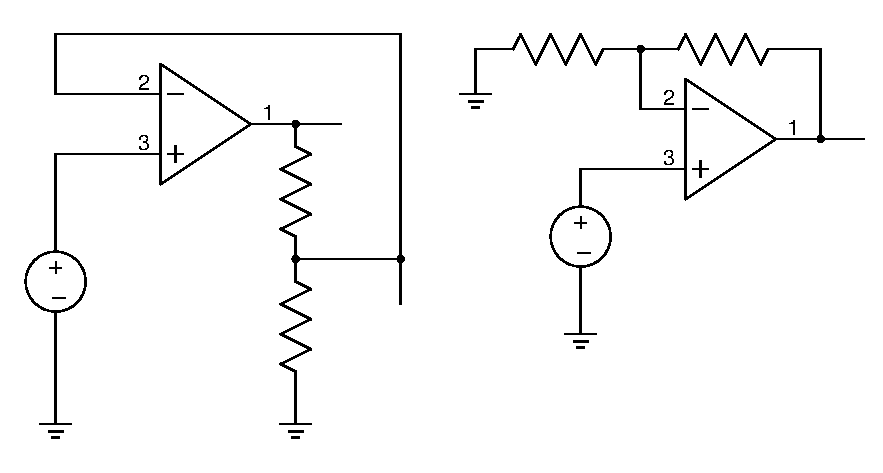
\includegraphics[scale=0.90]{voltageSeriesFeedbackNonInverting}
\caption{مثبت حسابی ایمپلیفائر ایک واپسی برقی دباو ایمپلیفائر ہے}
\label{شکل_واپسی_مثبت_واپسی_ایمپلیفائر}
\end{figure}

حسابی ایمپلیفائر کا ایک \اصطلاح {منفی داخلی سرا} جبکہ دوسرا \اصطلاح {مثبت داخلی سرا} ہے۔اس حصے میں واپسی ایمپلیفائر میں داخلی اشارہ \عددیء{V_s} کو مثبت داخلی سرے  پر مہیا کیا گیا جبکہ واپسی اشارہ \عددیء{V_f} کو منفی داخلی سرے پر مہیا کیا گیا۔جب بھی داخلی اور واپسی اشارات کو دو مختلف داخلی سروں  پر مہیا کیا جائے، انہیں سلسلہ وار جڑا تصور کریں۔چونکہ صرف برقی دباو کے اشارات کو ہی سلسلہ وار جوڑا جا سکتا ہے لہٰذا ایسی صورت میں داخلی اور واپسی اشارات کو برقی دباو اشارات تصور کریں۔مزید داخلی اشارے کو تھوِنن  شکل دیں اور واپسی اشارے کی مساوات کو برقی دباو (یعنی \عددیء{V_f})  کی صورت میں حاصل کریں۔ \عددیء{V_f} کے مساوات سے یہ بتلانا ممکن ہو گا کہ آیا \عددیء{V_o} یا \عددیء{I_o} سے واپسی اشارہ حاصل کیا گیا ہے۔ان معلومات سے ایمپلیفائر کی جماعت دریافت ہوتی ہے۔

\جزوحصہ{واپسی مزاحمت نما ایمپلیفائر}
شکل \حوالہ{شکل_واپسی_منفی_واپسی_ایمپلیفائر} الف میں منفی حسابی ایمپلیفائر دکھایا گیا ہے۔ شکل  ب میں داخلی اشارے کا نارٹن مساوی دور استعمال کیا گیا ہے۔یوں

\begin{align} \label{مساوات_واپسی_داخلی_نارٹن_اشارہ}
I_s=\frac{V_s}{R_1}
\end{align}
ہو گا۔شکل  پ کے داخلی جانب کرخوف کے قانون برائے برقی رو کی مدد سے مساوات \حوالہ{مساوات_واپسی_فرق_اشارہ} کے طرز پر
\begin{align} \label{مساوات_واپسی_واپسی_مزاحمت_نما_ایمپلیفائر_کی_جماعت_بندی}
I_i=I_s-I_f
\end{align}
لکھا جا سکتا ہے جہاں قانون اہم کی مدد سے 
\begin{align} \label{مساوات_واپسی_منفی_واپس_کار}
I_f=\frac{V_n-V_o}{R_2}=\frac{0-V_o}{R_2}=W V_o
\end{align}
%
\begin{figure}
\centering
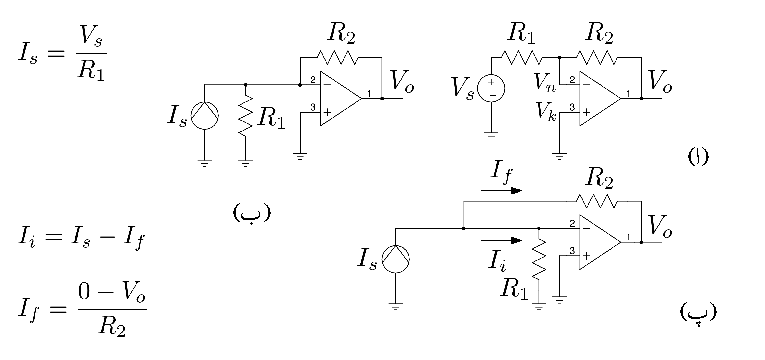
\includegraphics[scale=0.90]{voltageShuntFeedbackInverting}
\caption{منفی حسابی ایمپلیفائر ایک واپسی مزاحمت نما ایمپلیفائر ہے}
\label{شکل_واپسی_منفی_واپسی_ایمپلیفائر}
\end{figure}
%
حاصل ہوتا ہے۔مندرجہ بالا مساوات لکھتے ہوئے یاد رہے کہ حسابی ایمپلیفائر کے منفی اور مثبت داخلی سروں  پر برابر برقی دباو رہتا ہے۔چونکہ یہاں مثبت داخلی سرا برقی زمین پر ہے لہٰذا \عددیء{V_k=0} ہو گا اور اس طرح \عددیء{V_n=0} حاصل ہوتا ہے۔مساوات \حوالہ{مساوات_واپسی_منفی_واپس_کار} سے ظاہر ہے کہ واپسی اشارہ برقی رو کی صورت میں ہے اور اس کو خارجی برقی دباو سے حاصل کیا گیا ہے۔مساوات \حوالہ{مساوات_واپسی_واپسی_مزاحمت_نما_ایمپلیفائر_کی_جماعت_بندی} سے ظاہر ہے کہ داخلی جانب دو برقی رو کے اشارات کو ایک دونوں سے منفی کیا جا رہے ہے۔  یوں ان دو مساوات کو دیکھتے ہوئے ہم کہہ سکتے ہیں کہ منفی حسابی ایمپلیفائر دراصل واپسی مزاحمت نما ایمپلیفائر کی قسم ہے۔مندرجہ بالا مساوات سے
\begin{align}
W=-\frac{1}{R_2}
\end{align}
حاصل ہوتا ہے۔آپ دیکھ سکتے ہیں کہ \عددیء{R_2} ہی واپس کار ہے۔

حسابی ایمپلیفائر کی افزائش نہایت زیادہ ہوتی ہے لہٰذا منفی ایمپلیفائر مساوات  \حوالہ{مساوات_واپسی_مستحکم_افزائش_کی_شرط} پر پورا اترتا ہے اور یوں مساوات \حوالہ{مساوات_واپسی_مستحکم_افزائش} کے تحت
\begin{align}
A_{rf}=\frac{V_o}{I_s} \approx \frac{1}{W}=-R_2
\end{align}
حاصل ہوتا ہے۔مساوات \حوالہ{مساوات_واپسی_داخلی_نارٹن_اشارہ} کی مدد سے اس مساوات کو یوں لکھا جا سکتا ہے
\begin{align}
\frac{V_o}{\left(\frac{V_s}{R_1} \right)}=-R_2\\
\frac{V_o}{V_s}=-\frac{R_2}{R_1}
\end{align}
جو کہ منفی حسابی ایمپلیفائر کی جانی پہچانی مساوات ہے۔

اس حصے میں واپسی مزاحمت نما ایمپلیفائر میں داخلی اشارے  کو منفی داخلی سرے پر مہیا کیا گیا۔اسی طرح واپسی اشارے کو بھی منفی داخلی سرے پر ہی مہیا کیا گیا۔جب بھی داخلی اور واپسی اشارات کو ایک ہی داخلی سرے پر مہیا کیا جائے، انہیں متوازی جڑا تصور کریں۔ چونکہ صرف برقی رو کے اشارات کو ہی متوازی جوڑا جا سکتا ہے لہٰذا ایسی صورت میں داخلی اور واپسی اشارات کو برقی رو اشارات تصور کریں۔مزید داخلی اشارے کو نارٹن شکل دیں اور واپسی اشارے کی مساوات کو برقی رو (یعنی \عددیء{I_f}) کی صورت میں حاصل کریں۔\عددیء{I_f} کے مساوات سے یہ بتلانا ممکن ہو گا کہ آیا خارجی برقی دباو یا خارجی برقی رو سے واپسی اشارہ حاصل کیا گیا ہے۔ان معلومات سے ایمپلیفائر کی جماعت دریافت ہوتی ہے۔

\جزوحصہ{واپسی موصل نما ایمپلیفائر}
شکل \حوالہ{شکل_واپسی_ٹرانزسٹر_موصلیت_نما_ایمپلیفائر} الف میں ٹرانزسٹر کا دور دکھایا گیا ہے جس میں بوجھ \عددیء{R_L} ٹرانزسٹر کے کلکٹر پر لگایا گیا ہے۔شکل  ب میں باریک اشاراتی تجزئے کی غرض سے \عددیء{V_{CC}=0} اور \عددیء{V_{BB}=0} لئے گئے ہیں۔مزید ٹرانزسٹر کے \عددیء{V_{be}} کو \عددیء{V_i} لکھتے ہوئے
\begin{figure}
\centering
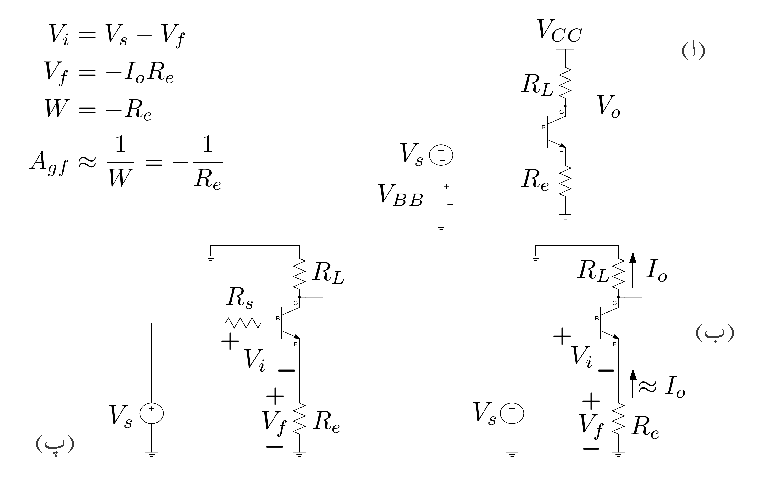
\includegraphics[scale=0.90]{npnCurrentSeriesFeedback}
\caption{ٹرانزسٹر کا واپسی موصل نما ایمپلیفائر}
\label{شکل_واپسی_ٹرانزسٹر_موصلیت_نما_ایمپلیفائر}
\end{figure}
%
\begin{align*}
V_i&=V_s-V_f \\
&=V_s-(-I_o R_e) \\
&=V_s-W I_o
\end{align*}
لکھا جا سکتا ہے۔اس کا  (\عددیء{X_i=X_s-W X_o}) کے ساتھ موازنہ کرنے سے
\begin{align}
W=-R_e 
\end{align}
حاصل ہوتا ہے۔مندرجہ بالا دو مساوات کو دیکھتے ہوئے ہم کہہ سکتے ہیں کہ یہ واپسی موصل نما ایمپلیفائر ہے اور یوں 
\begin{align}\label{مساوات_واپسی_ٹرانزسٹر_واپسی_موصلیت_نما_افزائش}
A_{gf} =\frac{I_o}{V_s}\approx \frac{1}{W}=-\frac{1}{R_e}
\end{align}
حاصل ہوتا ہے۔

حصہ \حوالہ{حصہ_واپسی_مفروضے} میں چند بنیادی مفروضے بیان کئے گئے جس کے پہلی شق کے مطابق \عددیء{W} کے قیمت پر بوجھ \عددیء{R_L} کا کوئی اثر نہیں ہو سکتا۔یوں \عددیء{W} کی قیمت یا اس کی مساوات حاصل کرتے وقت یہ خیال رہے کہ اس پر بوجھ کے مزاحمت \عددیء{R_L} کا کسی قسم کا کوئی اثر نہیں ہونا چاہئے۔اگر \عددیء{I_0=\frac{V_o}{R_L}} لکھا جائے تو \عددیء{V_f=-\frac{R_e}{R_L} V_o} لکھا جا سکتا ہے جس سے \عددیء{W=-\frac{R_e}{R_L}} حاصل ہو گا۔حاصل \عددیء{W} کی قیمت \عددیء{R_L} پر منحصر ہے جو قابل قبول نہیں۔اسی لئے اس کو غلط جواب تصور کرتے ہوئے رد کیا جاتا ہے۔

حاصل کردہ \عددیء{A_{gf}} کے استعمال سے \عددیء{\frac{V_o}{V_s}} یعنی \عددیء{A_{vf}} حاصل کرتے ہیں۔چونکہ \عددیء{V_o=I_o R_L} ہے لہٰذا
\begin{align}
A_{vf}=\frac{V_o}{V_s}=\frac{I_o R_L}{V_s}=\left(\frac{I_o}{V_s} \right ) R_L=A_{gf} R_L=-\frac{R_L}{R_e}
\end{align}
حاصل ہوتا ہے۔

اس مساوات کے مطابق \عددیء{\frac{V_o}{V_s}} کی قیمت \عددیء{R_L} سے منسلک ہے۔ اس لئے اگرچہ اسے برقی دباو کا حیطہ بڑھانے کی خاطر استعمال کیا جا سکتا ہے مگر یہ ہرگز برقی دباو ایمپلیفائر نہیں ہے اور جب بھی بوجھ \عددیء{R_L} تبدیل کی جائے اس ایمپلیفائر کی \عددیء{\frac{V_o}{V_s}} کی شرح تبدیل ہو جائے گی۔اس کے برعکس مساوات \حوالہ{مساوات_واپسی_ٹرانزسٹر_واپسی_موصلیت_نما_افزائش} کے تحت \عددیء{\frac{I_o}{V_s}} کے قیمت پر \عددیء{R_L} کا کوئی اثر نہیں لہٰذا اس ایمپلیفائر کو واپسی موصل نما ایمپلیفائر تصور کیا جائے گا۔

شکل  پ میں \عددیء{R_s} بھی شامل کیا گیا ہے۔یہاں \عددیء{R_s} کو ایمپلیفائر کا اندرونی حصہ تصور کرتے ہوئے \عددیء{V_i=V_s-V_f} لکھا جا سکتا ہے۔یوں مندرجہ بالا تمام تبصرہ اس شکل کے لئے بھی درست ہے۔

ٹرانزسٹر کے \عددیء{B} اور \عددیء{E} کو دو علیحدہ داخلی سرے تصور کیا جا سکتا ہے \حاشیہد{ایسا کرتے ہوئے \عددیء{B} کو منفی جبکہ \عددیء{E} کو مثبت داخلی سرا تصور کریں}۔یوں اس حصے میں واپسی موصل نما ایمپلیفائر میں داخلی اشارے  کو \عددیء{B} پر مہیا کیا گیا جبکہ واپسی اشارے کو \عددیء{E} پر مہیا کیا گیا۔جب بھی داخلی اور واپسی اشارات کو دو مختلف داخلی سروں پر مہیا کیا جائے، انہیں سلسلہ وار جڑا تصور کریں۔چونکہ صرف برقی دباو اشارات ہی سلسلہ وار جوڑے جا سکتے ہیں لہٰذا ایسی صورت میں داخلی اور واپسی اشارات کو برقی دباو  اشارات تصور کریں۔ مزید داخلی اشارے کو تھوِنن  شکل دیں جبکہ واپسی اشارے کی مساوات کو برقی دباو (یعنی \عددیء{V_f}) کی صورت میں حاصل کریں۔

واپسی اشارے کی مساوات سے یہ بتلانا ممکن ہو گا کہ آیا \عددیء{V_o} یا \عددیء{I_o} سے واپسی اشارہ حاصل کیا گیا ہے۔ان معلومات سے ایمپلیفائر کی جماعت دریافت ہوتی ہے۔اس صورت میں \عددیء{B} اور \عددیء{E} کے مابین برقی دباو کو \عددیء{V_i} لکھا جائے گا۔



\جزوحصہ{واپسی برقی رو ایمپلیفائر}
شکل \حوالہ{شکل_واپسی_ٹرانزسٹر_برقی_رو_ایمپلیفائر} الف میں ٹرانزسٹر کا دور دکھایا گیا ہے جس میں بوجھ \عددیء{R_L} ٹرانزسٹر \عددیء{Q_2} کے  کلکٹر  پر لگایا گیا ہے۔شکل  ب میں باریک اشاراتی تجزئے کی غرض سے کپیسٹر کو قصر دور اور \عددیء{V_{CC}=V_{BB}=0} لیا گیا ہے۔مزید داخلی اشارے کا نارٹن مساوی دور استعمال کیا گیا ہے اور \عددیء{R_s} کو ایمپلیفائر کا حصہ تصور کیا گیا ہے۔یوں کرخوف کے قانون برائے برقی رو کی مدد سے ہم لکھ سکتے ہیں۔
\begin{figure}
\centering
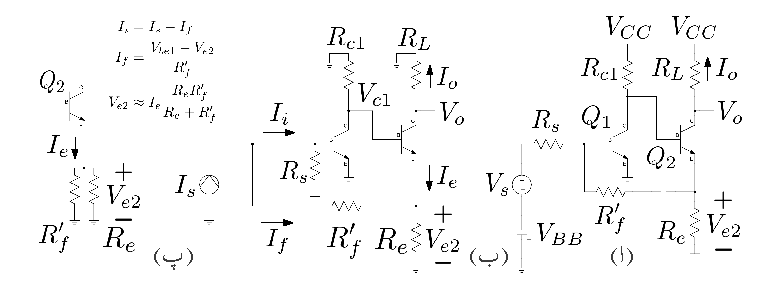
\includegraphics[scale=0.90]{npnCurrentShuntFeedback}
\caption{ٹرانزسٹر کا واپسی برقی رو ایمپلیفائر}
\label{شکل_واپسی_ٹرانزسٹر_برقی_رو_ایمپلیفائر}
\end{figure}
%
\begin{align*} \label{مساوات_واپسی_ٹرانزسٹر_برقی_رو_ایمپلیفائر_واپسی_مساوات}
I_i=I_s-I_f
\end{align*}
جہاں
\begin{align*}
I_f=\frac{V_{be1}-V_{e2}}{R_f'}
\end{align*}
کے برابر ہے۔کامل واپسی ادوار میں واپسی اشارے کی مساوات \عددیء{X_f=WX_o} ہوتی ہے۔ٹرانزسٹر واپسی ادوار کامل ادوار نہیں ہوتے۔مندرجہ بالا مساوات میں \عددیء{\tfrac{V_{be1}}{R_f'}}  کا واپسی اشارہ پیدا کرنے میں کوئی کردار نہیں چونکہ \عددیء{V_{be1}} داخلی جانب کا متغیرہ ہے نا کہ خارجی جانب کا۔یوں مندرجہ بالا مساوات میں \عددیء{\tfrac{V_{be1}}{R_f'}} غیر ضروری جزو ہے۔یہ جزو اس لئے پایا گیا ہے کہ ٹرانزسٹر ادوار کامل واپسی ادوار نہیں ہوتے۔اس غیر ضروری جزو کو نظر انداز کرتے ہوئے 
\begin{align*}
I_f \approx -\frac{V_{e2}}{R_f'}
\end{align*}
حاصل ہوتا ہے۔اسی طرح جیسے شکل  پ میں دکھایا گیا ہے، \عددیء{V_{be1}} کو نظر انداز  کرتے ہوئے (یعنی \عددیء{V_{be1}=0} لیتے ہوئے) \عددیء{R_e} اور \عددیء{R_f'} کو متوازی تصور کیا جا سکتا ہے اور یوں
\begin{align*}
V_{e2} &\approx I_e \left (\frac{R_e R_f'}{R_e+R_f'}\right )\\
&=-I_o \left ( \frac{R_e R_f'}{R_e+R_f'}\right )
\end{align*}
حاصل ہوتا ہے جہاں \عددیء{I_e \approx -I_o} کے برابر لیا گیا ہے۔اس طرح
\begin{align*}
I_f \approx -\frac{V_{e2}}{R_f'}=\left(\frac{R_e}{R_e+R_f'} \right) I_o
\end{align*}
لکھا جا سکتا ہے  جس سے
\begin{align*}
W =\frac{R_e}{R_e+R_f'}
\end{align*}
حاصل ہوتا ہے۔

آپ دیکھ سکتے ہیں کہ یہ واپسی برقی رو ایمپلیفائر ہے اور یوں
\begin{align}
A_{if} \approx \frac{1}{W}=1+\frac{R_f'}{R_e}
\end{align}
لکھا جا سکتا ہے۔

اس ایمپلیفائر کا \عددیء{\frac{V_o}{V_s}} یوں حاصل کیا جا سکتا ہے۔
\begin{gather}
\begin{aligned}
A_{vf}&=\frac{V_o}{V_s}=\frac{I_o R_L}{I_s R_s}=\left (\frac{I_o}{I_s} \right) \left (\frac{R_L}{R_s} \right) \\
&=A_{if} \left(\frac{R_L}{R_s} \right)=\left( 1+\frac{R_f'}{R_e}\right) \left(\frac{R_L}{R_s} \right)
\end{aligned}
\end{gather}
%
اس حصے میں  داخلی اور واپسی دونوں اشارات کو ٹرانزسٹر کے \عددیء{B} پر مہیا کیا گیا۔ جب بھی ان  دو اشارات کو ایک ہی داخلی سرے پر مہیا کیا جائے، انہیں متوازی جڑا تصور کریں۔چونکہ صرف برقی رو اشارات ہی متوازی جوڑے جا سکتے ہیں لہٰذا ایسی صورت میں داخلی اور واپسی اشارات کو برقی رو اشارات تصور کریں۔ مزید داخلی اشارے کو نارٹن شکل دیں جبکہ واپسی اشارے کی مساوات کو برقی رو (یعنی \عددیء{I_f}) کی صورت میں حاصل کریں۔واپسی اشارے کی مساوات سے یہ بتلانا ممکن ہو گا کہ آیا \عددیء{V_o} یا \عددیء{I_o} سے واپسی اشارہ حاصل کیا گیا ہے۔ان معلومات سے ایمپلیفائر کی جماعت دریافت ہوتی ہے۔ 

 جس داخلی سرے پر داخلی اشارہ جڑا ہو اگر اسی نقطے پر مزاحمت (یا کپیسٹر وغیرہ) کا ایک سرا جڑا ہو جبکہ اس مزاحمت (یا کپیسٹر) کا دوسرا سرا ایمپلیفائر کے خارجی جانب جڑا ہو تو ایسی صورت میں داخلی اور واپسی اشارات متوازی جڑے ہوتے ہیں۔
%-----
\جزوحصہ{واپسی مزاحمت نما ایمپلیفائر}
شکل \حوالہ{شکل_واپسی_ٹرانزسٹر_مزاحمت_نما_ایمپلیفائر} الف میں ٹرانزسٹر کا دور دکھایا گیا ہے جس میں بوجھ \عددیء{R_L} ٹرانزسٹر کے \عددیء{E} پر لگایا گیا ہے۔شکل  ب میں باریک اشاراتی تجزئے کی غرض سے کپیسٹر کو قصر دور کیا گیا ہے اور  \عددیء{V_{CC}=V_{BB}=0} لیا گیا ہے۔مزید داخلی اشارے کا نارٹن مساوی دور استعمال کیا گیا ہے اور \عددیء{R_s} کو ایمپلیفائر کا حصہ تصور کیا گیا ہے۔یوں ہم لکھ سکتے ہیں
\begin{align} \label{مساوات_واپسی_مزاحمت_نما_واپسی_رو_اشارہ}
I_i&=I_s-I_f
\end{align}
جہاں \عددیء{I_s=\frac{V_s}{R_s}} اور
\begin{align*}
I_f&=\frac{V_{be}-V_o}{R_f} \\
&=\frac{V_{be}}{R_f}-\frac{V_o}{R_f}
\end{align*}
کے برابر ہے۔اس مساوات میں \عددیء{\frac{V_{be}}{R_f}} کا واپسی اشارہ پیدا کرنے میں کوئی کردار نہیں البتہ \عددیء{-\frac{V_o}{R_f}} خارجی برقی دباو پر منحصر واپسی اشارہ ہے یوں مساوات کے پہلے جزو کو نظر انداز کرتے ہوئے ہم لکھ سکتے ہیں
\begin{align*}
I_f & \approx -\frac{V_o}{R_f} \\
&=W V_o \\
W&=-\frac{1}{R_f}
\end{align*}
اور یوں مساوات \حوالہ{مساوات_واپسی_مزاحمت_نما_واپسی_رو_اشارہ} کو ہم لکھ سکتے ہیں
\begin{align*}
I_i &\approx I_s-\left(-\frac{V_o}{R_f} \right) \\
&=I_s-W V_o
\end{align*}
جس سے ہم کہہ سکتے ہیں کہ یہ مزاحمت نما واپسی ایمپلیفائر ہے اور یوں
\begin{align}
A_{rf} \approx \frac{1}{W}=-R_f
\end{align}
ہو گا۔

اسی ایمپلیفائر کا \عددیء{\frac{V_o}{V_s}} یعنی \عددیء{A_{vf}} یوں حاصل کیا جا سکتا ہے۔
\begin{align}
A_{vf}=\frac{V_o}{V_s}=\frac{V_o}{I_s R_s}=\left (\frac{V_o}{I_s} \right ) \frac{1}{R_s}=\frac{A_{rf}}{R_s}=-\frac{R_f}{R_s}
\end{align}
اسی طرح \عددیء{\frac{I_o}{I_s}} یوں حاصل ہو گا
\begin{align}
A_{if}=\frac{I_o}{I_s}=\frac{\frac{V_o}{R_L}}{I_s}=\left (\frac{V_o}{I_s} \right) \frac{1}{R_L}=\frac{A_{rf}}{R_L}=-\frac{R_f}{R_L}
\end{align}
اور \عددیء{\frac{I_o}{V_s}} کو یوں
\begin{align}
A_{gf}=\frac{I_o}{V_s}=\frac{\frac{V_o}{R_L}}{I_s R_s}=\left (\frac{V_o}{I_s} \right) \frac{R_s}{R_L}=A_{rf}\frac{R_s}{R_L}=-\frac{R_f R_s}{R_L}
\end{align}
%
\begin{figure}
\centering
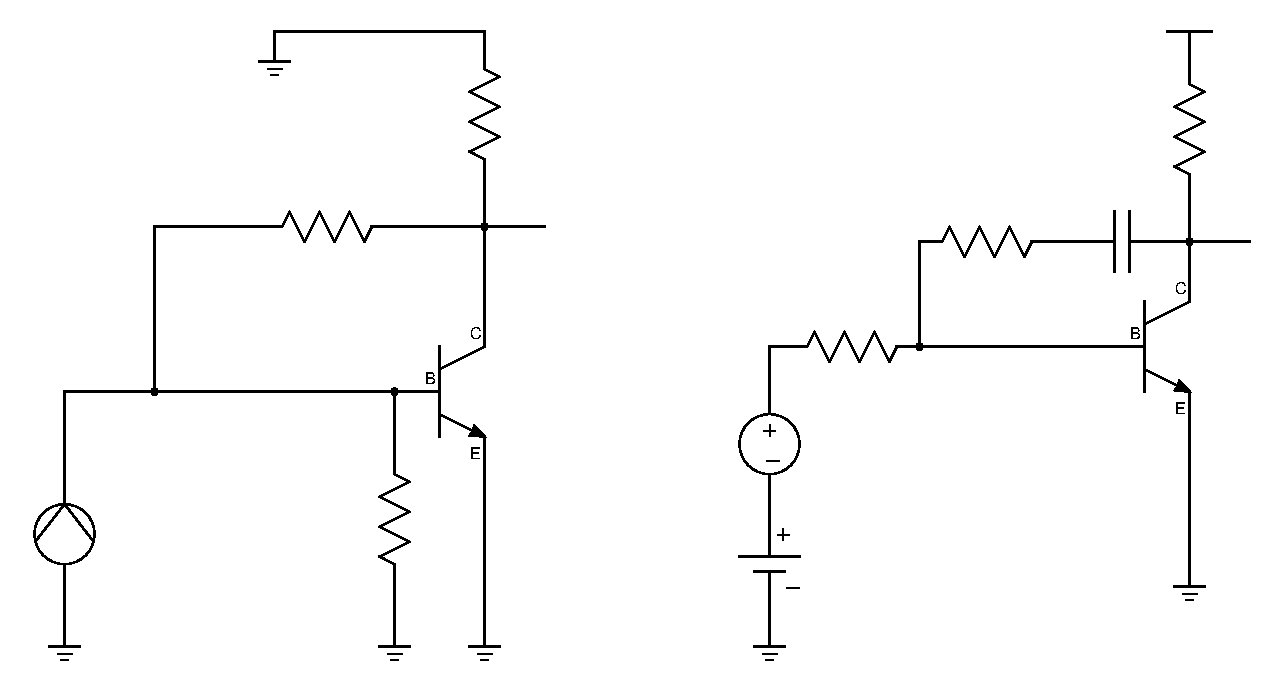
\includegraphics[scale=0.90]{npnVoltageShuntFeedback}
\caption{ٹرانزسٹر کا واپسی مزاحمت نما ایمپلیفائر}
\label{شکل_واپسی_ٹرانزسٹر_مزاحمت_نما_ایمپلیفائر}
\end{figure}
شکل \حوالہ{شکل_واپسی_ٹرانزسٹر_واپسی_نقطہ} الف، ب اور پ میں شکل \حوالہ{شکل_واپسی_ٹرانزسٹر_مزاحمت_نما_ایمپلیفائر}، شکل \حوالہ{شکل_واپسی_ٹرانزسٹر_برقی_رو_ایمپلیفائر} اور شکل \حوالہ{شکل_واپسی_ٹرانزسٹر_موصلیت_نما_ایمپلیفائر} دوبارہ دکھائے گئے ہیں۔شکل  الف پر غور کریں۔اس میں خارجی دائرے کی نشاندہی کی گئی ہے۔خارجی جانب برقی دباو \عددیء{V_o} اور برقی رو \عددیء{I_o} کی بھی نشاندہی کی گئی ہے۔ٹرانزسٹر کے \عددیء{C} جہاں سے \عددیء{V_o} یا (اور) \عددیء{I_o} حاصل کیا گیا ہے کو خارجی نقطہ قرار دیا گیا ہے۔بوجھ \عددیء{R_L} کو خارجی نقطے  پر جوڑا جاتا ہے۔اسی طرح واپسی نقطے  کی بھی نشاندہی کی گئی ہے۔یہ وہ نقطہ ہے جہاں سے واپس کار اشارہ حاصل کرتا ہے۔یہاں \عددیء{R_f} بطور واپس کار کردار ادا کر رہا ہے۔اس شکل میں واپسی نقطہ اور خارجی نقطہ دونوں ایک ہی جوڑ پر پائے جاتے ہیں۔ایسی صورت جہاں خارجی نقطہ  اور واپسی نقطہ ایک ہی جوڑ پر پائے جائیں میں واپس کار خارجی برقی دباو \عددیء{V_o} سے واپسی اشارہ حاصل کرتا ہے۔

شکل \حوالہ{شکل_واپسی_ٹرانزسٹر_واپسی_نقطہ} ب میں خارجی نقطہ اور واپسی نقطہ دو علیحدہ علیحدہ جوڑ پر پائے جاتے ہیں۔یوں واپسی اشارے کو اس جوڑ سے حاصل نہیں کیا گیا جہاں سے \عددیء{V_o} یا \عددیء{I_o} حاصل کیا گیا ہے۔البتہ واپسی اشارے کو خارجی دائرے سے حاصل کیا گیا ہے۔خارجی دائرہ وہ دائرہ ہے جس میں خارجی برقی رو \عددیء{I_o} کا بہاو ہوتا ہے۔ایسی صورت جہاں خارجی نقطہ  اور واپسی نقطہ دو علیحدہ علیحدہ جوڑ پر پائے جائیں میں واپس کار خارجی برقی رو \عددیء{I_o} سے واپسی اشارہ حاصل کرتا ہے۔

شکل \حوالہ{شکل_واپسی_ٹرانزسٹر_واپسی_نقطہ} پ میں مزاحمت \عددیء{R_e} کو \عددیء{R_f} لکھا گیا ہے۔یہاں بھی خارجی اور واپسی نقطے دو علیحدہ علیحدہ جوڑ پر پائے جاتے ہیں لہٰذا یہاں بھی واپس کار خارجی برقی رو \عددیء{I_o} سے واپسی اشارہ حاصل کرتا ہے۔
\begin{figure}
\centering
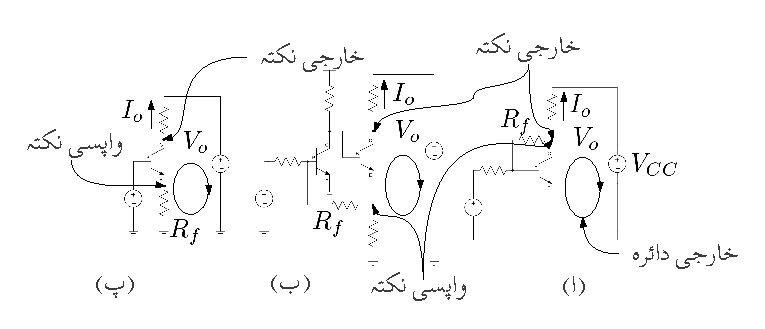
\includegraphics[scale=0.90]{npnFeedbackOutputPoint}
\caption{واپسی نقطہ}
\label{شکل_واپسی_ٹرانزسٹر_واپسی_نقطہ}
\end{figure}


\حصہ{واپسی ایمپلیفائر کا تفصیلی تجزیہ} \label{حصہ_واپسی_تفصیلی_تجزیہ}
اب تک مساوات \حوالہ{مساوات_واپسی_مستحکم_افزائش_کی_شرط} پر پورا اترتے واپسی ایمپلیفائروں پر غور کیا گیا۔اس حصے میں ان واپسی ایمپلیفائر پر غور کیا جائے گا جو اس مساوات پر پورا نہیں اترتے۔ایسا کرتے وقت ایمپلیفائر کو دو حصوں یعنی بنیادی ایمپلیفائر \عددیء{A} اور واپس کار \عددیء{W}  میں تقسیم کیا جاتا ہے۔واپسی ایمپلیفائر میں واپسی اشارے کو صفر کرتے ہوئے مگر واپس کار کے بوجھ کو شامل کرتے ہوئے بنیادی ایمپلیفائر حاصل کیا جاتا ہے۔مندرجہ ذیل اقدام کی مدد سے ایسا کیا جاتا ہے۔

بنیادی ایمپلیفائر کا داخلی حصہ حاصل کرنے کی خاطر خارجی اشارہ \عددیء{X_o} کی قیمت کو صفر کر دیا جاتا ہے۔یعنی
\begin{itemize}
\item
اگر خارجی برقی دباو \عددیء{V_o} سے واپسی اشارہ حاصل کیا گیا ہو (یعنی \عددیء{X_f=W X_o}) تو خارجی برقی دباو کو قصر دور کر کے \عددیء{V_o=0} کر دیا جاتا ہے جس سے \عددیء{X_f} بھی صفر ہو جاتا ہے۔
\item
اس کے برعکس اگر واپسی اشارے کو \عددیء{I_o} سے حاصل کیا گیا ہو تب خارجی دائرے کو کھلے سرے کر دیا جاتا ہے۔ یوں \عددیء{I_o=0} ہو جاتا ہے جس سے \عددیء{X_f} بھی صفر ہو جاتا ہے۔
\end{itemize} 


بنیادی ایمپلیفائر کا خارجی حصہ حاصل کرنے کی خاطر کل داخلی اشارہ \عددیء{X_i} کی قیمت صفر کر دیا جاتا ہے۔یعنی
\begin{itemize}
\item
اگر داخلی اور واپسی اشارات متوازی جڑے ہوں تب یہ دونوں برقی رو اشارات ہوں گے۔انہیں قصر دور کرنے سے \عددیء{I_i=0} کیا جاتا ہے۔
\item
اس کے برعکس اگر داخلی اور واپسی اشارات سلسلہ وار جڑے ہوں تب یہ دونوں برقی دباو اشارات ہوں گے۔داخلی دائرے کو کھلے سرے کرنے سے \عددیء{V_i=0} کیا جاتا ہے۔
\end{itemize} 
اس ترکیب سے واپسی اشارہ کے اثرات کو ختم کر دیا جاتا ہے جبکہ بنیادی ایمپلیفائر پر واپس کار کے بوجھ کے اثرات برقرار رہنے دئے جاتے ہیں۔اس ترکیب کو استعمال کرتے ہوئے واپسی ایمپلیفائر حل کرنے کے مکمل اقدام مندرجہ ذیل ہیں۔

\begin{itemize}
\item
پہلے یہ فیصلہ کریں کہ \عددیء{X_f} برقی دباو یا برقی رو کا اشارہ ہے۔اگر \عددیء{X_f} داخلی اشارہ \عددیء{X_s} کے ساتھ سلسلہ وار جڑا ہو تو \عددیء{X_f} برقی دباو اشارہ ہو گا اور اگر یہ \عددیء{X_s} کے ساتھ متوازی جڑا ہو تب \عددیء{X_f} برقی رو اشارہ ہو گا۔اسی طرح فیصلہ کریں کہ \عددیء{X_o} برقی دباو یا برقی رو اشارہ ہے۔اگر \عددیء{X_f} کو \عددیء{X_o} جوڑ سے حاصل کیا گیا ہو تب \عددیء{X_o} برقی دباو اشارہ ہو گا اور اگر \عددیء{X_f} خارجی دائرہ سے حاصل کیا گیا ہو تب \عددیء{X_o} برقی رو اشارہ ہو گا۔
\item
واپسی ایمپلیفائر کی جماعت دریافت کریں۔اگر \عددیء{X_s} اور \عددیء{X_f} سلسلہ وار جڑے ہوں تب \عددیء{X_f} برقی دباو اشارہ یعنی \عددیء{V_f} ہو گا اور اگر یہ دونوں متوازی جڑے ہوں تب \عددیء{X_f} برقی رو اشارہ یعنی \عددیء{I_f} ہو گا۔اسی طرح اگر واپسی اشارے کو خارجی نقطے  سے حاصل کیا گیا ہو تب واپسی اشارے کو \عددیء{V_o} سے حاصل گیا ہو گا اور خارجی اشارے کو \عددیء{V_o} تصور کیا جائے گا۔اس کے برعکس اگر واپسی اشارے کو خارجی دائرے سے حاصل کیا گیا ہو تب خارجی اشارہ \عددیء{I_o} تصور کیا جائے گا۔
\item 
واپسی اشارے کا اثر ختم کرتے ہوئے مگر واپس کار کے بوجھ کے اثر کو برقرار رکھتے ہوئے مندرجہ بالا قوانین کی مدد سے بنیادی ایمپلیفائر کا دور حاصل کریں۔اگر \عددیء{X_f} اور \عددیء{X_s} سلسلہ وار جڑے ہوں تب داخلی اشارہ \عددیء{X_s} کا تھوِنن  مساوی دور استعمال کریں۔اس کے برعکس اگر \عددیء{X_f} اور \عددیء{X_s} متوازی جڑے ہوں تب داخلی اشارہ \عددیء{X_s} کا نارٹن مساوی دور استعمال کریں۔
\item
بنیادی ایمپلیفائر میں ٹرانزسٹر کا ریاضی نمونہاستعمال کرتے ہوئے اس کا باریک اشاراتی مساوی دور حاصل کریں اور اس میں \عددیء{X_f} اور \عددیء{X_o} کی نشاندہی کریں۔
\item
واپسی اشارے \عددیء{X_f=W X_o} کی مساوات حاصل کریں جس سے \عددیء{W} کی قیمت حاصل ہو گی۔
\item
کرخوف کے قوانین استعمال کرتے ہوئے بنیادی ایمپلیفائر سے افزائش \عددیء{A}، داخلی مزاحمت \عددیء{R_i} اور خارجی مزاحمت \عددیء{R_o} حاصل کریں۔
\item
مندرجہ بالا حاصل کردہ معلومات سے \عددیء{A_f}، \عددیء{R_{if}'} اور \عددیء{R_{of}} حاصل کریں۔
\end{itemize}

آئیں اس ترکیب کو استعمال کرتے ہوئے واپسی ایمپلیفائر حل کریں۔

\حصہ{واپسی برقی دباو ایمپلیفائر}
شکل \حوالہ{شکل_واپسی_بنیادی_ایمپلیفائر_کا_حصول} الف میں واپسی برقی دباو ایمپلیفائر دکھایا گیا ہے۔نقطہ مائل حاصل کرنے کی خاطر \عددیء{V_s} کے ساتھ \عددیء{V_{BB}} سلسلہ وار تصور کریں جس کو شکل میں نہیں دکھایا گیا تا کہ اصل مضمون پر توجہ رکھنی آسان ہو۔اس دور کو قدم با قدم حل کرتے ہیں۔
\begin{figure}
\centering
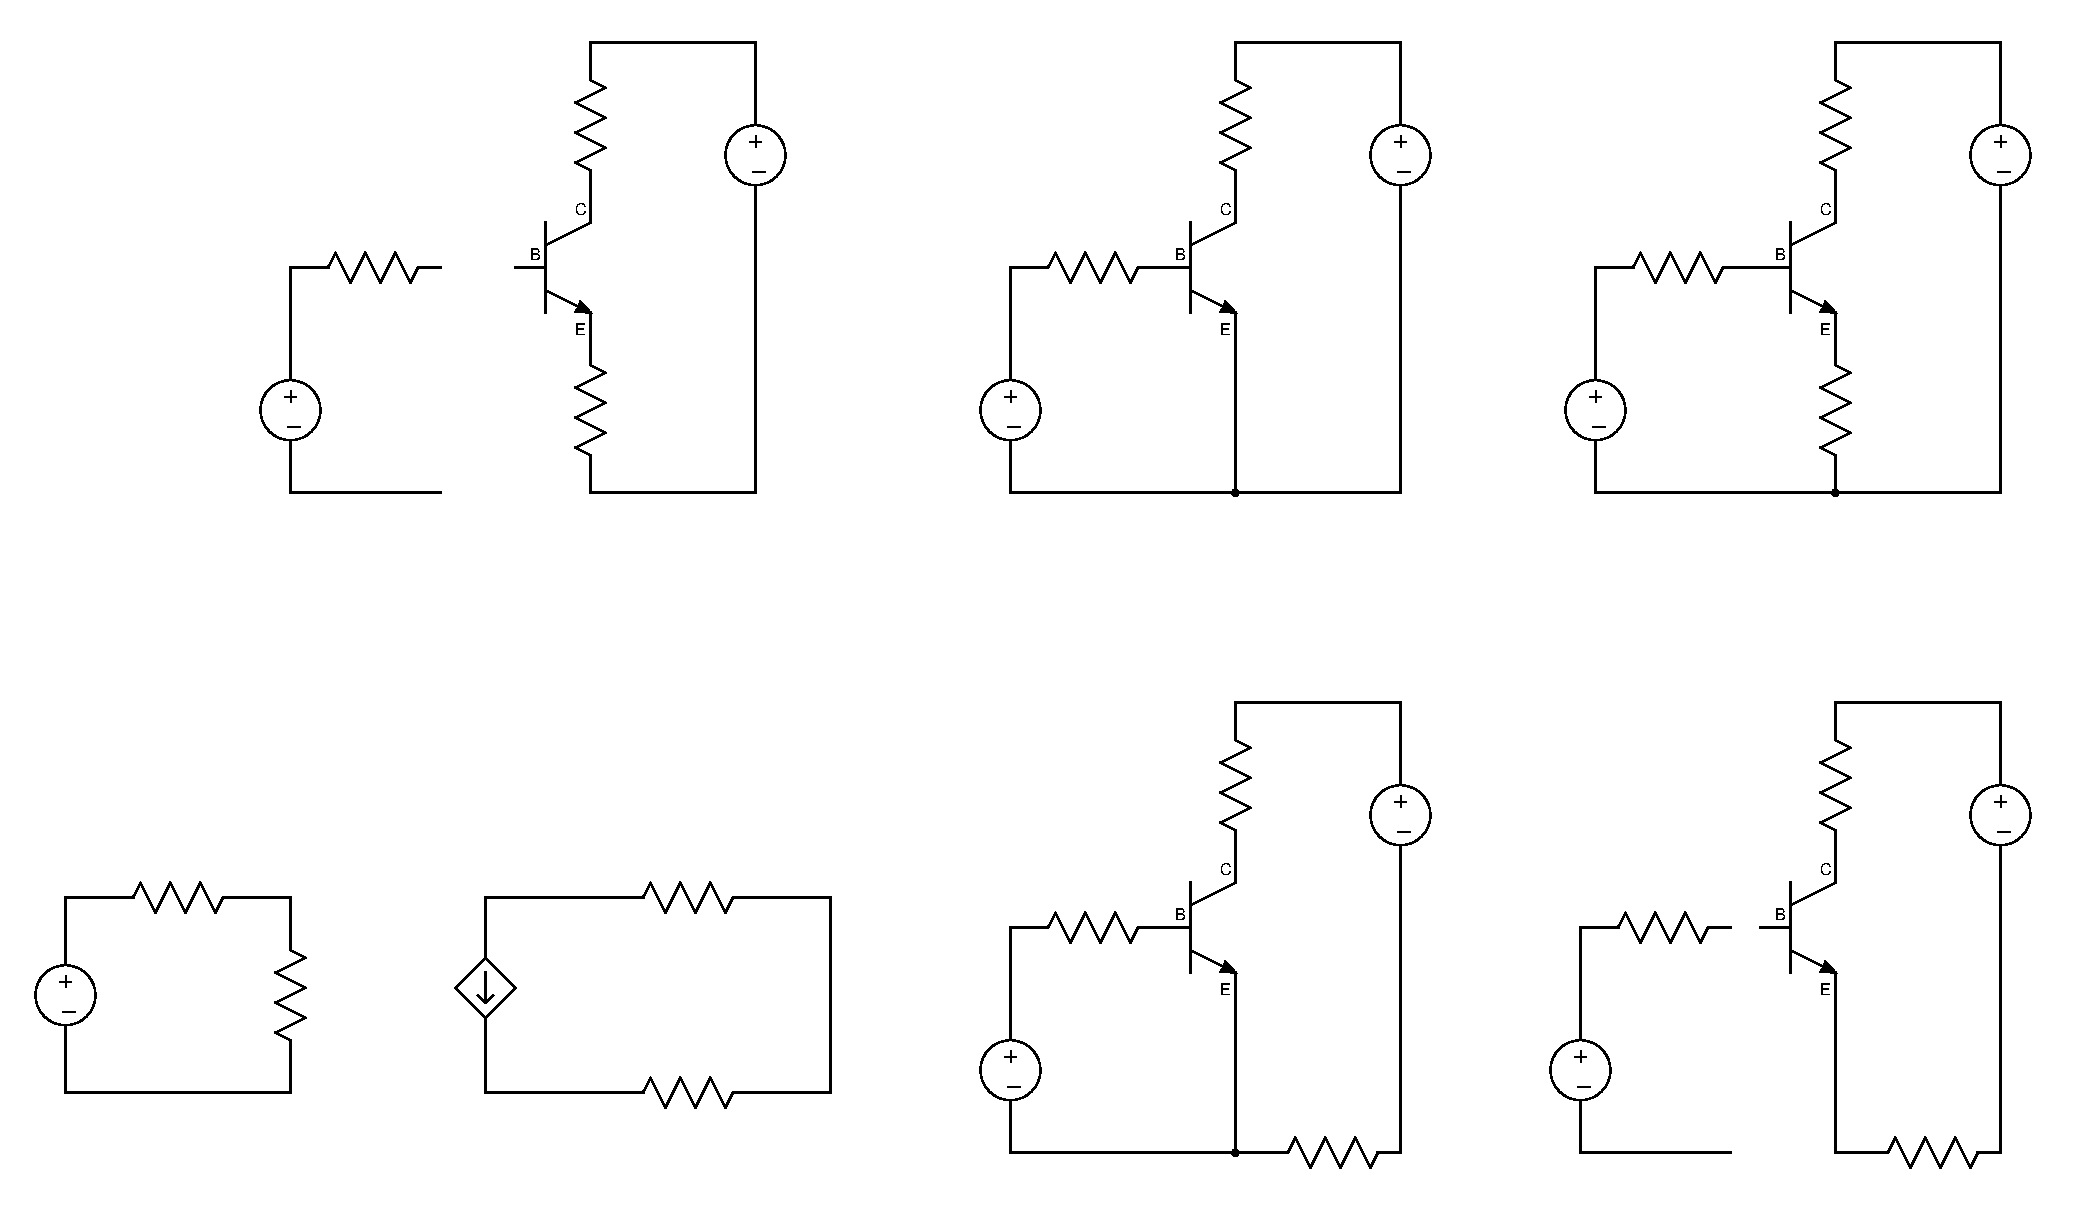
\includegraphics[scale=0.90]{npnVoltageSeriesEmitterFollowerDetailed}
\caption{بنیادی ایمپلیفائر کا حصول}
\label{شکل_واپسی_بنیادی_ایمپلیفائر_کا_حصول}
\end{figure}

پہلے قدم پر اس کی جماعت جاننا ضروری ہے۔اس دور پر تفصیلی بحث ہو چکی ہے۔یہ واپسی برقی دباو ایمپلیفائر ہے۔

چونکہ \عددیء{V_o} سے واپسی اشارہ حاصل کیا گیا ہے لہٰذا، بنیادی ایمپلیفائر کا داخلی مساوی دور حاصل کرنے کی خاطر \عددیء{V_o} کو قصر دور کرتے ہیں۔ایسا شکل  ب میں دکھایا گیا ہے جہاں صرف داخلی دائرے پر نظر رکھتے ہوئے ہم لکھ سکتے ہیں
\begin{align} \label{مساوات_واپسی_برقی_دباو_داخلی_مساوی}
V_s = I_s R_s +V_{be}
\end{align}
چونکہ داخلی جانب \عددیء{V_s} اور \عددیء{V_f} سلسلہ وار جڑے ہیں لہٰذا بنیادی ایمپلیفائر کا خارجی مساوی دور حاصل کرنے کی خاطر داخلی دائرے کو کھلے سرے کر دیا جاتا ہے۔ایسا شکل  پ میں دکھایا گیا ہے۔اس شکل میں صرف خارجی دائرے پر نظر رکھتے ہوئے ہم لکھ سکتے ہیں
\begin{align} \label{مساوات_واپسی_برقی_دباو_خارجی_مساوی}
V_{CC} &= I_c R_c+V_{ce}+I_c R_L 
\end{align}
شکل  پ کو قدر مختلف طرز پر شکل  ت میں دوبارہ دکھایا گیا ہے جہاں \عددیء{V_o} اور \عددیء{V_f} کی نشاندہی بھی کی گئی ہے۔آپ تسلی کر لیں کہ اس شکل کے 
خارجی دائرے کی مساوات  بھی مندرجہ بالا مساوات ہی ہے۔شکل  ب کے داخلی مساوی دور اور شکل  ت کے خارجی مساوی دور کو ملا کر شکل  ٹ حاصل ہوتا ہے۔شکل  ٹ کے داخلی اور خارجی مساوات یوں حاصل ہوں گے۔
\begin{align}
V_s &= I_s R_s +V_{be}\\
V_{CC} &= I_c R_c+V_{ce}+I_c R_L
\end{align}
یہ بالکل مساوات \حوالہ{مساوات_واپسی_برقی_دباو_داخلی_مساوی} اور مساوات \حوالہ{مساوات_واپسی_برقی_دباو_خارجی_مساوی} ہی ہیں۔

شکل  ث میں ٹرانزسٹر کا پائے ریاضی نمونہاستعمال کرتے ہوئے شکل  ٹ کا باریک اشاراتی دور حاصل کیا گیا ہے۔اس سے
\begin{align} \label{مساوات_واپسی_ٹرانزسٹر_تابع_مخارج_افزائش}
A_V=\frac{V_o}{V_s}=\frac{V_o}{I_c} \times \frac{I_c}{V_{be}} \times \frac{V_{be}}{V_s}=\frac{R_L g_m r_{be}}{R_s+r_{be}}=\frac{\beta R_L}{R_s+r_{be}}
\end{align}
حاصل ہوتا ہے جہاں مساوات \حوالہ{مساوات_ٹرانزسٹر_داخلی_مزاحمت_بالمقابل_موصلیت_نما} کے تحت \عددیء{g_m r_{be}=\beta} کے برابر ہے۔شکل  ٹ سے  \عددیء{V_f=V_o}  لہٰذا \عددیء{W =1} حاصل ہوتا ہے۔اس طرح
\begin{align}
M=1+W A_V=1+\frac{\beta R_L}{R_s+r_{be}}=\frac{R_s+r_{be}+\beta R_L}{R_s+r_{be}}
\end{align}
ہے۔

بنیادی ایمپلیفائر کا داخلی مزاحمت
\begin{align}
R_i'=R_s+r_{be}
\end{align}
کے برابر ہے اور یوں
\begin{align}
R_{if}'=M R_i' =\left (R_s+r_{be} \right) \times \frac{R_s+r_{be}+\beta R_L}{R_s+r_{be}}=R_s+r_{be}+\beta R_L
\end{align}
حاصل ہوتا ہے۔

مساوات \حوالہ{مساوات_واپسی_لامحدود_مزاحمت_پر_افزائش_برقی_دباو_ب} کے تحت \عددیء{A_v'=\left . A_V \right|_{R_L \to \infty}} ہے۔یوں مساوات \حوالہ{مساوات_واپسی_ٹرانزسٹر_تابع_مخارج_افزائش} میں \عددیء{R_L \to \infty} کے استعمال سے \عددیء{A_v'=\infty} حاصل ہوتا ہے۔خارجی مزاحمت \عددیء{R_o} حاصل کرتے وقت بوجھ \عددیء{R_L} کو ایمپلیفائر کا حصہ تصور نہیں کیا جاتا اور یوں شکل  ٹ سے \عددیء{R_o = \infty} حاصل ہوتا ہے جس سے
\begin{align*} \label{مساوات_واپسی_تابع_مخارج_خارجی_مزاحمت_مسئلہ}
R_{of}=\frac{R_o}{1+W A_v'} =\frac{\infty}{\infty}
\end{align*}
حاصل ہوتا ہے جس کا کوئی مطلب نہیں۔

مساوات \حوالہ{مساوات_واپسی_تابع_مخارج_خارجی_مزاحمت_مسئلہ} سے خارجی مزاحمت حاصل کرنا ممکن نہیں۔\عددیء{R_of} حاصل کرنے کی خاطر  دور سے پہلے \عددیء{R_{of}'} حاصل کریں اور پھر مساوات \حوالہ{مساوات_واپسی_لامحدود_بار_مزاحمت__پر_مزاحمت} کی مدد سے  \عددیء{R_o} حاصل کریں۔

\عددیء{R_L} کی شمولیت سے \عددیء{R_{o}'} کی قیمت \عددیء{R_L} کے برابر ہے۔اس طرح
\begin{align}
R_{of}'=\frac{R_o'}{M}=\frac{R_L(R_s+r_{be})}{R_s+r_{be}+\beta R_L}
\end{align}
اور
\begin{align}
R_{of}=\left. R_{of}'\right|_{R_L \to \infty} =\frac{R_s+r_{be}}{\beta}
\end{align}
حاصل ہوتا ہے۔
%
\حصہ{واپسی برقی دباو زنجیری ایمپلیفائر}
شکل \حوالہ{شکل_واپسی_دو_درجہ_واپسی_برقی_دباو_ایمپلیفائر} میں دو کڑی زنجیری ایمپلیفائر دکھایا گیا  ہے۔درکار تعدد پر تمام کپیسٹروں کو قصر دور تصور کریں۔
\begin{figure}
\centering
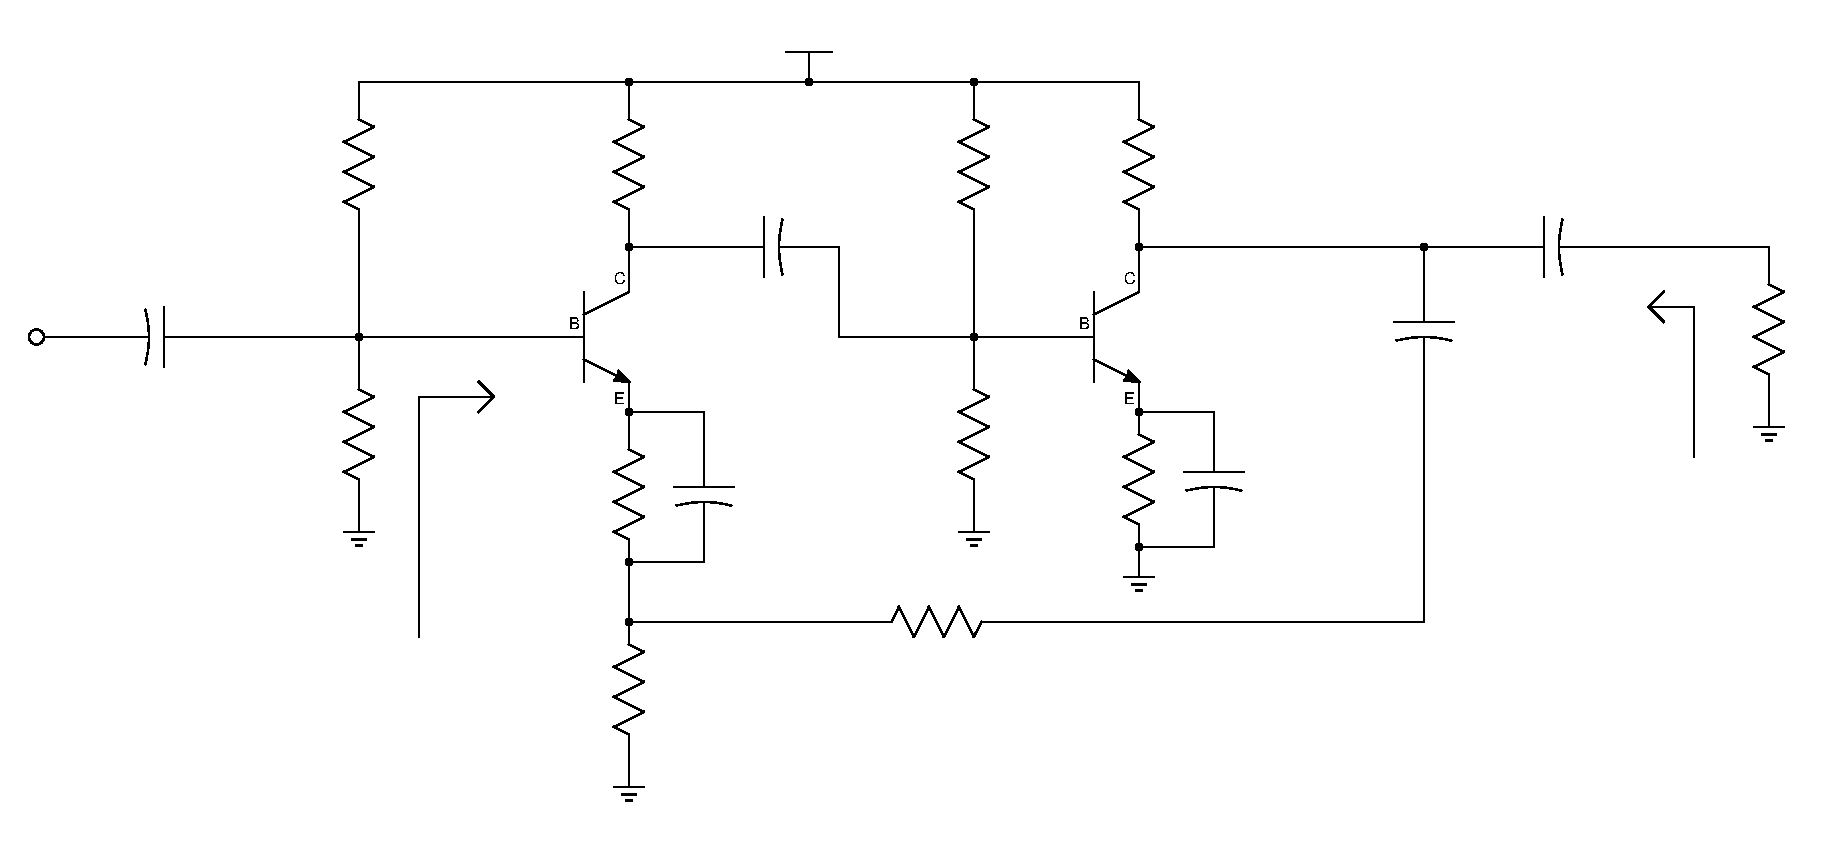
\includegraphics[scale=0.90]{voltageSeriesTwoStageAmplifier}
\caption{دو مرحلہ زنجیری واپسی برقی دباو ایمپلیفائر}
\label{شکل_واپسی_دو_درجہ_واپسی_برقی_دباو_ایمپلیفائر}
\end{figure}
اس ایمپلیفائر میں خارجی برقی دباو \عددیء{V_o} سے واپسی اشارہ \عددیء{V_f} حاصل کیا گیا ہے لہٰذا بنیادی ایمپلیفائر کے داخلی جانب کا دور حاصل کرتے وقت خارجی نقطے  کو قصر دور کیا جائے گا۔چونکہ \عددیء{V_o} کو  \عددیء{R_L} پر ناپا جاتا ہے لہٰذا خارجی نقطے  کو قصر دور کرنے سے مراد اس نقطے  کو برقی زمین کے ساتھ جوڑنا ہے۔شکل \حوالہ{شکل_واپسی_دو_درجہ_واپسی_برقی_دباو_ایمپلیفائر_داخلی_حصہ} الف میں ایسا دکھایا گیا ہے۔جیسا کہ شکل  ب میں دکھایا گیا ہے، اس عمل سے \عددیء{R_{f1}} اور \عددیء{R_{f2}} متوازی جڑ جاتے ہیں۔
\begin{figure}
\centering
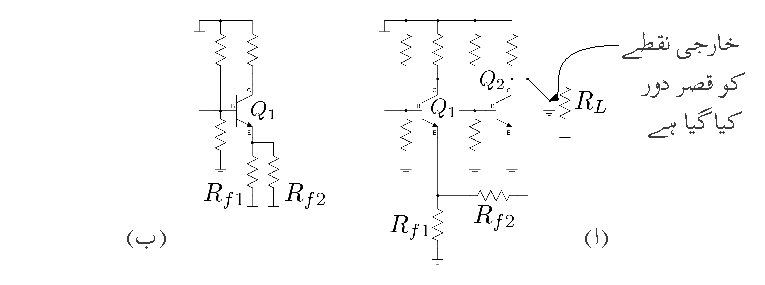
\includegraphics[scale=0.90]{voltageSeriesTwoStageAmplifierA}
\caption{دو مرحلہ زنجیری واپسی برقی دباو ایمپلیفائر کے داخلی حصے کا حصول}
\label{شکل_واپسی_دو_درجہ_واپسی_برقی_دباو_ایمپلیفائر_داخلی_حصہ}
\end{figure}
اس ایمپلیفائر میں \عددیء{V_f} اور \عددیء{V_s} سلسلہ وار جڑے ہیں لہٰذا بنیادی ایمپلیفائر کے خارجی جانب کا دور حاصل کرتے وقت داخلی دائرے کو کھلے دور کیا جائے گا۔اس دائرے کو \عددیء{Q_1} کے بیس یا اس کے ایمٹر پر کھلے دور کیا جا سکتا ہے۔شکل \حوالہ{شکل_واپسی_دو_درجہ_واپسی_برقی_دباو_ایمپلیفائر_خارجی_حصہ} الف  میں داخلی دائرے کو \عددیء{Q_1} کے ایمٹر پر کھلے دور کیا گیا ہے۔جیسا کہ شکل  ب میں دکھایا گیا ہے، اس عمل سے \عددیء{R_{f1}} اور \عددیء{R_{f2}} خارجی جانب سلسلہ وار جڑ جاتے ہیں۔
\begin{figure}
\centering
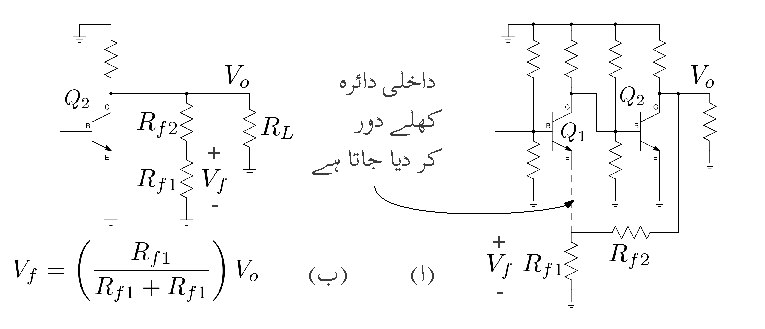
\includegraphics[scale=0.90]{voltageSeriesTwoStageAmplifierB}
\caption{دو مرحلہ زنجیری واپسی برقی دباو ایمپلیفائر کے خارجی حصے کا حصول}
\label{شکل_واپسی_دو_درجہ_واپسی_برقی_دباو_ایمپلیفائر_خارجی_حصہ}
\end{figure}
%
\begin{figure}
\centering
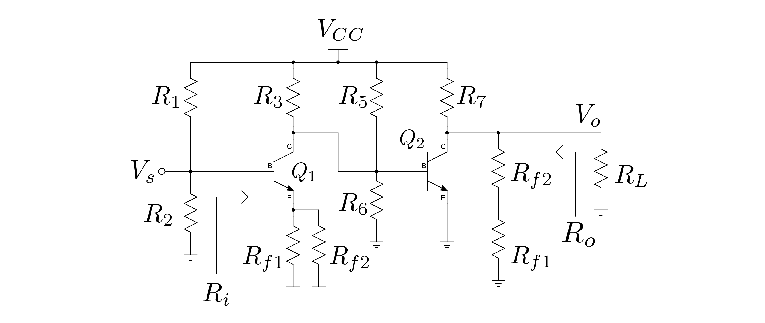
\includegraphics[scale=0.90]{voltageSeriesTwoStageAmplifierC}
\caption{دو مرحلہ زنجیری واپسی برقی دباو ایمپلیفائر کا بنیادی ایمپلیفائر}
\label{شکل_واپسی_دو_درجہ_واپسی_برقی_دباو_ایمپلیفائر_بنیادی}
\end{figure}
شکل \حوالہ{شکل_واپسی_دو_درجہ_واپسی_برقی_دباو_ایمپلیفائر_بنیادی} کو زنجیری ضرب سے با آسانی حل کرتے ہوئے \عددیء{A_v} حاصل کی جا سکتی ہے۔اسی  طرح اس بنیادی ایمپلیفائر کا \عددیء{R_i} اور \عددیء{R_o} بھی حاصل کیا جا سکتا ہے۔شکل سے واپس کار کا \عددیء{W} یوں حاصل ہوتا ہے۔
\begin{align}\label{مساوات_واپسی_زنجیری_ایمپلیفائر}
W=\frac{R_{f1}}{R_{f1}+R_{f2}}
\end{align}
ان تمام معلومات سے \عددیء{A_{vf}}، \عددیء{R_{if}'} اور \عددیء{R_{of}} حاصل کیا جا سکتا ہے۔

%=========================
\newpage
\حصہء{سوالات}

%========================
\ابتدا{سوال}\شناخت{سوال_واپسی_بگاڑ_بالمقابل_افزائش}
ایک سادہ ایمپلیفائر کی افزائش میں مختلف وجوہات کی بنا پر \عددیء{\SI{7}{\percent}} کے فرق پیدا ہوتا ہے۔اس ایمپلیفائر میں واپسی اشارہ شامل کیا جاتا ہے۔یوں حاصل واپسی ایمپلیفائر کی افزائش میں انہیں وجوہات کی بنا پر صرف \عددیء{\SI{1}{\percent}} کا فرق پیدا ہوتا ہے۔\عددیء{M} کی قیمت حاصل کریں۔اگر سادہ ایمپلیفائر کی افزائش \عددیء{\SI{245}{\volt \per \volt}} تھی تب واپسی ایمپلیفائر کے افزائش اور واپس کار کے مستقل \عددیء{W}  کی قیمت کیا ہو گی؟

جوابات:\عددیء{M=7}، \عددیء{A_f=\SI{35}{\volt \per \volt}}، \عددیء{W=\SI{0.02449}{\volt \per \volt}}
\انتہا{سوال}
%=================
\ابتدا{سوال}
اگر سوال \حوالہ{سوال_واپسی_بگاڑ_بالمقابل_افزائش} میں سادہ ایمپلیفائر کا بلند انقطاعی تعدد \عددیء{\SI{200}{\kilo \hertz}} ہو تب واپسی ایمپلیفائر کی بلند انقطاعی تعدد کیا ہو گی۔

جواب:\عددیء{\SI{1.4}{\mega \hertz}}
\انتہا{سوال}
%===============
\ابتدا{سوال}\شناخت{سوال_واپسی_برقی_دباو_ایمپلیفائر}
ایک واپسی برقی دباو ایمپلیفائر کے \عددیء{A_v'=\SI{2000}{\volt \per \volt}}، \عددیء{R_i=\SI{2}{\kilo \ohm}} اور \عددیء{R_o=\SI{500}{\ohm}} ہیں۔داخلی اشارے کی مزاحمت \عددیء{R_s=\SI{1}{\kilo \ohm}} جبکہ برقی بوجھ \عددیء{R_L=\SI{10}{\kilo \ohm}} ہیں۔اس ایمپلیفائر میں واپسی اشارہ شامل کیا جاتا ہے۔واپس کار کا مستقل \عددیء{W=\SI{0.01}{\volt \per \volt}} ہے۔واپسی ایمپلیفائر کی افزائش، داخلی مزاحمت اور خارجی مزاحمت حاصل کریں۔

جوابات:\عددیء{A_{vf}=\SI{95}{\volt \per \volt}}، \عددیء{R_{if}'=\SI{60}{\kilo \ohm}}، \عددیء{R_{of}=\SI{24}{\ohm}}  
\انتہا{سوال}
%=========================
\ابتدا{سوال}
ایک واپسی برقی رو ایمپلیفائر کے \عددیء{A_i=\SI{2000}{\ampere \per \ampere}}، \عددیء{R_i=\SI{500}{\ohm}} اور
 \عددیء{R_o=\SI{5}{\kilo \ohm}} ہیں۔داخلی اشارے کی مزاحمت \عددیء{R_s=\SI{5}{\kilo \ohm}} جبکہ برقی بوجھ \عددیء{R_L=\SI{1}{\kilo \ohm}} ہیں۔اس ایمپلیفائر میں واپسی اشارہ شامل کیا جاتا ہے۔واپس کار کا مستقل \عددیء{W=\SI{0.01}{\ampere \per \ampere}} ہے۔واپسی ایمپلیفائر کی افزائش، داخلی مزاحمت اور خارجی مزاحمت حاصل کریں۔

جوابات: \عددیء{A_{if}=\SI{94}{\ampere \per \ampere}}، \عددیء{R_{if}'=\SI{28}{\ohm}}، \عددیء{R_{of}=\SI{96}{\kilo \ohm}}
\انتہا{سوال}
%=============
\ابتدا{سوال}
ایک موصل نما ایمپلیفائر کے \عددیء{A_g=\SI{2000}{\ampere \per \volt}}، \عددیء{R_i=\SI{5}{\kilo \ohm}} اور
 \عددیء{R_o=\SI{500}{\ohm}} ہیں۔داخلی اشارے کی مزاحمت \عددیء{R_s=\SI{500}{\ohm}} جبکہ برقی بوجھ \عددیء{R_L=\SI{1}{\kilo \ohm}} ہیں۔اس ایمپلیفائر میں واپسی اشارہ شامل کیا جاتا ہے۔واپس کار کا مستقل \عددیء{W=\SI{0.01}{\volt \per \ampere}} ہے۔واپسی ایمپلیفائر کی افزائش، داخلی مزاحمت اور خارجی مزاحمت حاصل کریں۔

جوابات:\عددیء{A_{gf}=\SI{86}{\ampere \per \volt}}، \عددیء{R_{if}'=\SI{39}{\kilo \ohm}}، \عددیء{R_{of}=\SI{9.59}{\kilo \ohm}}
\انتہا{سوال}

%==============
\ابتدا{سوال}\شناخت{سوال_واپسی_مزاحمت_نما_ایمپلیفائر}
ایک مزاحمت نما ایمپلیفائر کے \عددیء{A_r'=\SI{2000}{\volt \per \ampere}}، \عددیء{R_i=\SI{500}{\ohm}} اور
 \عددیء{R_o=\SI{5}{\kilo \ohm}} ہیں۔داخلی اشارے کی مزاحمت \عددیء{R_s=\SI{5}{\kilo \ohm}} جبکہ برقی بوجھ \عددیء{R_L=\SI{10}{\kilo \ohm}} ہیں۔اس ایمپلیفائر میں واپسی اشارہ شامل کیا جاتا ہے۔واپس کار کا مستقل \عددیء{W=\SI{0.01}{\ampere \per \volt}} ہے۔واپسی ایمپلیفائر کی افزائش، داخلی مزاحمت اور خارجی مزاحمت حاصل کریں۔

جوابات:\عددیء{A_{rf}=\SI{93}{\volt \per \ampere}}، \عددیء{R_{if}'=\SI{32}{\ohm}}، \عددیء{R_{of}=\SI{238}{\ohm}}
\انتہا{سوال}
%===============
\ابتدا{سوال}\شناخت{سوال_واپسی_برقی_دباو_ایمپلیفائر_استعمال_کرتے_ہوئے}
آپ کے پاس \عددیء{\SI{2000}{\volt \per \volt}} کا برقی دباو ایمپلیفائر موجود ہے جس کا داخلی مزاحمت \عددیء{\SI{5}{\kilo \ohm}} اور خارجی مزاحمت \عددیء{\SI{500}{\ohm}} ہیں۔اس کو استعمال کرتے ہوئے واپسی برقی دباو کا ایمپلیفائر تخلیق دیں جس کی افزائش \عددیء{\SI{12.5}{\volt \per \volt}} ہو۔داخلی اشارے کی مزاحمت \عددیء{\SI{1}{\kilo \ohm}} اور برقی بوجھ \عددیء{\SI{1.5}{\kilo \ohm}} متوقع ہیں۔\عددیء{R_{if}'} اور \عددیء{R_{of}} بھی حاصل کریں۔

جوابات:\عددیء{R_i'=\SI{6}{\kilo \ohm}}، \عددیء{A_{v'}=\SI{1667}{\volt \per \volt}}، \عددیء{A_V=\SI{1250}{\volt \per \volt}} ہیں لہٰذا \عددیء{A_{vf}=\SI{12.5}{\volt \per \volt}} کی خاطر \عددیء{W=\SI{0.08}{\volt \per \volt}} درکار ہے۔\عددیء{R_{if}'=\SI{606}{\kilo \ohm}} اور \عددیء{R_{of}=\SI{4.95}{\ohm}} ہیں۔
\انتہا{سوال}
%======================
\ابتدا{سوال}
سوال \حوالہ{سوال_واپسی_برقی_دباو_ایمپلیفائر_استعمال_کرتے_ہوئے} میں تخلیق کئے گئے واپسی ایمپلیفائر پر اگر \عددیء{\SI{3}{\kilo \ohm}} کا بوجھ لادا جائے تو اس کی \عددیء{A_{vf}} کیا حاصل ہو گی۔

جواب:\عددیء{\SI{12.4}{\volt \per \volt}}۔بوجھ کی مزاحمت آدھی کرنے سے واپسی افزائش میں صرف \عددیء{\SI{0.8}{\percent}} کی تبدیلی آئی۔واپسی ایمپلیفائر یقیناً مستحکم ہے۔
\انتہا{سوال}
%================
\ابتدا{سوال}
سوال \حوالہ{سوال_واپسی_برقی_دباو_ایمپلیفائر_استعمال_کرتے_ہوئے} میں تخلیق کردہ واپسی ایمپلیفائر میں بنیادی ایمپلیفائر کو تبدیل کرتے ہوئے \عددیء{\SI{1500}{\volt \per \volt}} کا ایمپلیفائر  نسب کیا جاتا ہے۔ایسا کرنے سے \عددیء{A_{vf}} کی نئی قیمت کیا حاصل ہو گی؟

جواب:\عددیء{\SI{12.33}{\volt \per \volt}}۔بنیادی ایمپلیفائر کے افزائش میں \عددیء{\SI{25}{\percent}} تبدیلی سے واپسی ایمپلیفائر کے افزائش میں صرف \عددیء{\SI{1.36}{\percent}} کی تبدیلی پیدا ہوئی۔واپسی ایمپلیفائر کے مستحکم ہونے کی یہ ایک اچھی مثال ہے۔
\انتہا{سوال}
%================
\ابتدا{سوال}
ایک واپسی برقی دباو ایمپلیفائر میں \عددیء{V_s=\SI{150}{\milli \volt}}، \عددی{V_f=\SI{148}{\milli \volt}} اور \عددیء{V_o=\SI{12}{\volt}} پائے جاتے ہیں۔اس ایمپلیفائر کے \عددیء{W}، \عددیء{A_{vf}} اور \عددیء{A_V} حاصل کریں۔اگر بنیادی ایمپلیفائر کا \عددیء{R_i'=\SI{2}{\kilo \ohm}} اور \عددیء{R_o=\SI{1950}{\ohm}} ہوں تب \عددیء{R_{if}'} اور \عددیء{R_{of}} کیا ہوں گے۔

جوابات:\عددیء{W=\SI{0.01233}{\volt \per \volt}}، \عددیء{A_{vf}=\SI{80}{\volt \per \volt}}، \عددیء{A_V=\SI{6000}{\volt \per \volt}}، \عددیء{R_{if}'=\SI{150}{\kilo \ohm}} اور \عددیء{R_{of}=\SI{26}{\ohm}} ہیں۔
\انتہا{سوال}
%====================
\ابتدا{سوال}
بنیادی برقی رو ایمپلیفائر کی افزائش \عددیء{\SI{3000}{\ampere \per \ampere}} جبکہ اسی سے حاصل واپسی ایمپلیفائر کی افزائش \عددیء{\SI{15}{\ampere \per \ampere}} ہے۔\عددیء{R_i'=\SI{20}{\kilo \ohm}} اور \عددیء{R_o=\SI{15}{\kilo \ohm}} کی صورت میں \عددیء{R_{if}'} اور \عددیء{R_{of}} حاصل کریں۔

جوابات:\عددیء{R_{if}'=\SI{100}{\ohm}} اور \عددیء{R_{of}=\SI{3}{\mega \ohm}}
\انتہا{سوال}
%=======================
\ابتدا{سوال}\شناخت{سوال_واپسی_ٹرانزسٹر_برقی_دباو_الف}
شکل \حوالہ{شکل_واپسی_بنیادی_ایمپلیفائر_کا_حصول} الف میں \عددیء{\beta=100}، \عددیء{R_L=\SI{1}{\kilo \ohm}}، \عددیء{R_s=\SI{2}{\kilo \ohm}} اور \عددیء{I_{CQ}=\SI{1}{\milli \ampere}} ہیں۔\عددیء{A_{vf}}، \عددیء{R_{if}'} اور \عددیء{R_{of}} حاصل کریں۔

جوابات:\عددیء{r_{be}=\SI{2.5}{\kilo \ohm}}، \عددیء{A_V=\SI{22.22}{\volt \per \volt}}، \عددیء{A_{vf}=\SI{0.957}{\volt \per \volt}}، \عددیء{R_{if}'=\SI{103.5}{\kilo \ohm}} اور \عددیء{R_{of}=\SI{35}{\ohm}}
\انتہا{سوال}
%========================
\ابتدا{سوال}
سوال \حوالہ{سوال_واپسی_ٹرانزسٹر_برقی_دباو_الف} میں \عددیء{\beta} کی قیمت \عددیء{200} جبکہ \عددیء{I_{CQ}=\SI{1}{\milli \ampere}} ہی رکھتے ہوئے اسے دوبارہ حل کریں۔\عددیء{A_{vf}} میں کتنے فی صد تبدیلی رو نما ہوئی۔

جوابات:\عددیء{A_{vf}=\SI{0.978}{\volt \per \volt}}، \عددیء{R_{if}'=\SI{204.5}{\kilo \ohm}}، \عددیء{R_{of}=\SI{22.5}{\ohm}} اور تبدیلی تقریباً  \عددیء{\SI{2}{\percent}} ہے۔
\انتہا{سوال}
%=====================
\ابتدا{سوال}
شکل \حوالہ{شکل_واپسی_دو_درجہ_واپسی_برقی_دباو_ایمپلیفائر} میں زنجیری ایمپلیفائر دکھایا گیا ہے جبکہ مساوات \حوالہ{مساوات_واپسی_زنجیری_ایمپلیفائر} میں اس کے واپس کار کا مستقل \عددیء{W} حاصل کیا گیا ہے۔\عددی{A_{vf}} حاصل کریں۔

جواب: \عددیء{A_{vf} =1+\tfrac{R_{f2}}{R_{f1}}}

\انتہا{سوال}
